%        نمونه پایان‌نامه آماده شده با استفاده از کلاس TarbiatModares، نگارش 0.4
%        سجاد نوریان، دانشگاه تربیت مدرس،   
%-----------------------------------------------------------------------------------------------------
%        اگر قصد نوشتن پروژه کارشناسی را دارید، در خط زیر به جای msc، کلمه bsc و اگر قصد نوشتن رساله دکتری
%        را دارید، کلمه phd را قرار دهید. کلیه تنظیمات لازم، به طور خودکار، اعمال می‌شود.
% !TEX TS-program = xelatex
\documentclass[oneside,openany,12pt,msc]{TarbiatModares}
%       فایل commands.tex را حتماً به دقت مطالعه کنید؛ چون دستورات مربوط به فراخوانی بسته زی‌پرشین 
%       و دیگر بسته‌ها و ... در این فایل قرار دارد و بهتر است که با نحوه استفاده از آنها آشنا شوید.

% در این فایل، دستورها و تنظیمات مورد نیاز، آورده شده است.
%--------------------------------------------------------------Tarbiat Modares-----------------------------------------------------
\usepackage{algpseudocode}

\usepackage{multirow}
\usepackage{rotating}
\usepackage{lscape}

% در ورژن جدید زی‌پرشین برای تایپ متن‌های ریاضی، این سه بسته، حتماً باید فراخوانی شود
\usepackage{amsthm,amssymb,amsmath}
% بسته‌ای برای تنطیم حاشیه‌های بالا، پایین، چپ و راست صفحه
\usepackage[top=40mm, bottom=30mm, left=25mm, right=35mm]{geometry}
\setlength{\textwidth}{15cm}
\setlength{\oddsidemargin}{2mm}
\renewcommand{\baselinestretch}{1.5}     % ꉑ¬‰Ü‰‚ ¡‰Î‰Ï‰
% بسته‌‌ای برای ظاهر شدن شکل‌ها و تصاویر متن
\usepackage{graphicx}
% بسته‌ای برای رسم کادر
%\usepackage{framed} 
% بسته‌‌ای برای چاپ شدن خودکار تعداد صفحات در صفحه «معرفی پایان‌نامه»
\usepackage{lastpage}
% بسته‌ و دستوراتی برای ایجاد لینک‌های رنگی با امکان جهش
\usepackage[linktocpage=true,colorlinks,pagebackref=true,linkcolor=blue,citecolor=magenta]{hyperref}
%\usepackage[pagebackref=false,colorlinks,linkcolor=blue,citecolor=magenta]{hyperref}
% چنانچه قصد پرینت گرفتن نوشته خود را دارید، خط بالا را غیرفعال و  از دستور زیر استفاده کنید چون در صورت استفاده از دستور زیر‌‌، 
% لینک‌ها به رنگ سیاه ظاهر خواهند شد که برای پرینت گرفتن، مناسب‌تر است
%\usepackage[pagebackref=false]{hyperref}
% بسته‌ لازم برای تنظیم سربرگ‌ها
\usepackage{fancyhdr}
% بسته‌ای برای ظاهر شدن «مراجع» و «نمایه» در فهرست مطالب
\usepackage[nottoc]{tocbibind}
% دستورات مربوط به ایجاد نمایه
\usepackage{makeidx}
\makeindex
%%%%%%%%%%%%%%%%%%%%%%%%%%
% فراخوانی بسته زی‌پرشین و تعریف قلم فارسی و انگلیسی
\usepackage{xepersian}
\settextfont[Scale=1.1]{XB Niloofar.ttf}

%%%%%%%%%%%%%%%%%%%%%%%%%%
% چنانچه می‌خواهید اعداد در فرمول‌ها، انگلیسی باشد، خط زیر را غیرفعال کنید
%\setdigitfont[Scale=0.9]{Persian Modern}
%\setdigitfont.ttf[Scale=1.1]{XB Zar}
%\setdigitfont[Scale.ttf=1.1]{B Nazanin Outline}
%%%%%%%%%%%%%%%%%%%%%%%.ttf%%%
% تعریف قلم‌های فارسی و انگلیسی اضافی بر.ttfای استفاده در بعضی از قسمت‌های متن
\defpersianfont\nastaliq[Scale=2.02]{IranNastaliq.ttf}
\defpersianfont\bnazaninout[Scale=2]{B Nazanin Outline.ttf} 
%\defpersianfont\chapternumber[Scale=2.5]{XB Kayhan Pook.ttf}
%\renewcommand{\chapternumber}[1][Scale=2.5]{\fontspec{XB Kayhan Pook.ttf}}
\defpersianfont\dav[Scale=2]{XB Kayhan Pook.ttf}
\defpersianfont\titr[Scale=1.02]{XB Titre.ttf}
\defpersianfont\chapternumber[Scale=3]{XB Niloofar.ttf}
%\renewcommand{\chapternumber}[1][Scale=3]{\fontspec{XB Niloofar.ttf}}

%%%%%%%%%%%%%%%%%%%%%%%%%%
% دستوری برای حذف کلمه «چکیده»
%\renewcommand{\abstractname}{}
% دستوری برای حذف کلمه «abstract»
\renewcommand{\latinabstract}{}
% دستوری برای تغییر نام کلمه «اثبات» به «برهان»
\renewcommand\proofname{\textbf{برهان}}
% دستوری برای تغییر نام کلمه «کتاب‌نامه» به «مراجع»
\renewcommand{\bibname}{کتاب‌نامه}
\def\contentsname{فهرست مندرجات}
\def\listfigurename{لیست اشکال}
% دستوری برای تعریف واژه‌نامه انگلیسی به فارسی
\newcommand\persiangloss[2]{#1\dotfill\lr{#2}\\}
% دستوری برای تعریف واژه‌نامه فارسی به انگلیسی 
\newcommand\englishgloss[2]{#2\dotfill\lr{#1}\\}
% تعریف دستور جدید «\پ» برای خلاصه‌نویسی جهت نوشتن عبارت «پروژه/پایان‌نامه/رساله»
\newcommand{\پ}{پروژه/پایان‌نامه/رساله }
%%%%%%%%%%%%%%%%%%%%%%%%%%
% تعریف و نحوه ظاهر شدن عنوان قضیه‌ها، تعریف‌ها، مثال‌ها و ...
\theoremstyle{definition}
\newtheorem{definition}{تعریف}[section]
\theoremstyle{theorem}
\newtheorem{theorem}[definition]{قضیه}
\newtheorem{lemma}[definition]{لم}
\newtheorem{proposition}[definition]{گزاره}
\newtheorem{corollary}[definition]{نتیجه}
\newtheorem{remark}[definition]{ملاحظه}
\theoremstyle{definition}
\newtheorem{example}[definition]{مثال}
\newcommand{\x}{\mbox{\boldmath$x$\unboldmath}}
\newcommand{\dd}{\mbox{\boldmath$d$\unboldmath}}
\newcommand{\Uu}{\mbox{\boldmath$U$\unboldmath}}
 \newcommand{\balpha}{\mbox{\boldmath$\alpha$\unboldmath}}
 \newcommand{\bbeta}{\mbox{\boldmath$\beta$\unboldmath}}
  \newcommand{\btheta}{\mbox{\boldmath$\theta$\unboldmath}}
 \newcommand{\bphi}{\mbox{\boldmath$\phi$\unboldmath}}
  \newcommand{\bpsi}{\mbox{\boldmath$\psi$\unboldmath}}
\newcommand{\bmu}{\mbox{\boldmath$\mu$\unboldmath}}
 \newcommand{\X}{\mbox{\boldmath$X$\unboldmath}}
\newcommand{\Y}{\mbox{\boldmath$Y$\unboldmath}}
\newcommand{\z}{\mbox{\boldmath$z$\unboldmath}}
 \newcommand{\W}{\mbox{\boldmath$W$\unboldmath}}
 \newcommand{\q}{\mbox{\boldmath$q$\unboldmath}}
 \newcommand{\bb}{\mbox{\boldmath$b$\unboldmath}}
 \newcommand{\I}{\mbox{\boldmath$I$\unboldmath}}
\newcommand{\w}{\mbox{\boldmath$w$\unboldmath}}
\newcommand{\tb}{\mbox{\boldmath$\theta$\unboldmath}}
\newcommand{\bSigma}{\mbox{\boldmath$\Sigma$\unboldmath}}
\newcommand{\bsigma}{\mbox{\boldmath$\sigma$\unboldmath}}
\newcommand{\logit}{{\rm{logit}}}
\newcommand{\rth}{{\rm{th}}}
\newcommand{\E}{{\rm{E}}}
\newcommand{\Var}{{\rm{Var}}}
\newcommand{\Pq}{{\rm{P}}}
\newcommand{\ICHS}{مطالعه سلامت کودکان اندونزیایی}
\newcommand{\OR}{{\rm{OR}}}
\newcommand{\Corr}{{\rm{Corr}}}
\newcommand{\Cov}{{\rm{Cov}}}
%
%%%%%%%%%%%%%%%%%%%%%%%%%%%%
% دستورهایی برای سفارشی کردن سربرگ صفحات
\csname@twosidefalse\endcsname
\pagestyle{fancy}
\fancyhf{} 
\fancyhead[RE]{\rightmark}
\fancyhead[LO]{\leftmark}
\fancyhead[LE,RO]{\thepage}
\renewcommand{\chaptermark}[1]{%
\markboth{\thechapter.\ #1}{}}
% دستورهایی برای سفارشی کردن سربرگ صفحات
%\csname@twosidetrue\endcsname
%\pagestyle{fancy}
%\fancyhf{} 
%\fancyhead[OL,EL]{\thepage}
%\fancyhead[OR]{\small\rightmark}
%\fancyhead[ER]{\small\leftmark}
%\renewcommand{\chaptermark}[1]{%
%\markboth{\thechapter.\ #1}{}}
%%%%%%%%%%%%%%%%%%%%%%%%%%%%%
% دستورهایی برای سفارشی کردن صفحات اول فصل‌ها
\makeatletter
\newcommand\mycustomraggedright{%
 \if@RTL\raggedleft%
 \else\raggedright%
 \fi}
\def\@part[#1]#2{%
\ifnum \c@secnumdepth >-2\relax
\refstepcounter{part}%
\addcontentsline{toc}{part}{\thepart\hspace{1em}#1}%
\else
\addcontentsline{toc}{part}{#1}%
\fi
\markboth{}{}%
{\centering
\interlinepenalty \@M
\ifnum \c@secnumdepth >-2\relax
 \Huge\bfseries \partname\nobreakspace\thepart
\par
\vskip 20\p@
\fi
\Huge\bfseries #2\par}%
\@endpart}

\def\@makechapterhead#1{%
\vspace*{50pt} 
%\vspace*{-30\p@}%
{\parindent \z@ \mycustomraggedright 
%{\parindent 0pt \mycustomraggedright 
{\centering{
\ifnum \c@secnumdepth >\m@ne
\if@mainmatter

%\huge\bfseries \@chapapp\space {\chapternumber\thechapter}
%\huge\bnazaninout \@chapapp\space {\chapternumber\thechapter}
{\large\bnazaninout \@chapapp{} \thechapter \par}
\par\nobreak
\vskip 20\p@
\fi
% \vskip 20pt 
\fi
\interlinepenalty\@M 
\Huge \bfseries #1\par\nobreak  \vskip 120\p@  }}}}
% \Huge \bf #1       \par \nobreak \vskip 40pt }}}}
\makeatother
%%%%%%%%%%%%%%%%%%%%%%%%%%%%
%دستورات مربوط به نحوه شماره‌دهی جدول ها و شکل‌ها
\makeatletter 
\renewcommand \theequation {\@arabic\c@equation.\@arabic\c@section.\@arabic\c@chapter}
\renewcommand \thefigure     {\@arabic\c@figure.\@arabic\c@section.\@arabic\c@chapter}
\renewcommand \thetable      {\@arabic\c@table.\@arabic\c@section.\@arabic\c@chapter}
% دستوری برای حذف خط در زیر سربرگ هر صفحه
\renewcommand{\headrulewidth}{0pt}
\makeatother
%%%%%%%%%%%%%%%%%%%%%%%%%%%%
\begin{document}
% در این فایل، عنوان پایان‌نامه، مشخصات خود، متن تقدیمی‌، ستایش، سپاس‌گزاری و چکیده پایان‌نامه را به فارسی، وارد کنید.
% توجه داشته باشید که جدول حاوی مشخصات پایان‌نامه/رساله و همچنین، مشخصات داخل آن، به طور خودکار، درج می‌شود.
%%%%%%%%%%%%%%%%%%%%%%%%%%%%%%%%%%%%
% دانشگاه خود را وارد کنید
\university{تربیت مدرس}
% دانشکده، آموزشکده و یا پژوهشکده  خود را وارد کنید
\faculty{علوم ریاضی}
% گروه آموزشی خود را وارد کارشناسی ارشد آمار (رشته)}
\degree {کارشناسی ارشد علوم کامپیوتر}

% گروه آموزشی خود را وارد کنید
\subject{علوم کامپیوتر }
% گرایش خود را وارد کنید
\field{داده کاوی}
% عنوان پایان‌نامه را وارد کنید
\title{روش های عمیق مبتنی برمبدل های بینایی در تحلیل داده های تصویری}
% نام استاد(ان) راهنما را وارد کنید
\firstsupervisor{آقای دکتر منصور رزقی}
%\secondsupervisor{استاد راهنمای دوم}
% نام استاد(دان) مشاور را وارد کنید. چنانچه استاد مشاور ندارید، دستور پایین را غیرفعال کنید.
%\firstadvisor{نام استاد(دان) مشاور}
%نام استاد مشاور را وارد کنید. چنانچه دو استاد مشاور دارید  دستور پایین را نیز فعال کنید.
%\secondadvisor{نام استاد(دان) مشاور}
% نام پژوهشگر را وارد کنید
\name{سید محمد}
% نام خانوادگی پژوهشگر را وارد کنید
\surname{بادزهره}
% تاریخ پایان‌نامه را وارد کنید
\thesisdate{تابستان ۱۴۰۴}
% کلمات کلیدی پایان‌نامه را وارد کنید
%\keywords{داده‌های بقا فضایی، مدل‌های شکنندگی فضایی}
% چکیده پایان‌نامه را وارد کنید
\newpage
%\fa-abstract{\noindent
%در 

%}
%\newpage
\thispagestyle{empty}
\vtitle
%\newpage
%\thispagestyle{empty}
%\clearpage
%~~~
%\newpage
%\thispagestyle{empty}
%\input{rights}
%\newpage
%\thispagestyle{empty}
%\clearpage
%~~~
%\newpage
%\thispagestyle{empty}
%\centerline{{\includegraphics[width=20 cm]{replyrecord}}}
%\newpage
%\thispagestyle{empty}
%\clearpage
%~~~
\newpage
 % پایان‌نامه خود را تقدیم کنید!
\begin{acknowledgementpage}

\vspace{4cm}

{\nastaliq
{\Large
 تقدیم به
\vspace{1.5cm}

\newdimen\xa
\xa=\textwidth
% \advance \xa by -14cm
% \hspace{\xa}
پدر بزرگوار و مادر مهربانم و برادر عزیزم 
\newline
آن ها که از خواسته هایشان گذشتند، سختی ها را به جان خریدند و خود را سپر بلای مشکلات و ناملایمات کردند تا من به جایگاهی که اکنون در آن ایستاده ام برسم .


% \vspace{1.5cm}

\newdimen\xa
\xa=\textwidth
\advance \xa by -12cm
\hspace{\xa}
%...
\vspace{1.5cm}

\newdimen\xa
\xa=\textwidth
\advance \xa by -10cm
\hspace{\xa}

\vspace{1.5cm}

\newdimen\xa
\xa=\textwidth
\advance \xa by -8cm
\hspace{\xa}
}}
\end{acknowledgementpage}
%\newpage
%\thispagestyle{empty}
%\clearpage
%~~~
%%%%%%%%%%%%%%%%%%%%%%%%%%%%%%%%%%%%
%\newpage
%\thispagestyle{empty}
% ستایش
%\baselineskip=.750cm
%\ \\ \\
% 
%{\nastaliq
%رسيدن، به دانش است و به كردار نیک...%
%}\\
%\vspace{.5cm}\\
%{\scriptsize\nastaliq
%{
% و 
% }}
% 
%\vspace{.5cm}
%{\nastaliq
%\newdimen\xb
%\xb=\textwidth
%\advance \xb by -8.5cm
%\hspace{\xb}
%پس منطق ناگزير آمد بر جوينده‌ی رستگاری.
%\RTLfootnote{مقدمه‌ی رساله‌ی منطق دانشنامه‌ی علائی، شیخ‌الرئیس ابن‌سینا}
%}
%\newpage
%\thispagestyle{empty}
%\clearpage
%~~~
%%%%%%%%%%%%%%%%%%%%%%%%%%%%%%%%%%%%
\newpage
\thispagestyle{empty}
%قدردانی
{\nastaliq
قدردانی \newline
 \newline
 
از استاد گرانقدر، جناب آقای دکتر رزقی که با راهنمایی‌های دلسوزانه و ارزشمند خود، همواره در مسیر تحقیق این پایان‌نامه یار و راهنمای من بودند، نهایت سپاس و قدردانی را دارم.
\newline

از خانواده عزیزم که با محبت بی‌پایان، صبوری و حمایت‌های بی‌دریغ‌شان، همواره پشتیبان من در طی این مسیر سخت و پرچالش بودند، صمیمانه سپاسگزارم.

}
{\scriptsize\nastaliq
%سپاس و ستایش خدایی را که هستی نام ازو یافت، فلک جنبش، زمین آرام ازو یافت.
}


% با استفاده از دستور زیر، امضای شما، به طور خودکار، درج می‌شود
\signature 
%
\newpage
\thispagestyle{empty}
\baselineskip=1.0cm
\ \\ \\
\begin{large}
\begin{center}
چکیده
\end{center}
\end{large}
%}}
%\\[4cm]
ببعلعذدقفلهعقفدلخقفدللقفلقفاقا
%\newpage
%\thispagestyle{empty}
%\clearpage
%~~~
%\newpage
%{\small
%\abstractview
%}
%\newpage
%\thispagestyle{empty}
%\clearpage
%~~~
\newpage
\pagenumbering{harfi}
\pagenumbering{alph}
\tableofcontents
\listoftables
\listoffigures
\clearpage{\pagestyle{empty}\cleardoublepage}
\pagenumbering{arabic}
{
\baselineskip=1.0cm
\chapter*{پیش‌گفتار}
\phantomsection
\addcontentsline{toc}{chapter}{پیش‌گفتار}
\markboth{پیش‌گفتار}مقدثثمقدکنقصدبثقلدقفخدلقخفادخفادخ

\chapter{مفاهیم اولیه}
در این فصل به معرفی مقدمات و مفاهیم مورد نیاز در این پایان‌نامه می‌پردازیم. 
\section{مقدمه}
در این بخش به تاریخچه هوش مصنوعی، دستاورد های اولیه، چالش ها، دلایل رکود هوش مصنوعی و پایان عصر تاریک هوش مصنوعی صحبت میکنیم 

% update the abstract


\chapter{مفاهیم اولیه}

در این فصل به معرفی مقدمات و مفاهیم مورد نیاز در این پایان‌نامه می‌پردازیم.

\section{مقدمه}

در این بخش به تاریخچه هوش مصنوعی، دستاوردهای اولیه، چالش‌ها، دلایل رکود هوش مصنوعی و پایان عصر تاریک هوش مصنوعی صحبت می‌کنیم.

\subsection{آغاز هوش مصنوعی و هدف اصلی}

هوش مصنوعی به عنوان شاخه‌ای از علوم کامپیوتر، در دهه ۱۹۵۰ با هدف ساخت سیستم‌ها و ماشین‌هایی که توانایی تقلید از هوش انسانی را دارند، آغاز شد. نخستین بار، مکارتی در سال ۱۹۵۶ این اصطلاح را به کار گرفت \cite{mccarthy1956proposal} و هوش مصنوعی به عنوان علمی که در آن به مطالعه الگوریتم‌هایی برای تقلید رفتار انسانی می‌پردازد، شناخته شد. اهداف اولیه هوش مصنوعی شامل توانایی درک زبان، یادگیری، حل مسئله و تولید موجودات هوشمند بود. در این دوران پروژه‌های تحقیقاتی زیادی به امید دستیابی به هوش مصنوعی عمومی 
(\lr{AGI, Artificial General Intelligence})
شروع به کار کردند \cite{crevier1993ai,nilsson2010quest}.

\subsection{دورهٔ طلایی و پیشرفت‌های اولیه}

در دههٔ ۵۰ و ۶۰ میلادی، هوش مصنوعی به عنوان یکی از پرچمداران پژوهش‌های نوین شناخته می‌شد. الگوریتم‌های اولیه با تکیه بر روش‌های منطقی و ریاضیاتی برای حل مسئله و بازی‌های ساده توسعه یافتند؛ مانند انواع الگوریتم‌های جستجوی درختی که در این دوره به وجود آمدند و زمینه‌ساز اولین دستاوردهای هوش مصنوعی در بازی‌های تخته‌ای همچون شطرنج شدند \cite{newell1959report}. در این دوران، پیشرفت‌های بیشتری در پردازش زبان طبیعی (\lr{NLP}) و سیستم‌های خبره (\lr{Expert Systems}) نیز صورت گرفت که این امید را در دانشمندان و محققان تقویت کرد که دستیابی به هوش مصنوعی عمومی به‌زودی ممکن خواهد بود \cite{feigenbaum1983handbook}.

\subsection{انتظارات بیش از حد و ظهور عصر تاریک}

با وجود پیشرفت‌های هوش مصنوعی، محدودیت‌های تکنولوژی (مثل عدم وجود \lr{GPU}های پرقدرت در آن زمان) و همچنین کمبود داده‌های کافی برای آموزش مدل‌های پیچیده‌تر، باعث شد که بسیاری از پروژه‌های تحقیقاتی نتوانند به نتایج پیش‌بینی‌شده دست یابند. در نتیجه، هوش مصنوعی در دههٔ ۷۰ به مرحله‌ای از رکود وارد شد که به آن عصر تاریک هوش مصنوعی یا \lr{AI Winter} می‌گویند \cite{lighthill1973artificial,crevier1993ai}. در این دوران، بسیاری از پروژه‌ها تعطیل و سرمایه‌گذاری‌ها قطع شدند و دولت‌ها و سازمان‌های سرمایه‌گذار به دلیل عدم دستیابی به نتایج مطلوب از ادامهٔ سرمایه‌گذاری منصرف شدند.

\subsection{عوامل اصلی عصر تاریک هوش مصنوعی}

\begin{itemize}
	\item \textbf{محدودیت‌های سخت‌افزاری:}  
	در آن زمان، سیستم‌های اولیهٔ هوش مصنوعی به محاسبات سنگینی نیاز داشتند که با توان پردازشی محدود آن دوره همخوانی نداشت \cite{nilsson2010quest}.
	
	\item \textbf{کمبود داده‌ها:}  
	در آن زمان، دسترسی به داده‌های کافی برای آموزش مدل‌های پیچیده ممکن نبود و الگوریتم‌های موجود به داده‌های بیشتری نیاز داشتند تا بتوانند به‌درستی آموزش ببینند و عملکرد مطلوبی داشته باشند \cite{crevier1993ai}.
	
	\item \textbf{روش‌های محدود یادگیری:}  
	الگوریتم‌های اولیه به شدت به برنامه‌ریزی انسانی وابسته بودند و در بسیاری از موارد، مدل‌ها قادر به تعمیم به مسائل جدید نبودند و نمی‌توانستند تعمیم‌پذیری خیلی بالایی داشته باشند \cite{russell2016artificial}.
\end{itemize}

\subsection{پایان عصر تاریک و بازگشت هوش مصنوعی}

پس از چندین سال رکود و عدم سرمایه‌گذاری در حوزهٔ هوش مصنوعی، سرانجام در دههٔ ۱۹۸۰ و ۱۹۹۰ عصر تاریک هوش مصنوعی با تحولات تکنولوژی و از همه مهم‌تر ظهور سیستم‌های خبره (\lr{Expert Systems}) به پایان رسید \cite{feigenbaum1983handbook}. سیستم‌های خبره به عنوان یکی از اولین تلاش‌های موفق برای کاربردهای صنعتی در هوش مصنوعی به‌وجود آمدند. بر خلاف الگوریتم‌های اولیه، این سیستم‌ها از پایگاه بزرگ قواعد و قوانین (\lr{Rule-Based Systems}) استفاده می‌کردند. در سیستم‌های خبره، به جای تلاش برای شبیه‌سازی کلی هوش مصنوعی، بر حل مسائل تخصصی برای صنایع و سازمان‌ها تمرکز می‌شد. برای مثال، سیستم‌های خبره در پزشکی برای تشخیص بیماری‌ها و پیشنهاد درمان، در صنعت برای مدیریت و پیش‌بینی خرابی ماشین‌آلات، و در امور مالی برای تحلیل و ارزیابی ریسک کاربرد داشتند \cite{mccorduck2004machines}.

هرچند این سیستم‌ها نمی‌توانستند درک عمیق و هوشمندی عمومی را ایجاد کنند، اما برای رفع نیازهای پیچیده مناسب بودند. همزمان با موفقیت این سیستم‌ها، بهبودهای زیادی در سخت‌افزارها و کاهش هزینه‌های پردازش به وجود آمد. در دهه‌های ۱۹۸۰ و ۱۹۹۰، کامپیوترها به تدریج قوی‌تر و مقرون به صرفه‌تر شدند و امکان پردازش داده‌های بیشتر و اجرای الگوریتم‌های پیچیده‌تر فراهم شد. این افزایش توان محاسباتی، نیاز به پردازش داده‌های بزرگ و پیچیده را برآورده کرد و در نتیجه دسترسی به داده‌ها و انجام محاسبات سنگین برای توسعهٔ الگوریتم‌های جدید تسهیل شد. از سوی دیگر، پیشرفت‌های انجام‌شده در ذخیره‌سازی داده و رشد اینترنت باعث دسترسی گسترده‌تر به داده‌ها و منابع اطلاعاتی گردید \cite{nilsson2010quest}.

به این ترتیب، مجموعه‌ای از عوامل، شامل ظهور سیستم‌های خبره، افزایش قدرت پردازش و دسترسی به داده‌های بیشتر، منجر به بازگشت هوش مصنوعی شد. این دوره نه تنها پایان عصر تاریک هوش مصنوعی بود، بلکه راه را برای الگوریتم‌های یادگیری ماشین و توسعهٔ شبکه‌های عصبی هموار کرد \cite{russell2016artificial}.


\section{انواع مدل یادگیری ماشین و شبکه‌های عصبی}\label{sec:ml-types}
یادگیری ماشین و شبکه‌های عصبی در سال‌های اخیر مورد توجه بسیاری قرار گرفته‌اند و در حوزه‌های متنوعی از جمله پردازش تصویر، پردازش زبان طبیعی و داده‌کاوی استفاده می‌شوند
\cite{bishop2006pattern,mitchell1997machine,murphy2012machine}.

\subsection{یادگیری ماشین: مروری کلی}
یادگیری ماشین (\lr{Machine Learning}) شاخه‌ای از هوش مصنوعی است که به مدل‌های محاسباتی این امکان را می‌دهد الگوها را از داده‌ها به شکل خودکار یاد بگیرند و بتوانند تصمیم‌گیری کنند
\cite{goodfellow2016deep,mitchell1997machine}.
در واقع، هدف یادگیری ماشین این است که مدل‌ها بتوانند از داده‌ها الگوها و روابط پنهان را استخراج کنند و به نتایج و تصمیم‌های قابل اعتماد دست یابند.

\subsection{تقسیم‌بندی‌های اصلی در یادگیری ماشین}
به طور کلی، یادگیری ماشین به سه دستهٔ اصلی تقسیم می‌شود:
\begin{itemize}
	\item یادگیری با نظارت (\lr{Supervised Learning})
	\item یادگیری بدون نظارت (\lr{Unsupervised Learning})
	\item یادگیری تقویتی (\lr{Reinforcement Learning})
\end{itemize}
این طبقه‌بندی در بسیاری از کتاب‌ها و مراجع مهم یادگیری ماشین مطرح شده است
\cite{bishop2006pattern,murphy2012machine}.

\subsection{یادگیری نظارت‌شده (\lr{Supervised Learning})}
یادگیری نظارت‌شده یکی از رایج‌ترین روش‌ها در یادگیری ماشین شناخته می‌شود که در آن از مجموعه داده‌های برچسب‌گذاری‌شده برای آموزش مدل استفاده می‌کنیم
\cite{james2013introduction}. هدف این الگوریتم تشخیص الگوها در میان داده‌های ورودی است تا بتواند روی داده‌های جدید پیش‌بینی یا طبقه‌بندی انجام دهد. این نوع شامل دو دسته الگوریتمِ \lr{Regression} و \lr{Classification} می‌شود.

\subsubsection{طبقه‌بندی (\lr{Classification})}
طبقه‌بندی یکی از مهم‌ترین و اصلی‌ترین وظایف در یادگیری نظارت‌شده است که هدف آن تخصیص هر داده به یک لیبل مشخص است
\cite{bishop2006pattern}.
در این روش، مدل با داده‌های برچسب‌دار (Label) آموزش می‌بیند و یاد می‌گیرد که داده‌های جدید را بر اساس الگوها و ویژگی‌هایی که در داده‌های آموزشی دیده است، به دسته مناسب اختصاص دهد. از کاربردهای طبقه‌بندی می‌توان به تشخیص اسپم (\lr{Spam Detection})، تشخیص بیماری (مثلاً آیا یک فرد مبتلا به بیماری هست یا نه) و تشخیص چهره اشاره کرد
\cite{murphy2012machine}.

\subsubsection{رگرسیون (\lr{Regression})}
رگرسیون یکی از مهم‌ترین وظایف یادگیری ماشین است و هدف آن پیش‌بینی مقادیر پیوسته است
\cite{montgomery2021introduction}. بر خلاف طبقه‌بندی که خروجی آن یک دسته‌بندی مجزا است، در رگرسیون خروجی یک مقدار پیوسته خواهد بود و مدل می‌آموزد روابط بین متغیرهای مستقل و متغیر هدف را شناسایی کند. از کاربردهای رگرسیون می‌توان به پیش‌بینی قیمت مسکن یا پیش‌بینی آب‌وهوا اشاره کرد.

\subsection{یادگیری تقویتی (\lr{Reinforcement Learning})}
یادگیری تقویتی، نوعی یادگیری بر پایهٔ پاداش و تنبیه است که در آن مدل با محیط تعامل می‌کند و بر اساس پاداش یا تنبیه یاد می‌گیرد
\cite{sutton2018reinforcement}.
برخلاف یادگیری نظارت‌شده و بدون نظارت، یادگیری تقویتی به مدل این امکان را می‌دهد تا از طریق آزمون و خطا بهترین راهکارها را برای انجام یک عمل یاد بگیرد. در این روش، مدل به جای برچسب، از یک تابع پاداش استفاده می‌کند که مشخص می‌کند چه اقداماتی باعث نتیجهٔ بهینه می‌شود. از کاربردهای یادگیری تقویتی می‌توان به بازی‌ها (\lr{Games})، کنترل رباتیک (\lr{Robotic Control}) و سیستم‌های توصیه‌گر (\lr{Recommender Systems}) اشاره کرد.


\subsection{معرفی چند مدل از الگوریتم یادگیری کلاسیک}

\subsubsection{نزدیک‌ترین همسایه (\lr{k-Nearest Neighbors, kNN})}
الگوریتم \lr{kNN} یکی از روش‌های ساده و درعین‌حال کارآمد در یادگیری نظارت‌شده است که هم در دسته‌بندی و هم در رگرسیون کاربرد دارد
\cite{cover1967nearest,duda1973pattern,mitchell1997machine}.
این الگوریتم برای پیش‌بینی دسته‌بندی یک نمونهٔ جدید، به $k$ نزدیک‌ترین داده‌ها در فضای ویژگی نگاه می‌کند و بر اساس اکثریت نزدیکی همسایه‌ها، آن را به یک دسته اختصاص می‌دهد. 

\subsubsection{مزایا:}
\begin{itemize}
	\item \textbf{سادگی و قابل فهم بودن:}  
	این الگوریتم به سادگی با اندازه‌گیری فاصله بین نقاط داده کار می‌کند و بدون نیاز به آموزش مدل پیچیده قابل استفاده است
	\cite{cover1967nearest}.
	\item \textbf{عملکرد خوب در داده‌های با تعداد ویژگی کم:}  
	در مسائلی که تعداد ویژگی‌ها کم است، این الگوریتم اغلب به خوبی عمل می‌کند
	\cite{james2013introduction}.
\end{itemize}

\subsubsection{معایب:}
\begin{itemize}
	\item \textbf{حساسیت به داده‌های پرت:}  
	نقاط پرت می‌توانند به‌طور قابل توجهی بر نتایج تأثیر بگذارند
	\cite{duda1973pattern}.
	\item \textbf{کندی در داده‌های بزرگ:}  
	این الگوریتم نیاز به محاسبه فاصله برای هر نقطهٔ جدید دارد و در داده‌های بزرگ بار محاسباتی بالایی خواهد داشت
	\cite{mitchell1997machine}.
	\item \textbf{عدم کارایی در داده‌های با ابعاد بالا:}  
	در داده‌هایی با تعداد ویژگی‌های زیاد، کارایی الگوریتم کاهش می‌یابد \cite{murphy2012machine}.
\end{itemize}



\subsection{ماشین بردار پشتیبان (\lr{Support Vector Machine, SVM})}
الگوریتم \lr{SVM} با یافتن یک ابرصفحهٔ بهینه، داده‌ها را به کلاس‌های مختلف تقسیم می‌کند
\cite{cortes1995support,vapnik1998statistical}.
این الگوریتم یک ابرصفحه به دست می‌آورد که هدف آن حداکثر کردن فاصله میان داده‌های دو کلاس است و به این ترتیب می‌تواند طبقه‌بندی دقیقی داشته باشد.

\subsubsection{مزایا:}
\begin{itemize}
	\item \textbf{توانایی مقابله با داده‌های پیچیده و ابعاد بالا:}
	\lr{SVM} می‌تواند به خوبی با داده‌های چندبعدی و پیچیده کار کند
	\cite{vapnik1998statistical}.
	\item \textbf{مقاومت در برابر بیش‌برازش (\lr{Overfitting}):}
	با استفاده از هسته‌ها (\lr{kernels})، داده‌های غیرخطی نیز به فضای بالاتر برده می‌شوند و جداسازی بهتری انجام می‌شود
	\cite{cortes1995support}.
\end{itemize}

\subsubsection{معایب:}
\begin{itemize}
	\item \textbf{پیچیدگی محاسباتی:}
	آموزش \lr{SVM} به دلیل نیاز به حل مسائل بهینه‌سازی، در حجم‌های بالای داده محاسباتی زمان‌بر است
	\cite{murphy2012machine}.
	\item \textbf{کارایی پایین در داده‌های پرت:}
	در صورتی که داده‌ها شامل نقاط پرت زیادی باشند، دقت مدل کاهش می‌یابد
	\cite{bishop2006pattern}.
\end{itemize}


\subsection{بیز ساده (\lr{Naive Bayes})}
بیز ساده مبتنی بر قضیه بیز است و فرض می‌کند ویژگی‌ها به‌صورت شرطی مستقل از هم هستند
\cite{domingos1997optimal,mitchell1997machine}.
این مدل برای اولین بار در حوزهٔ پردازش متن به کار رفت و هنوز هم در بسیاری از کاربردها مانند طبقه‌بندی ایمیل و تحلیل احساسات مورد استفاده قرار می‌گیرد
\cite{mccallum1998comparison}. 
در \lr{Naive Bayes} بر اساس احتمالات محاسبه می‌شود که یک نمونهٔ جدید به کدام دسته تعلق دارد. این الگوریتم بر اساس قضیهٔ بیز، احتمال تعلق یک نمونه به هر دسته را به ازای هر ویژگی محاسبه کرده و در نهایت بالاترین احتمال را به‌عنوان جواب نهایی در نظر می‌گیرد
\cite{bishop2006pattern}.

\subsubsection{مزایا:}
\begin{itemize}
	\item \textbf{سرعت بالا}: به دلیل محاسبات ساده و فرض استقلال ویژگی‌ها، \lr{Naive Bayes} بسیار سریع و کم‌حجم است
	\cite{mccallum1998comparison}.
	\item \textbf{کارایی در داده‌های کوچک}: حتی با داده‌های کم، این الگوریتم عملکرد نسبتاً خوبی دارد
	\cite{murphy2012machine}.
\end{itemize}

\subsubsection{معایب:}
\begin{itemize}
	\item \textbf{فرض استقلال ویژگی‌ها}: فرض استقلال ویژگی‌ها ممکن است در بسیاری از مسائل واقعی صادق نباشد و این می‌تواند دقت مدل را کاهش دهد
	\cite{domingos1997optimal}.
	\item \textbf{حساسیت به داده‌های نادرست}: در صورت وجود داده‌های نادرست یا پرت، مدل ممکن است دقت کمتری داشته باشد
	\cite{bishop2006pattern}.
\end{itemize}


\subsection{شبکه‌های عصبی بازگشتی (\lr{RNN}) و شبکه‌های حافظه بلندمدت کوتاه‌مدت (\lr{LSTM})}
شبکه‌های عصبی بازگشتی (\lr{RNN}) و مدل‌هایی با حافظهٔ بلندمدت-کوتاه‌مدت (\lr{LSTM})
با هدف پردازش داده‌های ترتیبی و وابسته به زمان توسعه یافتند
\cite{rumelhart1986learning,hochreiter1997long}.
این مدل‌ها به‌ویژه در تحلیل زبان طبیعی، پردازش صوت و پیش‌بینی سری‌های زمانی بسیار موفق عمل کرده‌اند؛ زیرا قادر به حفظ اطلاعات گذشته هستند و از این اطلاعات برای پیش‌بینی در لحظهٔ حال و آینده استفاده می‌کنند
\cite{gers1999learning}.

\subsection{\lr{RNN}}
مدل‌های اولیهٔ شبکه‌های عصبی، مانند شبکه‌های چندلایه (\lr{MLP})، قادر به پردازش داده‌های مستقل و ثابت بودند و نمی‌توانستند وابستگی‌های زمانی را یاد بگیرند
\cite{bishop2006pattern}.
در بسیاری از مباحث دنیای واقعی مانند تحلیل متن و صدا، داده‌ها به توالی خاصی وابسته هستند. به همین دلیل، شبکه‌های \lr{RNN} معرفی شدند تا بتوانند از اطلاعات پیشین در پردازش داده‌های بعدی استفاده کنند
\cite{rumelhart1986learning}.

\subsubsection{ساختار و عملکرد \lr{RNN}}
شبکه‌های \lr{RNN} دارای حلقهٔ بازگشتی هستند که به مدل این امکان را می‌دهد اطلاعات را در توالی نگه دارد و در هر گام زمانی، ورودی فعلی \( x_t \) و وضعیت قبلی \( h_{t-1} \) را به‌عنوان ورودی دریافت کند
\cite{goodfellow2016deep}:

\begin{equation}
	h_t = \sigma \big( W \cdot x_t + U \cdot h_{t-1} + b \big)
\end{equation}

در اینجا:
\begin{itemize}
	\item \( h_t \) وضعیت مخفی یا حالت در گام زمانی \( t \) است.
	\item \( W \) وزن‌هایی است که به ورودی \( x_t \) اعمال می‌شود.
	\item \( U \) وزن‌های اعمال‌شده به وضعیت قبلی \( h_{t-1} \) است.
	\item \( b \) بایاس مدل است.
	\item \( \sigma \) تابع فعال‌سازی، معمولاً تانژانت هیپربولیک یا سیگموید.
\end{itemize}

با استفاده از این فرایند، مدل این توانایی را دارد که اطلاعات گذشته را در خود ذخیره کرده و در پردازش‌های بعدی از آن‌ها بهره ببرد.

\subsection{مزایا و معایب \lr{RNN}}
در این قسمت به مزایا و معایب شبکه‌های \lr{RNN} می‌پردازیم.

\subsubsection{مزایا:}
\begin{itemize}
	\item \textbf{حفظ وابستگی زمانی:}  
	\lr{RNN} قادر به پردازش توالی‌های طولانی است و می‌تواند اطلاعات را در طول توالی به خاطر بسپارد
	\cite{elman1990finding}.
	
	\item \textbf{کاربردهای گسترده در داده‌های ترتیبی:}  
	این مدل در تحلیل زبان طبیعی، پیش‌بینی سری‌های زمانی و پردازش صوت بسیار موفق عمل می‌کند
	\cite{gers1999learning}.
\end{itemize}

\subsubsection{معایب:}
\begin{itemize}
	\item \textbf{مشکل ناپدید شدن و انفجار گرادیان (\lr{Vanishing and Exploding Gradient}):}  
	در فرایند آموزش با روش پس‌انتشار، اگر توالی داده‌ها طولانی باشد، گرادیان‌ها ممکن است بسیار کوچک یا بزرگ شوند که منجر به ناپایداری در آموزش و کاهش دقت می‌شود
	\cite{hochreiter1998vanishing}.
	
	\item \textbf{محدودیت در پردازش توالی‌های بسیار بلند:}  
	\lr{RNN} در حفظ اطلاعات طولانی‌مدت با مشکل مواجه است و برای پردازش وابستگی‌های طولانی، عملکرد ضعیفی دارد
	\cite{hochreiter1997long,goodfellow2016deep}.
\end{itemize}

\subsection{شبکه‌های حافظه بلندمدت-کوتاه‌مدت (\lr{LSTM})}

\subsubsection{علل پیدایش \lr{LSTM}}
شبکه‌های \lr{LSTM} به عنوان یک راه‌حل برای یکی از بزرگ‌ترین مشکلات شبکه‌های عصبی بازگشتی (\lr{RNN}) معرفی شدند
\cite{hochreiter1997long}.
یکی از برجسته‌ترین مشکلات موجود در \lr{RNN}ها، معضل ناپدید شدن گرادیان (\lr{Vanishing Gradient}) بود که مانع یادگیری وابستگی‌های بلندمدت می‌شد
\cite{hochreiter1998vanishing,goodfellow2016deep}.
برای درک عمیق‌تر این مسأله، ابتدا به توضیح مشکل ناپدید شدن گرادیان و سپس راهکار \lr{LSTM} می‌پردازیم.

\subsubsection{\lr{Gradient Vanishing}}
شبکه‌های \lr{RNN} برای پردازش داده‌های ترتیبی از حلقه‌های بازگشتی بهره می‌برند. در فرایند آموزش \lr{RNN}، از الگوریتم پس‌انتشار خطا از طریق زمان (\lr{Backpropagation Through Time, BPTT}) استفاده می‌شود که گرادیان‌ها را جهت به‌روزرسانی وزن‌ها محاسبه می‌کند
\cite{rumelhart1986learning}.
با این حال، \lr{RNN}ها در یادگیری وابستگی‌های بلندمدت معمولاً ناکام می‌مانند. علت اصلی این امر شامل موارد زیر است:

\begin{itemize}
	\item \textbf{ضریب‌های بازگشتی کوچک‌تر از ۱:}
	در فرایند محاسبهٔ گرادیان‌ها، اگر مقدار مشتقات یا ضرایب در هر مرحله کوچک‌تر از ۱ باشد، ضرب مکرر این ضرایب در طول توالی منجر به کوچک‌شدن گرادیان‌ها به سمت صفر می‌شود؛ پدیده‌ای که به ناپدید شدن گرادیان معروف است
	\cite{hochreiter1998vanishing}.
\end{itemize}

فرمول کلی گرادیان در زمان \( t \) به‌صورت زیر است:
\[
\frac{\partial L}{\partial W} = \prod_{k=1}^{t} \frac{\partial h_k}{\partial h_{k-1}} \cdot \frac{\partial h_t}{\partial L},
\]
در این فرمول، \( \frac{\partial h_k}{\partial h_{k-1}} \) ممکن است مقداری کوچک‌تر از ۱ باشد، و ضرب مکرر آن در طول توالی باعث کاهش شدید مقدار گرادیان می‌گردد.

\begin{itemize}
	\item \textbf{تأثیر مستقیم بر وزن‌ها:}
	زمانی که گرادیان‌ها به صفر نزدیک می‌شوند، وزن‌های مدل عملاً به‌روزرسانی نمی‌شوند و این امر مانع از یادگیری وابستگی‌های طولانی‌مدت در داده‌ها می‌شود
	\cite{goodfellow2016deep}.
\end{itemize}

\subsection{ظهور \lr{LSTM}}
در سال ۱۹۹۷، \lr{Sepp Hochreiter} و \lr{J{\"u}rgen Schmidhuber} شبکه‌های حافظهٔ بلندمدت-کوتاه‌مدت (\lr{LSTM}) را معرفی کردند
\cite{hochreiter1997long}.
انگیزهٔ اصلی توسعهٔ \lr{LSTM} حل مشکل ناپدید شدن گرادیان در شبکه‌های \lr{RNN} بود. این مشکل در مسائل یادگیری داده‌های ترتیبی طولانی مانع می‌شد \lr{RNN} وابستگی‌های بلندمدت را به‌درستی فراگیرد.

\subsubsection{راه‌حل \lr{LSTM} برای پایداری جریان گرادیان‌ها}
\lr{LSTM} با معرفی معماری جدید در شبکه‌های بازگشتی، جریان گرادیان‌ها را در طول توالی پایدار نگه می‌دارد. این کار از طریق اضافه کردن وضعیت سلولی (\lr{Cell State}) و دروازه‌ها (\lr{Gates}) به ساختار \lr{RNN} انجام می‌شود
\cite{gers1999learning}.
این اجزا به \lr{LSTM} امکان می‌دهند:

\begin{enumerate}
	\item اطلاعات غیرضروری را فراموش کند،
	\item اطلاعات مهم جدید را اضافه کند،
	\item اطلاعات مهم قبلی را حفظ کند.
\end{enumerate}

\section{اختار \lr{LSTM}: نوآوری در مقایسه با \lr{RNN}}
\lr{LSTM} شامل اجزای جدیدی است که به آن امکان مدیریت بهتر اطلاعات را می‌دهد:

\subsection{وضعیت سلولی (\lr{Cell State})}
مسیر اصلی ذخیرهٔ اطلاعات در \lr{LSTM} است که می‌تواند اطلاعات مهم را در طول توالی حفظ کند. برخلاف \lr{RNN} که عمدتاً بر خروجی‌های بازگشتی \( h_t \) متکی است، \lr{LSTM} یک مسیر جداگانه برای عبور اطلاعات از وضعیت سلولی دارد که به حفظ گرادیان‌ها کمک شایانی می‌کند
\cite{hochreiter1997long}.

\subsection{دروازه‌ها (\lr{Gates})}
دروازه‌ها نقش فیلترهای اطلاعاتی را دارند که جریان اطلاعات را در طول فرایند یادگیری کنترل می‌کنند:

\begin{itemize}
	\item \textbf{دروازهٔ فراموشی (\lr{Forget Gate}):}
	تعیین می‌کند چه اطلاعاتی از وضعیت سلولی باید حذف شود
	\cite{gers1999learning}:
	\[
	f_t = \sigma \big( W_f \cdot [h_{t-1}, x_t] + b_f \big),
	\]
	\[
	f_t:\text{ میزان فراموشی برای هر عنصر از وضعیت سلولی},
	\]
	\[
	\sigma:\text{ تابع سیگموید (خروجی بین ۰ و ۱)}.
	\]
	در صورت \( f_t = 0 \)، اطلاعات حذف می‌شود و در صورت \( f_t = 1 \)، حفظ می‌شود.
	
	\item \textbf{دروازهٔ ورودی (\lr{Input Gate}):}
	تعیین می‌کند چه اطلاعات جدیدی باید به وضعیت سلولی اضافه شود:
	\[
	i_t = \sigma \big( W_i \cdot [h_{t-1}, x_t] + b_i \big),
	\]
	\[
	\tilde{C}_t = \tanh \big( W_C \cdot [h_{t-1}, x_t] + b_C \big),
	\]
	که در آن \( i_t \) میزان اطلاعات جدید و \( \tilde{C}_t \) مقدار جدید قابل اضافه‌شدن به وضعیت سلولی را نشان می‌دهد.
	
	\item \textbf{دروازهٔ خروجی (\lr{Output Gate}):}
	تعیین می‌کند چه اطلاعاتی از وضعیت سلولی به خروجی منتقل شود:
	\[
	o_t = \sigma \big( W_o \cdot [h_{t-1}, x_t] + b_o \big),
	\]
	\[
	h_t = o_t \cdot \tanh(C_t).
	\]
\end{itemize}

\subsection{به‌روزرسانی وضعیت سلولی}
وضعیت سلولی \( C_t \) با استفاده از اطلاعات جدید و قدیمی به‌روزرسانی می‌شود:
\[
C_t = f_t \cdot C_{t-1} + i_t \cdot \tilde{C}_t.
\]
این ساختار باعث می‌شود اطلاعات قدیمی مهم حفظ و داده‌های غیرضروری حذف شوند.

\subsubsection{علت پایداری گرادیان در \lr{LSTM}}
\begin{itemize}
	\item \textbf{حذف ضرب‌های مکرر:}
	برخلاف \lr{RNN} که به ضرب‌های مکرر وزن‌ها و گرادیان‌ها وابسته است، \lr{LSTM} با مسیر جداگانهٔ وضعیت سلولی، از کاهش نمایی گرادیان جلوگیری می‌کند
	\cite{hochreiter1998vanishing}.
	
	\item \textbf{استفاده از توابع سیگموید و تانژانت هیپربولیک:}
	توابع سیگموید در دروازه‌ها و تانژانت هیپربولیک در وضعیت سلولی مقادیر را محدود می‌کنند و مانع از انفجار گرادیان می‌شوند
	\cite{gers1999learning,goodfellow2016deep}.
	
	\item \textbf{مدیریت اطلاعات توسط دروازه‌ها:}
	دروازه‌های فراموشی و ورودی به مدل اجازه می‌دهند تنها اطلاعات مهم حفظ شود و داده‌های غیرضروری حذف شوند؛ این موضوع از پیچیدگی محاسباتی غیرضروری جلوگیری می‌کند
	\cite{hochreiter1997long}.
\end{itemize}


%\subsection{مقایسه RNN  و LStm:}


\begin{table}[h!]
	\centering
	\begin{tabular}{|c|c|c|}
		\hline
		\textbf{ویژگی} & \textbf{RNN} & \textbf{LSTM} \\ \hline
		\textbf{مشکل ناپدید شدن گرادیان} & وجود دارد & برطرف شده \\ \hline
		\textbf{توانایی حفظ وابستگی‌های طولانی‌مدت} & محدود به وابستگی کوتاه‌مدت & بسیار خوب \\ \hline
		\textbf{ساختار دروازه‌ها} & ندارد & دارای دروازه‌های فراموشی، ورودی و خروجی \\ \hline
		\textbf{پایداری گرادیان} & ضعیف & پایدار \\ \hline
	\end{tabular}
	\caption{مقایسه ویژگی‌های RNN و LSTM}
\end{table}



\subsection{مشکلات کلی \lr{RNN} و \lr{LSTM} و ظهور ترنسفورمرها}
شبکه‌های بازگشتی \lr{RNN} و \lr{LSTM} توانستند بسیاری از مشکلات و محدودیت‌های مدل‌های اولیه را حل کنند؛
اما همچنان با چالش‌ها و محدودیت‌هایی مواجه بودند که در مسائل پیچیده‌تر، مانند ترجمهٔ زبان یا تحلیل داده‌های بلندمدت و حجیم، مشکلات جدی ایجاد می‌کردند
\cite{hochreiter1997long,goodfellow2016deep}.
این مشکلات در نهایت به پیدایش ترنسفورمرها (\lr{Transformers}) منجر شد
\cite{vaswani2017attention}.
در ادامه، مهم‌ترین محدودیت‌های \lr{RNN} و \lr{LSTM} مورد بررسی قرار می‌گیرند.

\subsubsection{مشکل وابستگی ترتیبی در \lr{RNN}ها و \lr{LSTM}ها}
\lr{RNN}ها و \lr{LSTM}ها داده‌ها را به‌صورت ترتیبی پردازش می‌کنند؛ به این معنی که برای پردازش داده‌های گام زمانی \( t \)، باید تمامی داده‌های قبلی (\( t-1 \)) پردازش شده باشند
\cite{rumelhart1986learning,hochreiter1997long}.
این ویژگی مشکلات زیر را ایجاد می‌کند:
\begin{itemize}
	\item \textbf{غیرقابل موازی‌سازی:}  
	به دلیل وابستگی ترتیبی، پردازش داده‌ها به‌صورت موازی ممکن نیست و همین امر باعث افزایش زمان محاسباتی می‌شود. در داده‌های بلند (مانند متن‌های طولانی یا سری‌های زمانی بزرگ)، این مشکل نمود بیشتری دارد.
	
	\item \textbf{کندی آموزش و استنتاج:}  
	پردازش خطی داده‌ها موجب می‌شود زمان آموزش و پیش‌بینی مدل‌ها به‌شدت افزایش یابد، به‌ویژه زمانی که با حجم زیادی از داده مواجه هستیم.
\end{itemize}

\subsubsection{محدودیت در یادگیری وابستگی‌های بسیار طولانی}
با وجود پیشرفت \lr{LSTM} در یادگیری وابستگی‌های بلندمدت نسبت به \lr{RNN}های معمولی، این مدل‌ها همچنان در یادگیری وابستگی‌های بسیار بلند، مانند ارتباط بین کلمات در جملات دور از هم یا درک ساختار کلی یک متن، محدودیت دارند
\cite{hochreiter1998vanishing}:
\begin{itemize}
	\item \textbf{مشکل در داده‌های بسیار طولانی:}  
	حتی در \lr{LSTM} نیز ظرفیت حفظ اطلاعات محدود است و با افزایش طول توالی، دقت مدل افت می‌کند.
	
	\item \textbf{تأثیر تدریجی داده‌های اولیه:}  
	داده‌های ابتدایی توالی ممکن است با گذشت زمان اهمیت خود را از دست بدهند، چراکه گرادیان‌ها به‌تدریج ضعیف‌تر می‌شوند.
\end{itemize}

\subsubsection{پیچیدگی محاسباتی و حافظه}
\lr{LSTM}ها به علت ساختار پیچیده‌ای که شامل چندین ماتریس ضرب (برای دروازه‌های فراموشی، ورودی و خروجی) و به‌روزرسانی وضعیت سلول است، به حافظه و محاسبات زیادی نیاز دارند
\cite{goodfellow2016deep}:
\begin{itemize}
	\item \textbf{نیاز به حافظه بیشتر:}  
	برای ذخیرهٔ وضعیت سلولی و گرادیان‌ها، \lr{LSTM}ها به حافظهٔ بیشتری نسبت به مدل‌های ساده‌تر احتیاج دارند.
	
	\item \textbf{هزینهٔ محاسباتی بالا:}  
	در داده‌های حجیم، انجام محاسبات سنگین می‌تواند اجرای مدل را بسیار کند سازد.
\end{itemize}

\subsubsection{مشکل پردازش وابستگی‌های غیرمتوالی}
\lr{RNN}ها و \lr{LSTM}ها به‌طور طبیعی برای یادگیری وابستگی‌های محلی و متوالی مناسب هستند. اما در مسائلی مانند ترجمهٔ زبان یا تحلیل متون، روابط غیرمحلی و غیرمتوالی نیز اهمیت دارند
\cite{bahdanau2014neural}.
به‌عنوان مثال، در جمله‌ای طولانی ممکن است کلمه‌ای در ابتدای جمله با کلمه‌ای در انتهای جمله ارتباط معنایی داشته باشد. \lr{RNN}ها و \lr{LSTM}ها برای یادگیری این‌گونه وابستگی‌ها محدودیت دارند.

\subsubsection{گرادیان‌های ناپایدار و مشکلات بهینه‌سازی}
با وجود بهبودهایی که \lr{LSTM} نسبت به \lr{RNN} در پایداری گرادیان ارائه داد، هنوز هم:
\begin{itemize}
	\item \textbf{مسائل گرادیان‌های ناپایدار:}  
	در توالی‌های بسیار بلند، گرادیان‌ها ممکن است همچنان دچار کاهش یا حتی در مواردی انفجار شوند.
	
	\item \textbf{مشکلات بهینه‌سازی:}  
	در مسائلی با ساختار پیچیده، یافتن مینیمم مناسب تابع هزینه برای \lr{RNN}ها و \lr{LSTM}ها دشوار است.
\end{itemize}

\subsubsection{نیاز به مدلی با ظرفیت بیشتر و سرعت بالاتر}
\begin{itemize}
	\item \textbf{مدل‌های بزرگ‌تر:}  
	برای مسائل پیچیده‌تر، به مدل‌هایی با تعداد پارامتر بالاتر نیاز است؛ اما \lr{RNN}ها و \lr{LSTM}ها به‌دلیل محدودیت در حافظه و پردازش، پاسخ‌گوی این نیاز نیستند.
	
	\item \textbf{کارایی در داده‌های چندوجهی (\lr{Multimodal}):}  
	برای داده‌هایی که ترکیبی از اطلاعات متنی، صوتی و تصویری هستند، \lr{RNN}ها و \lr{LSTM}ها توانایی لازم جهت پردازش موازی این اطلاعات را ندارند.
\end{itemize}

در مجموع، وابستگی ترتیبی در \lr{RNN} و \lr{LSTM} مانعی اساسی برای استفاده از این مدل‌ها در مسائل پیچیده و بزرگ بود که درنهایت به ظهور ترنسفورمرها منتهی شد
\cite{vaswani2017attention}.
ترنسفورمرها با طراحی مبتنی بر موازی‌سازی و مکانیزم توجه (\lr{Attention Mechanism})، این محدودیت را برطرف کرده و راه‌حلی کارآمدتر برای پردازش داده‌های ترتیبی ارائه دادند.




\chapter{پیشینه پژوهش}


با توجه به مشکلات مطرح شده شبکه های بازگشتی، معماری جدیدی به نام مبدل ها \footnote{\lr{Transformer}} مطرح شد 
ظهور مبدل‌ها یکی از تحولات اساسی در حوزه پردازش زبان طبیعی \footnote{\lr{NLP}} و یادگیری ماشین به شمار می‌رود.\cite{vaswani2017attention,bahdanau2014neural}. 
این مدل‌ها باعث تغییرات عمده‌ای در نحوه ساخت و آموزش مدل‌های زبانی و همچنین در بسیاری از کاربردهای دیگر یادگیری ماشین شده‌اند و توانستند بسیاری از مشکلات مدل‌های قبلی را حل کنند\cite{devlin2018bert,radford2018improving}.
\section{مشکلات ترجمه ماشینی و مبدل ها}

در ابتدا، ترجمه ماشینی \footnote{\lr{machine translation}} یک چالش اساسی در زمینهٔ پردازش زبان طبیعی بود. مدل‌های اولیه‌ای مانند مدل‌های مبتنی بر قواعد \footnote{\lr{Rule-based Models}} برای ترجمه استفاده می‌شدند که در آن‌ها، ترجمه‌ها به‌صورت دستی با استفاده از قواعد زبانی مشخص تنظیم می‌شدند \cite{nagao1984framework,hutchins1986machine}. این روش‌ها هرچند دقیق بودند، اما محدودیت‌های زیادی داشتند و نمی‌توانستند ویژگی‌های پیچیده‌تر زبان را مدل‌سازی کنند.



سپس مدل‌های آماری \footnote{\lr{Statistical Models}} معرفی شدند \cite{brown1993mathematics,koehn2010statistical}. این مدل‌ها از داده‌های ترجمه‌شده برای آموزش مدل‌های آماری استفاده می‌کردند که احتمال ترجمه صحیح را براساس شواهد آماری محاسبه می‌کردند. مدل‌هایی مانند مدل‌های ترجمه آماری مبتنی بر جمله \footnote{\lr{Phrase-based Statistical Models}} \cite{koehn2003statistical} از این نوع بودند که قادر به ترجمه جملات بهتر از مدل‌های مبتنی بر قواعد بودند، اما هنوز هم در ترجمه‌های پیچیده با مشکلاتی روبه‌رو بودند.



بعد از این مدل‌ها، مدل‌های بازگشتی \footnote{\lr{Recurrent Models}} به وجود آمدند که مشکلات آن‌ها در فصل گذشته بیان شد \cite{elman1990finding,sutskever2014sequence}. در نهایت، این مشکلات باعث به وجود آمدن ترانسفورمرها شد \cite{bahdanau2014neural}.




\section{ظهور ترانسفورمرها}
در سال ۲۰۱۷، مقاله‌ای توسط گوگل \footnote{\lr{google}} منتشر شد که مفهوم جدیدی به نام مبدل ها \footnote{\lr{Transformers}} را معرفی کرد \cite{vaswani2017attention}. این مقاله به موضوع ترجمه ماشینی پرداخت و نشان داد که با استفاده از مکانیزم توجه می‌توان بسیاری از مشکلات مدل‌های قبلی را حل کرد \cite{luong2015effective}.

مدل‌های ترانسفورمر برخلاف مدل‌های قبلی که از پردازش سریالی استفاده می‌کردند، از پردازش موازی بهره می‌برند. این ویژگی به ترانسفورمرها اجازه می‌دهد که به‌طور همزمان به تمام بخش‌های ورودی توجه کنند. این قابلیت باعث شد که مبدل ها در پردازش تصویر و متن بسیار سریع‌تر و دقیق‌تر از مدل‌های قبلی عمل کنند \cite{vaswani2017attention}.

\section{معماری مبدل ها}
در \textbf{تصویر \ref{fig:transformer_architecture}}، معماری مبدل نمایش داده شده است و بخش‌ها و اجزای مختلف آن مشخص شده است. معماری ترانسفورمر از دو بخش اصلی تشکیل شده است:
\begin{itemize}
\item \textbf{رمزگذار \footnote{\lr{Encoder}}:}
وظیفهٔ رمزگذار این است که دادهٔ ورودی را دریافت کند و ویژگی‌های آن را استخراج کند.
\item \textbf{رمزگشا \footnote{\lr{Decoder}}:}
وظیفهٔ رمزگشا این است که ویژگی‌های استخراج‌شده را به زبان مقصد تبدیل کند.
\end{itemize}

\begin{figure}[h]
	\centering
	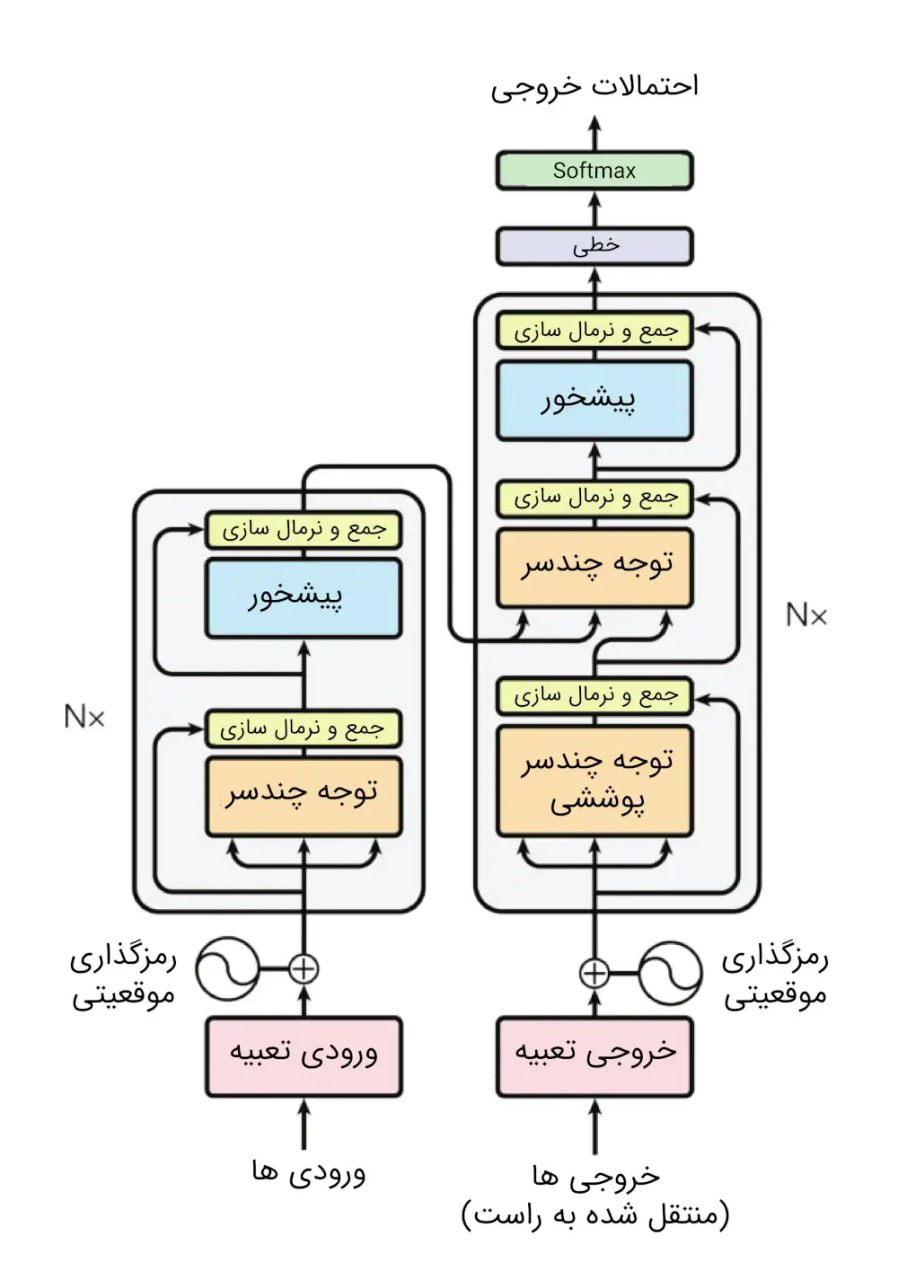
\includegraphics[width=0.65\textwidth]{transformer_images/persian images/b04.png}
	\caption{معماری ترانسفورمرها}
	\label{fig:transformer_architecture}
\end{figure}

\subsection{جاسازی}
در زبان طبیعی، کلمات به شکل رشته‌های متنی هستند مانند کتاب، ماشین و ... کامپیوترها نمی‌توانند به‌طور مستقیم این کلمات را به شکل رشته‌های متنی پردازش کنند. به همین دلیل، در یادگیری ماشین این کلمات را به شکل یک بردار نمایش می‌دهیم. این بردار بیانگر آن کلمه در مدل است تا ماشین بتواند آن کلمه را پردازش کند.

این بردارها ویژگی‌های کلمه را در فضای عددی نمایش می‌دهند. روش‌های مختلفی برای تبدیل متن به بردار وجود دارند. از جمله این روش‌ها می‌توان به روش‌های \lr{Word2Vec} \cite{mikolov2013distributed} و \lr{GloVe} \cite{pennington2014glove} اشاره کرد.

همان‌طور که در \autoref{fig:word_embedding} نشان داده شده است، هر کلمه که به صورت توکن است، ابتدا در دیکشنری تعریف‌شده پیدا می‌شود و پس از پیدا شدن در دیکشنری، با استفاده از روش‌های تعبیه کردن\footnote{\lr{Embedding}}، هر کلمه به برداری از اعداد تبدیل می‌شود. این جاسازی‌ها شباهت‌های معنایی بین کلمات را مدل‌سازی می‌کنند و کلماتی که از نظر معنایی شبیه به هم هستند، بردار آن‌ها نیز به یکدیگر نزدیک‌تر است. به این ترتیب، کلمات برای مدل‌ها و شبکه‌های عصبی قابل‌فهم می‌شوند \cite{mikolov2013distributed,pennington2014glove}.





 \begin{figure}[h]
 	\centering
 	\begin{minipage}[b]{0.7\textwidth}
 		\centering
 		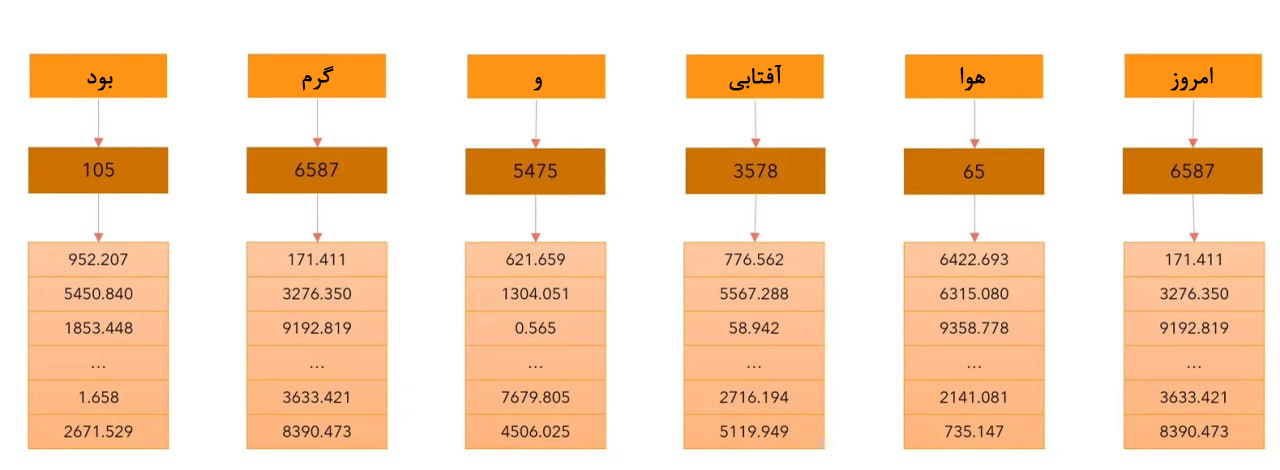
\includegraphics[width=\textwidth]{transformer_images/persian images/persian_images/b16.png}
 		\caption{جاسازی کلمه ای}
 		\label{fig:word_embedding}
 	\end{minipage}
 	\hfill
 \end{figure}
 
 
 

 
 
 
 



\subsection{جاسازی موقعیتی}

هر کلمه را به برداری از اعداد که برای مدل قابل فهم باشد، تبدیل کرده‌ایم. اما مدل‌های ترانسفورمر نمی‌توانند جایگاه هر کلمه را تشخیص دهند. در مدل‌های ترانسفورمر، برخلاف مدل‌های بازگشتی، به دلیل اینکه کلمات به‌صورت موازی وارد می‌شوند، نیاز داریم تا جایگاه هر کلمه را بدانیم. به‌طور مثال، در جملهٔ «من تو را دوست دارم» باید به‌طور دقیق بدانیم که «من» کلمهٔ اول جمله است، «تو» کلمهٔ دوم جمله است و ... .

حال باید به مدل توالی این کلمات را بفهمانیم. بنابراین، نیاز داریم به مدل یک سری اطلاعات اضافی بدهیم به‌طوری‌که مدل توالی کلمات را یاد بگیرد. روش‌های مختلفی برای اضافه‌کردن جاسازی موقعیتی \footnote{\lr{Positional Embedding}} به مدل وجود دارد. در ترانسفورمرها از روش جاسازی موقعیت سینوسی
 \footnote{\lr{Sinusoidal Positional Embedding}} استفاده می‌شود \cite{vaswani2017attention}.



این روش قابل یادگیری نیست و صرفاً از یک سری فرمول‌های ساده برای جاسازی موقعیتی استفاده می‌کند.  
برای موقعیت مشخص \footnote{\lr{pos}} در توالی و بُعد \( i \) در فضای برداری، تعبیه موقعیتی به‌صورت زیر تعریف می‌شود.  

و برای مقادیر زوج:  

\begin{equation}
	PE(pos, 2i) = \sin\left( \frac{pos}{10000^{\frac{2i}{d}}} \right)
	\label{eq:pe_even}
\end{equation}

و برای مقادیر فرد:  

\begin{equation}
	PE(pos, 2i+1) = \cos\left( \frac{pos}{10000^{\frac{2i}{d}}} \right)
	\label{eq:pe_odd}
\end{equation}
	



\begin{itemize}
	\item \( pos \): موقعیت کلمه در توالی است (مثلاً از \( 0 \) تا \( N-1 \) برای یک توالی \( N \)-تایی).
	\item \( i \): شاخص بعد در بردار موقعیتی (از \( 0 \) تا \( d-1 \) برای بعد فضای برداری \( d \)).
	\item \( d \): ابعاد فضای برداری مدل که نشان می‌دهد هر کلمه در چند بعد نمایش داده می‌شود.
	\item \( 10000 \): یک مقدار ثابت برای تنظیم مقیاس توابع تناوبی و ایجاد فرکانس‌های مختلف در ابعاد گوناگون.
\end{itemize}  

همان‌طور که در شکل \autoref{fig:word_embedding_positional_embedding} مشاهده می‌کنید، بعد از جاسازی کلمات، به آن جا سازی موقعیتی اضافه می‌شود. در این روش از توابع سینوس و کسینوس استفاده می‌شود. این توابع موقعیت‌ها را در فضای برداری به‌گونه‌ای نگاشت می‌کنند که مدل بتواند از ترتیب کلمات در توالی آگاه باشد \cite{vaswani2017attention}. این ویژگی به مدل کمک می‌کند تا توالی زمانی را درک کرده و الگوهای زمانی را شبیه‌سازی کند. از مزایای این روش می‌توان به عدم نیاز به آموزش و توزیع متوازن جایگاه کلمات اشاره کرد.

\begin{figure}[h]
	\centering
	\begin{minipage}[b]{0.7\textwidth}
		\centering
		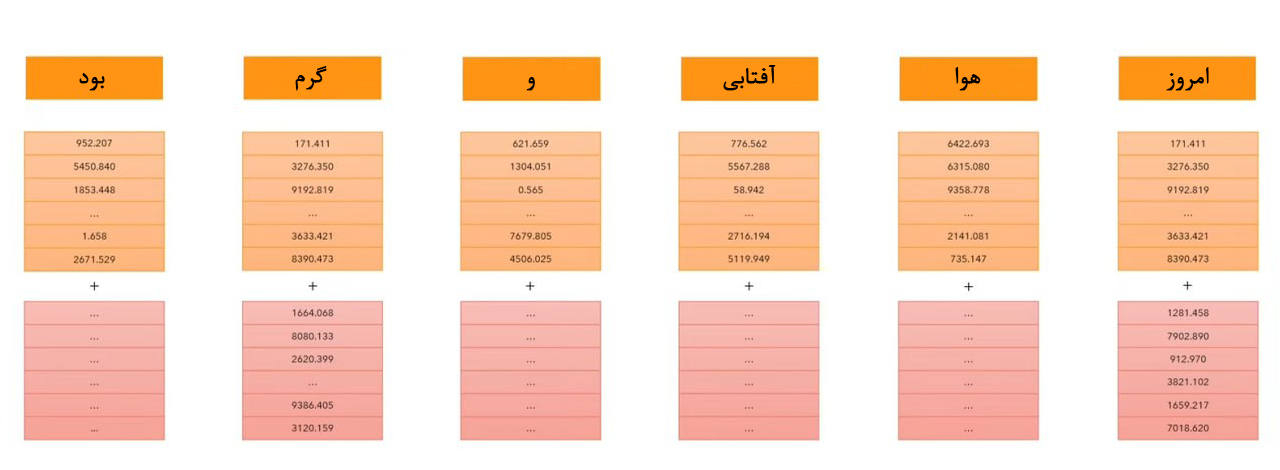
\includegraphics[width=\textwidth]{transformer_images/persian images/persian_images/b17.png}
		\caption{اضافه کردن جا سازی موقعیتی به جاسازی کلمه ای}
		\label{fig:word_embedding_positional_embedding}
	\end{minipage}
	\hfill
\end{figure}


\subsection{توجه}



در روش‌ شبکه های بازگشتی، توالی ورودی (مثلاً یک جمله) معمولاً به‌صورت گام‌به‌گام پردازش می‌شد \cite{elman1990finding,hochreiter1997long}. اما در ترانسفورمر می‌خواهیم مدلی داشته باشیم که به هر موقعیت (مثلاً یک کلمه) در توالی نگاه کند و به همهٔ موقعیت‌های دیگر نیز به‌صورت موازی دسترسی داشته باشد. به این مفهوم توجه\footnote{\lr{attention}} می‌گوییم.

به زبان ساده، وقتی توکن (کلمه) \( i \) به توکن‌های دیگر نگاه می‌کند، می‌خواهد بداند کدام توکن‌ها برای تفسیر معنای خودش مهم‌ترند.

به طور مثال در جمله‌ی «یک گربه روی زمین نشسته است» می‌خواهد بداند کلمه‌ی «گربه» به واژه‌ی «نشستن» بیشتر توجه کند یا به «زمین». در این‌جا فعل «نشستن» ارتباط نزدیک‌تری به «گربه» دارد و از نظر معنایی مرتبط‌تر است.


سه تا از اجزای اصلی یک توجه شامل موارد زیر است.

\[
Q = \text{Query (پرسش)}, \quad K = \text{Key (کلید)}, \quad V = \text{Value (مقدار / ارزش)}
\]





در  ضرب شباهت های توجه \footnote{\lr{Scaled Dot-Product Attention}}    \cite{vaswani2017attention}، ابتدا شباهت یا ارتباط بین پرسش \footnote{\lr{Query}} و کلید \footnote{\lr{Key}} را با محاسبهٔ ضرب داخلی \footnote{\lr{Dot Product}} به‌دست می‌آوریم، سپس آن را نرمال می‌کنیم (با تقسیم بر \( d_k \)) و از تابع سافت مکس \footnote{\lr{softmax}} استفاده می‌کنیم تا ضرایب توجه \footnote{\lr{Attention Weights}} را به‌دست آوریم. در نهایت با همین ضرایب، ترکیبی خطی از بردارهای مقدار \footnote{\lr{value}} را می‌گیریم.

فرمول به‌شکل زیر است:

\begin{equation}
	\text{Attention}(Q, K, V) = \text{softmax}\left( \frac{QK^T}{\sqrt{d_k}} \right) V
	\label{eq:attention}
\end{equation}

که در آن:

\[
Q \in \mathbb{R}^{n \times d_k} \quad \text{ماتریس پرسش برای }
\]
\[
K \in \mathbb{R}^{n \times d_k} \quad \text{ماتریس کلید برای }
\]
\[
V \in \mathbb{R}^{n \times d_v} \quad \text{ماتریس مقدار  }
\]



	 \( W^Q, W^K, W^V \in \mathbb{R}^{d_{model} \times d_k} \) ماتریس‌های وزنی قابل آموزش هستند که طی فرآیند یادگیری به‌روزرسانی می‌شوند.
	 
\begin{figure}[h]
	\centering
	\begin{minipage}[b]{0.7\textwidth}
		\centering
		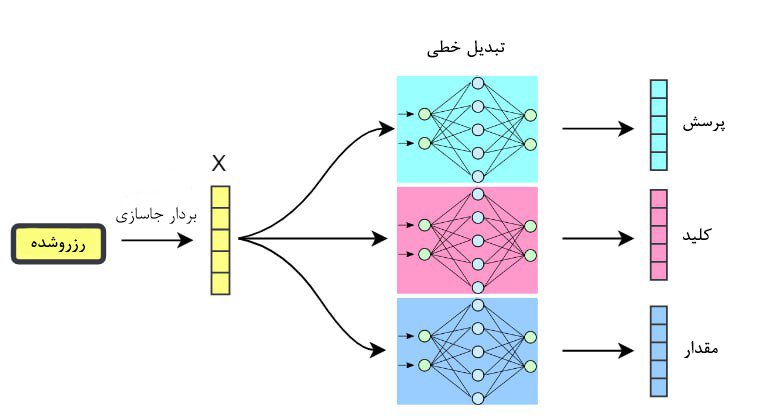
\includegraphics[width=\textwidth]{transformer_images/persian images/persian_images/b19.png}
		\caption{نحوه به دست آوردن پرسش، کلید و مقدار}
		\label{fig:qkv}
	\end{minipage}
	\hfill
\end{figure}


در واقع پرسش، کلید و مقدار با استفاه از mlp  تولید میشود.



تقسیم بر \( d_k \) باعث می‌شود مقدار ضرب داخلی در ابعاد بالا خیلی بزرگ نشود و شیب‌ها گرادیان پایدار بمانند.

\begin{equation}
	\alpha = \text{softmax}\left( \frac{QK^T}{\sqrt{d_k}} \right)
	\label{eq:alpha}
\end{equation}
\(\alpha\) یک ماتریس با ابعاد \( n \times n \) است که سطر \( i \)-ام آن ضرایب توجه برای توکن \( i \) را نشان می‌دهد.

تفسیر ضرایب توجه: هر سطر از \( \alpha \) نشان می‌دهد که توکن فعلی به چه توکن‌هایی در جمله، با چه شدتی توجه می‌کند.



\begin{figure}[h]
	\centering
	\begin{minipage}[b]{0.6\textwidth}
		\centering
		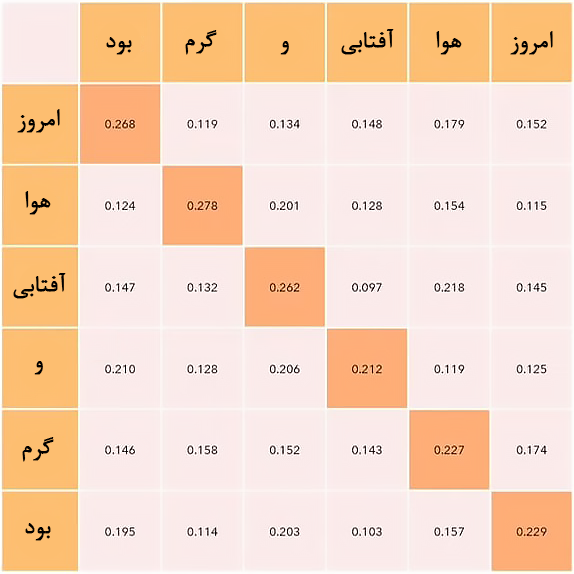
\includegraphics[width=\textwidth]{transformer_images/persian images/persian_images/b18.png}
		\caption{توجه}
		\label{fig:attention}
	\end{minipage}
	\hfill
	
\end{figure}



\subsection{توجه چند سر}



در ایده چند سری \footnote{\lr{multi head attention}}  
به‌جای آنکه فقط یک‌بار \( Q, K, V \) بسازیم و عملیات توجه را انجام دهیم، چندین مجموعهٔ متفاوت \( Q_i, K_i, V_i \) می‌سازیم (هر کدام یک «سر» \footnote{\lr{head}} نام دارد) و به‌صورت موازی محاسبات توجه را انجام می‌دهیم. سپس خروجی همهٔ این سرها را کنار هم قرار داده \footnote{\lr{concatenate}} و در نهایت با یک ماتریس وزن دیگر ضرب می‌کنیم تا به بعد اصلی بازگردیم.

فرمول مربوط به این ایده به‌شکل زیر است:


\begin{equation}
	\text{head}_i = \text{Attention}(Q_i, K_i, V_i)
	\label{eq:head_i}
\end{equation}


\begin{equation}
	\text{MultiHead}(Q, K, V) = [\text{head}_1 \oplus \cdots \oplus \text{head}_h] W_O
	\label{eq:multihead}
\end{equation}

که در آن \( \oplus \) نشان‌دهندهٔ عمل الحاق \footnote{\lr{concatenate}} است.

ماتریس وزن \( W_O \) به‌شکل زیر است:

\[
W_O \in \mathbb{R}^{(h \cdot d_v) \times d_{\text{model}}}
\]

که \( W_O \) ماتریسی است که خروجی الحاق‌شده را به بعد \( d_{\text{model}} \) برمی‌گرداند.





\begin{figure}[h]
	\centering
	\begin{minipage}[b]{0.9\textwidth}
		\centering
		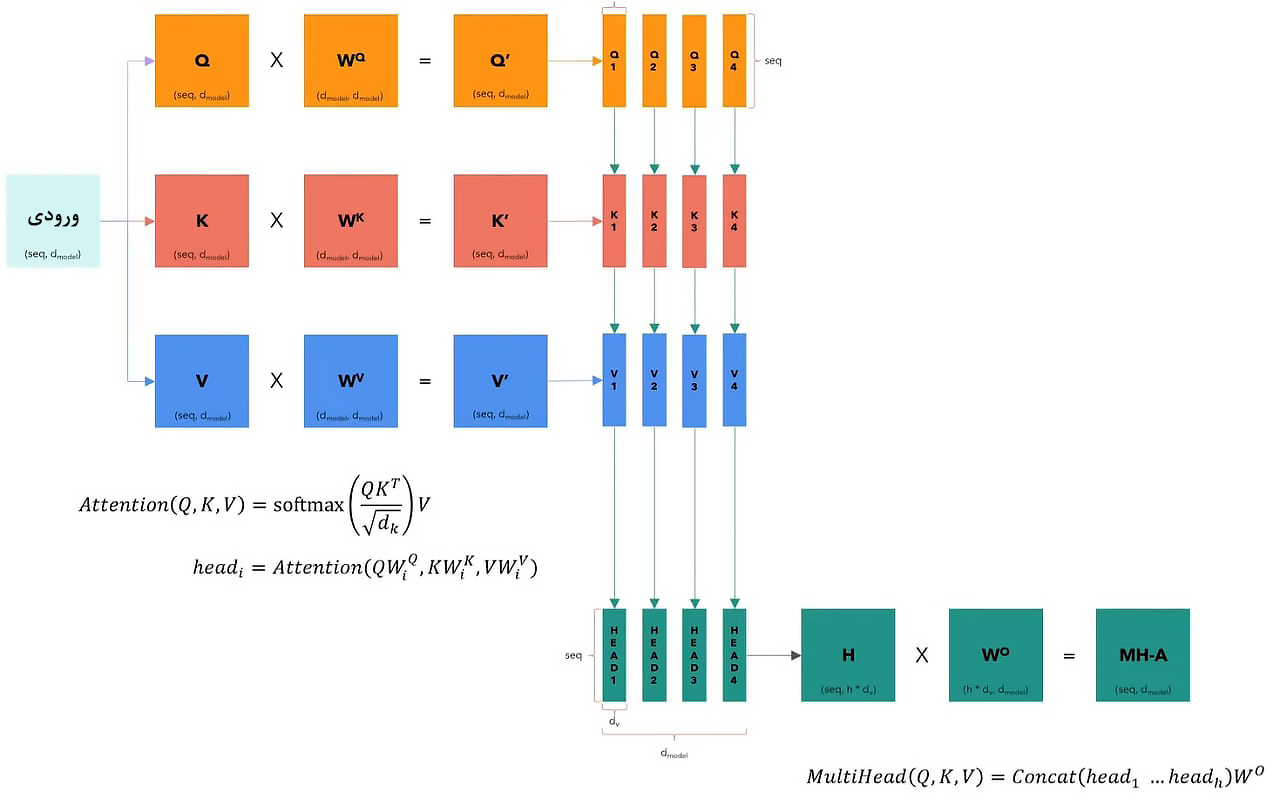
\includegraphics[width=\textwidth]{transformer_images/persian images/b01.png}
		\caption{توجه چند سر}
		\label{fig:attention}
	\end{minipage}
	\hfill
	
\end{figure}



\subsection*{چرا چندین سر؟}

\textbf{مشاهدهٔ چند منظر متفاوت:} هر  سر می‌تواند الگوهای گوناگونی از وابستگی‌ها را بیاموزد (مثلاً یک سر می‌تواند یاد بگیرد کلمهٔ فعلی با کلمات همسایهٔ نزدیک خود بیشتر مرتبط شود، یک سر  دیگر روی ارتباط با کلماتی در فاصلهٔ دورتری متمرکز باشد، سر دیگر روی مطابقت جنس و تعداد در دستور زبان و ...).

\textbf{افزایش ظرفیت مدل:} با داشتن چند سر ، مدل می‌تواند قدرت بیان بیشتری داشته باشد.

\textbf{ابعاد کمتر در هر سر:} در عمل، اگر \( d_{\text{model}} \) مثلاً 512 باشد، و تعداد سر ها \( h = 8 \)، آنگاه هر سر  ابعادی در حدود \( d_k = 64 \) خواهد داشت؛ و این محاسبات ضرب داخلی را نیز مقیاس‌ پذیر و قابل موازی‌سازی می‌کند.


\subsection{اتصال باقی مانده}
در معماری‌های عمیق، هنگامی که تعداد لایه‌ها زیاد می‌شود، اغلب دچار ناپایداری گرادیان می‌شوند و این مشکل باعث دشواری در آموزش مدل می‌گردد \cite{hochreiter1997long,bengio1994learning}. 

در مبدل ها \cite{vaswani2017attention}، به جای این که خروجی توجه را به‌صورت مستقیم به لایهٔ بعدی بدهیم، ورودی آن را نیز حفظ کرده و به خروجی اضافه می‌کنیم. ایدهٔ اصلی این روش از اتصالات باقی‌مانده \footnote{\lr{Residual Connection}} در شبکه‌های عمیق الهام گرفته شده است \cite{he2016deep}.

اگر \( x \) ورودی به زیرماژول و \( \text{SubLayer}(x) \) خروجی آن زیرماژول باشد، در انتهای کار عبارت زیر را محاسبه می‌کنیم:

\begin{equation}
	x + \text{SubLayer}(x)
	\label{eq:sublayer}
\end{equation}

این جمع به‌صورت عنصر به‌عنصر \footnote{\lr{Element-wise Addition}} انجام می‌شود.


اتصال باقیمانده در مبدل ها چندین مزیت دارد که عبارت اند از:

\subsection*{کمک به جریان یافتن گرادیان}
وقتی ورودی مستقیماً به خروجی اضافه می‌شود، مسیری مستقیم برای عبور شیب (گرادیان) به عقب ایجاد می‌گردد.
در صورت نبود این اتصال، اگر شبکه عمیق شود، گرادیان‌ها ممکن است در لایه‌های پایین محو شوند و عملاً ناپدید شدن گرادیان \footnote{\lr{gradient vanishing}} رخ دهد \cite{hochreiter1997long,bengio1994learning}.

\subsection*{حفظ اطلاعات اصلی (هویت ورودی)}
حتی اگر زیرماژول تغییری در اطلاعات ورودی ایجاد کند، با وجود اتصال باقیمانده \footnote{\lr{Residual Connection}}، ورودی اصلی همواره در خروجی نهایی حضور دارد.
این ویژگی باعث می‌شود در صورت ناکافی‌بودن یادگیری زیرماژول یا در مراحل اولیهٔ آموزش، دست‌کم بخشی از سیگنال (اطلاعات) خام به لایه‌های بالاتر برسد \cite{he2016deep,vaswani2017attention}.

\subsection*{کاهش ریسک تخریب ویژگی‌ها}
در شبکه‌های عمیق، یکی از مشکلات این است که هر لایه ممکن است بخشی از اطلاعات مفید را تخریب کند. اتصال باقی مانده تضمین می‌کند که اگر لایه‌ای به هر دلیل نتوانست الگوی بهینه را یاد بگیرد، اطلاعات قبلی حداقل به‌صورت دست‌نخورده تا حدی منتقل می‌شود.


\section{نرمال سازی لایه ها}

در یادگیری عمیق، نرمال‌سازی \footnote{\lr{Normalization}} داده‌های یک لایه یا فعال‌سازی‌ها، اغلب به سرعت بخشیدن به همگرایی و پایدار کردن آموزش کمک شایانی می‌کند. شاید معروف‌ترین نوع نرمال‌سازی، نرمال سازی بچ \footnote{\lr{Batch Normalization}} باشد که پیش‌تر در کارهای بینایی کانولوشنی\footnote{\lr{CNN}} بسیار مورداستفاده قرار گرفت \cite{ioffe2015batch}.

نرمال سازی لایه ها \footnote{\lr{Layer Normalization}} روشی جایگزین است که در ترانسفورمر استفاده می‌شود \cite{ba2016layer,vaswani2017attention}. علت اصلی این انتخاب، ماهیت توالی‌محور \footnote{\lr{sequence}} بودن داده‌ها در پردازش زبان طبیعی و عدم تمایل به وابستگی به آمار مینی‌بچ \footnote{\lr{mini-batch}} است.


\subsection*{نرمال سازی بچ}
در نرمال سازی بچ ها، برای نرمال‌سازی، میانگین و واریانس روی تمام نمونه‌های موجود در مینی‌بچ (و نیز در طول ابعاد ویژگی) محاسبه می‌شود \cite{ioffe2015batch}.
این موضوع در پردازش زبان طبیعی کمی دردسرساز است؛ چون ترتیب توکن‌ها، طول جمله‌ها و حتی اندازهٔ مینی‌بچ ممکن است نامنظم باشد.
همچنین به خاطر تنوع طول توالی‌ها، پیاده‌سازی نرمال سازی بچ ها می‌تواند پیچیده شود.

\subsection*{نرمال سازی لایه ها}
در  نرمال سازی لایه ها، برای هر توکن به‌صورت جداگانه (در طول بُعد ویژگی)، میانگین \footnote{\lr{mean}} و واریانس \footnote{\lr{variance}} گرفته می‌شود \cite{ba2016layer}.
فرض کنید در یک لایه، بردار \( h_i \in \mathbb{R}^{d_{\text{model}}} \) مربوط به توکن \( i \) باشد؛ یعنی ابعاد ویژگی آن \( d_{\text{model}} \) است. ما میانگین \( \mu_i \) و واریانس \( \sigma_i^2 \) را از اجزای این بردار محاسبه می‌کنیم:

\begin{equation}
	\mu_i = \frac{1}{d_{\text{model}}} \sum_{k=1}^{d_{\text{model}}} h_{i,k}, \quad
	\sigma_i^2 = \frac{1}{d_{\text{model}}} \sum_{k=1}^{d_{\text{model}}} (h_{i,k} - \mu_i)^2
	\label{eq:mean_variance}
\end{equation}


سپس نرمال‌سازی برای هر مؤلفهٔ \( k \) در بردار توکن \( i \) به شکل زیر انجام می‌شود:

\begin{equation}
	\hat{h}_{i,k} = \frac{h_{i,k} - \mu_i}{\sqrt{\sigma_i^2 + \epsilon}}
	\label{eq:normalized_h}
\end{equation}

در نهایت، برای این‌که مدل بتواند مقیاس و بایاس جدیدی یاد بگیرد، شبیه بچ نرم ، دو پارامتر \( \gamma \) و \( \beta \) نیز در طول بعد ویژگی اعمال می‌شوند:

\begin{equation}
	\text{LayerNorm}(h_i) = \gamma \odot \hat{h}_i + \beta
	\label{eq:layernorm}
\end{equation}


که در آن \( \gamma, \beta \in \mathbb{R}^{d_{\text{model}}} \) هستند و \( \odot \) ضربِ عنصر به عنصر است \cite{ba2016layer}.

\subsection*{مزایای نرمال سازی لایه در مبدل ها}

\begin{itemize}
	\item \textbf{بی‌نیازی از وابستگی به ابعاد مینی‌بچ:}  
	با نرمال سازی لایه، می‌توان حتی با اندازهٔ مینی‌بچ برابر ۱ نیز به‌خوبی آموزش دید، چراکه آمارها وابسته به ابعاد ویژگی‌اند و نه مینی‌بچ \cite{ba2016layer}.
	
	\item \textbf{پایدارسازی توزیع فعال‌سازی‌ها:}  
	زمانی که مدل در حال یادگیری است، توزیع‌های داخلی لایه‌های میانی ممکن است تغییر کند.\footnote{\lr{Internal Covariate Shift}} نرمال سازی لایه با نرمال‌سازی این توزیع، آموزش را پایدارتر و سریع‌تر می‌کند \cite{ioffe2015batch,ba2016layer}.
	
	\item \textbf{سازگاری با داده‌های توالی‌محور:}  
	هر توکن را جداگانه نرمال می‌کند و نگرانی‌ای بابت ترتیب طول جمله‌ها، یا قرار گرفتن چند جملهٔ کوتاه/بلند در یک مینی‌بچ نداریم \cite{vaswani2017attention}.
\end{itemize}

در معماری مبدل ها، پس از خروجی هر زیرماژول، مراحل به‌شکل زیر است:

\subsection{اتصال باقی مانده}
ابتدا ورودی همان زیرماژول (مثلاً بردار \( x \)) را با خروجی زیرماژول (\( \text{SubLayer}(x) \)) جمع می‌کنیم. حاصل این جمع را می‌توان چنین نوشت:


\begin{equation}
	z = x + \text{SubLayer}(x)
\end{equation}


این \( z \) حالا ترکیبی از اطلاعات اصلی ورودی و اطلاعات یادگرفته‌شده توسط \lr{SubLayer} است.

\paragraph{نرمال سازی لایه}
سپس این بردار \( z \) را وارد لایهٔ \lr{LayerNorm} می‌کنیم.

\[
y = \text{LayerNorm}(z)
\]

خروجی نهایی را می‌توان به لایهٔ بعدی پاس داد یا به مرحلهٔ بعدی در همین لایه.

به‌عبارتی اگر بخواهیم در یک فرمول واحد بیان کنیم:

\[
\text{Add \& Norm} = \text{LayerNorm}\bigl(x + \text{SubLayer}(x)\bigr)
\]


\section{رمزگشا}
رمزگشا در معماری ترانسفورمرها وظیفهٔ تولید خروجی نهایی را بر عهده دارد. این خروجی معمولاً می‌تواند توالی هدف \footnote{\lr{Target Sequence}} باشد، مانند ترجمه یک جمله یا پیش‌بینی توکن‌های بعدی در یک توالی \cite{vaswani2017attention}. 

در این بخش، رمزگشا دو ورودی اصلی دارد:  
1. توالی هدف که معمولاً به‌صورت خودکار تولید می‌شود (مثلاً در ترجمهٔ ماشینی یا تولید متن)،  
2. نمایش اطلاعات کدشده که توسط انکودر تولید شده است و شامل ویژگی‌های استخراج‌شده از توالی ورودی می‌باشد.  

رمزگشا از این ورودی‌ها استفاده می‌کند تا به‌صورت گام‌به‌گام، خروجی نهایی خود را تولید کند \cite{bahdanau2014neural,sutskever2014sequence}.

همان‌طور که در شکل \ref{fig:Decoder} مشاهده می‌کنید،  رمز گشا دو ورودی دارد.

\begin{figure}[h]
	\centering
	\begin{minipage}[b]{0.31\textwidth}
		\centering
		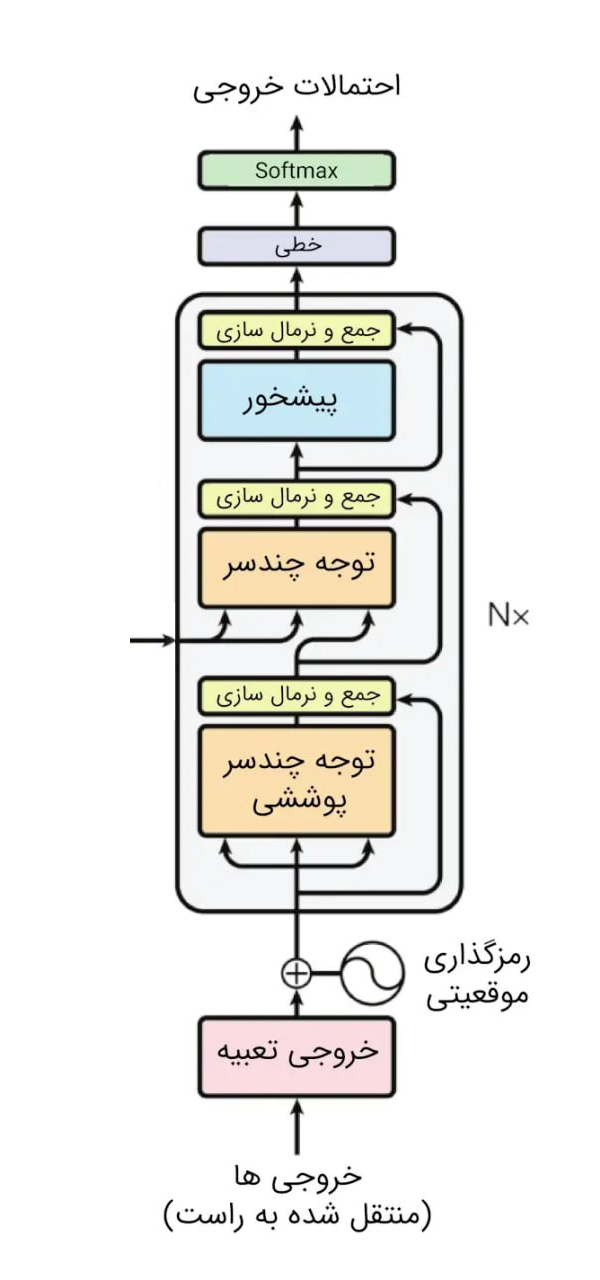
\includegraphics[width=\textwidth]{transformer_images/persian images/b06.png}
		\caption{رمزگشا در مبدل ها}
		\label{fig:Decoder}
	\end{minipage}
	\hfill
\end{figure}

تمامی بخش‌های رمزگشا مانند رمزگدار هستند اما در دیکودر توجه چند سر ماسک شده \footnote{\lr{Masked Multi-Head Attention}} وجود دارد \cite{vaswani2017attention}.



\section{توجه  چند سری ماسک شده}
در مبدل‌ها، مکانیزم توجه چند سری \footnote{\lr{Multi-Head Attention}} در بخش دیکودر به‌صورت ماسک شده \footnote{\lr{Masked}} پیاده‌سازی می‌شود تا مدل نتواند توکن‌های آینده را ببیند و به‌صورت خودبازگشتی \footnote{\lr{Autoregressive}} توکن بعدی را پیش‌بینی کند \cite{vaswani2017attention}.


در واقع ایده اصلی استفاده از ماسک جلوگیری از مشاهده آینده است.

در معماری‌های خودبازگشتی، مدل در گام \( i \) از دیکودر تنها باید به توکن‌های قبلی \( \{ y_1, \dots, y_{i-1} \} \) دسترسی داشته باشد؛ اما نه به توکن‌های \( \{ y_{i+1}, y_{i+2}, \dots \} \). اگر مدل بتواند توکن‌های آینده را «نگاه» کند، پیش‌بینی توکن بعدی آسان و غیرواقعی می‌شود (مشکل نشت اطلاعات) \cite{bahdanau2014neural,sutskever2014sequence}.

به همین دلیل در توجه چند سری ماسک شده در  دیکودر، از یک ماتریس ماسک \( M \) استفاده می‌کنیم که اجازه نمی‌دهد هر توکن به توکن‌های آینده‌اش توجه کند.

\section{مثال عددی توجه ماسک شده}
فرض کنید دنبالهٔ 4 توکنی داریم:
\[
[y_1, y_2, y_3, y_4]
\]
خروجی ضرب داخلی  (قبل از \texttt{softmax}) یک ماتریس \(4 \times 4\) خواهد بود:
\[
S =
\begin{bmatrix}
	s_{1,1} & s_{1,2} & s_{1,3} & s_{1,4} \\
	s_{2,1} & s_{2,2} & s_{2,3} & s_{2,4} \\
	s_{3,1} & s_{3,2} & s_{3,3} & s_{3,4} \\
	s_{4,1} & s_{4,2} & s_{4,3} & s_{4,4}
\end{bmatrix}
\]

\begin{itemize}
	\item \textbf{سطر 1 (توکن اول)}: تنها می‌تواند خودش (\textbf{ستون 1}) را ببیند، اما \textbf{ستون‌های 2 تا 4} ماسک می‌شوند.
	\item \textbf{سطر 2 (توکن دوم)}: می‌تواند به \textbf{ستون‌های 1 و 2} نگاه کند، اما \textbf{ستون‌های 3 و 4} ماسک می‌شوند.
	\item \textbf{سطر 3}: می‌تواند \textbf{ستون‌های 1، 2 و 3} را ببیند، اما \textbf{ستون 4} ماسک می‌شود.
	\item \textbf{سطر 4}: می‌تواند به \textbf{ستون‌های 1، 2، 3 و 4} دسترسی داشته باشد (چهارمین توکن می‌تواند توکن‌های قبلی را ببیند. همچنین این توکن \textbf{خودش} نیز معمولاً در دسترس است . بسته به پیاده‌سازی، ممکن است توکن فعلی از خودش نیز استفاده کند یا نه. در معماری استاندارد، سطر \( i \) معمولاً به ستون \( i \) هم دسترسی دارد).
\end{itemize}

در عمل، ماتریس ماسک \( M \) به شکل زیر خواهد بود (با نشانه‌گذاری پایین‌مثلثی):


\[
M =
\begin{bmatrix}
	0 & -\infty & -\infty & -\infty \\
	0 & 0 & -\infty & -\infty \\
	0 & 0 & 0 & -\infty \\
	0 & 0 & 0 & 0
\end{bmatrix}
\]

به این ترتیب، پس از جمع شدن با \( S \) و اجرای \texttt{softmax} در هر سطر، ضرایب توجه ستون‌های ماسک‌شده به صفر میل می‌کنند \cite{vaswani2017attention}.

 
\section{مبدل های بینایی}

ایده ترانسفورمرها در حوزهٔ بینایی \footnote{\lr{vision transformer}} از تعمیم ترانسفورمر متن به تصاویر به وجود آمده است \cite{dosovitskiy2020image}.

ما در این بخش از مبدل های بینایی برای وظیفه کلاس‌بندی استفاده می‌کنیم.

در روش‌های متداول برای پردازش تصویر، از کانولشن \footnote{\lr{convolution}} ‌های متوالی استفاده می‌کردند؛ اما در ترانسفورمرها تصاویر به پچ‌های مختلف شکسته می‌شوند \cite{dosovitskiy2020image}. هر پچِ شکسته‌شده از تصویر می‌تواند با سایر پچ‌ها به‌صورت موازی وارد مکانیزم توجه  شود و شباهت یا ارتباطشان با یکدیگر سنجیده شود. در بخش‌های بعد، به‌طور مفصل روند انجام این کار را توضیح خواهیم داد.


\subsection{جاسازی پچ ها در مبدل های بینایی}
در ترانسفورمرهای مبتنی بر متن، هر کلمه به توکن تبدیل می‌شود و سپس هر کلمه به برداری تبدیل می‌گردد. این بردارها پس از افزودن جاسازی موقعیتی وارد مکانیزم توجه می‌شوند \cite{vaswani2017attention}. 

حال همین ایده در تصویر پیاده‌سازی شده است. همان‌طور که در شکل \ref{fig:image to patch in vision transformer} مشاهده می‌کنید، در مبدل های بینایی، به‌جای استفاده از عملیات کانولوشن‌های متوالی که در شبکه‌های پیچشی \footnote{\lr{convolutional neural network}} مرسوم است \cite{lecun1998gradient,krizhevsky2012imagenet,he2016deep}، تصویر را به بلاک‌های غیرهم‌پوشان (\(P \times P\)) تقسیم می‌کنیم. این کار علاوه بر ساده‌سازی موازی‌سازی، به مدل اجازه می‌دهد از سازوکار توجه برای ارتباط بین این بلاک‌ها استفاده کند \cite{dosovitskiy2020image}.

\begin{figure}[h]
	\centering
	\begin{minipage}[b]{0.9\textwidth}
		\centering
		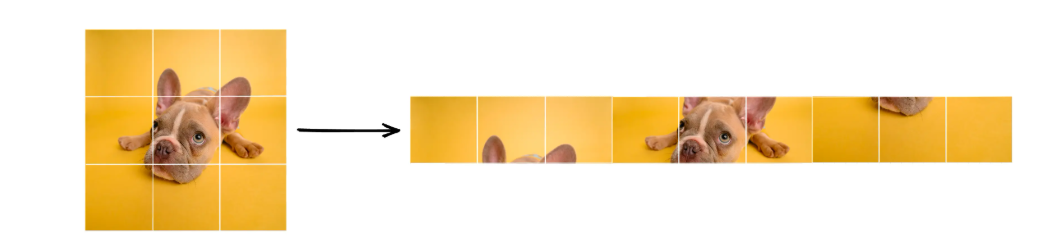
\includegraphics[width=\textwidth]{transformer_images/image_patch_embedding.png}
		\caption{بخش بندی تصاویر}
		\label{fig:image to patch in vision transformer}
	\end{minipage}
	\hfill
\end{figure}

\subsection{شکل پچ‌ها:}
فرض کنید ابعاد تصویر ورودی (\(H \times W \times C\)) باشد. به‌عنوان مثال، اگر اندازهٔ تصویر \(224 \times 224 \times 3\) باشد، طول و عرض تصویر به‌ترتیب \(224\) و تصویر دارای سه کانال رنگی است:

\[
H = 224, \quad W = 224, \quad C = 3
\]


حال اگر اندازهٔ هر پچ (\(P \times P\)) باشد (برای نمونه \(16 \times 16\))، تصویر به‌صورت یک جدول مشبک از پچ‌های کوچک تقسیم می‌شود.  
به هر پچ می‌توان مانند یک «کاشی» از تصویر نگاه کرد:
- پچ اول: مختصات \((0 \text{ تا } 15 \text{ در ارتفاع}) \) و \((0 \text{ تا } 15 \text{ در عرض})\)،  
- پچ دوم: مختصات \((0 \text{ تا } 15 \text{ در ارتفاع}) \) و \((16 \text{ تا } 31 \text{ در عرض})\)،  
- و به همین ترتیب تا کل تصویر پوشش داده شود.



\subsection{تعداد پچ‌ها:}
اگر پچ‌ها بدون هم‌پوشانی باشند، ابعاد پچ باید بر ابعاد تصویر بخش‌پذیر باشد.  

- تعداد پچ‌های افقی: \(\frac{W}{P}\)  
- تعداد پچ‌های عمودی: \(\frac{H}{P}\)  

در مجموع:  
\begin{equation}
	\left(\frac{H}{P}\right) \times \left(\frac{W}{P}\right) = \frac{H}{P} \times \frac{W}{P}.
	\label{eq:grid_size}
\end{equation}


برای مثال اگر:
\[
H = 224, \quad W = 224, \quad P = 16:
\]
\[
\frac{224}{16} = 14 \quad \Rightarrow \quad 14 \times 14 = 196 \quad (\text{تعداد پچ‌ها}).
\]

در اکثر نسخه‌های مبدل‌های بینایی، پچ‌ها بدون هم‌پوشانی \footnote{\lr{Non-overlapping}} هستند. اندازه پچ‌های کوچک باعث می‌شود تعداد پچ‌ها زیاد شود و در نتیجه هزینه توجه بالا رود. از طرفی، پچ‌های بزرگ هزینه توجه را کاهش می‌دهند؛ اما ممکن است جزییات محلی \footnote{\lr{Local Details}} را از دست بدهیم \cite{dosovitskiy2020image}.


\subsection{بردارکردن هر پچ}
هر پچ دارای ابعاد \((P \times P \times C)\) است. برای مثال اگر \(P=16\) و \(C=3\)، آنگاه پچ ابعاد \(16 \times 16 \times 3\) خواهد داشت.  
برای این‌که بتوانیم پچ‌ها را مانند «توکن»‌های پردازش زبان ظبیعی به مبدل ها بدهیم، باید آن‌ها را به یک بردار یک ‌بعدی تبدیل کنیم. در صورت قرار دادن پیکسل‌های پچ به‌صورت ردیفی \footnote{\lr{Row-major}}، طول این بردار خواهد بود:

\begin{equation}
	P \times P \times C = P^2 \times C.
	\label{eq:patch_volume}
\end{equation}

در مثال \((16 \times 16 \times 3)\)، طول بردار می‌شود \(768\).


\section{اعمال لایهٔ خطی}
بعد از کنار هم چیدن پچ ها \footnote{\lr{Flatten}}، معمولاً یک لایهٔ خطی \footnote{\lr{Fully-Connected Layer}} روی این بردار اعمال می‌شود تا آن را به بعد \(d_{\text{model}}\) (مثلاً 768 یا 1024) ببرد. در حقیقت، این لایه یک تبدیل ویژگی \footnote{\lr{Feature Transformation}} انجام می‌دهد تا همه پچ‌ها یک نمایندگی (تعبیه شده) با ابعاد یکنواخت \(d_{\text{model}}\) پیدا کنند:
\[
(P^2 \times C) \quad \rightarrow \quad d_{\text{model}}
\]

\begin{figure}[h]
	\centering
	\begin{minipage}[b]{0.9\textwidth}
		\centering
		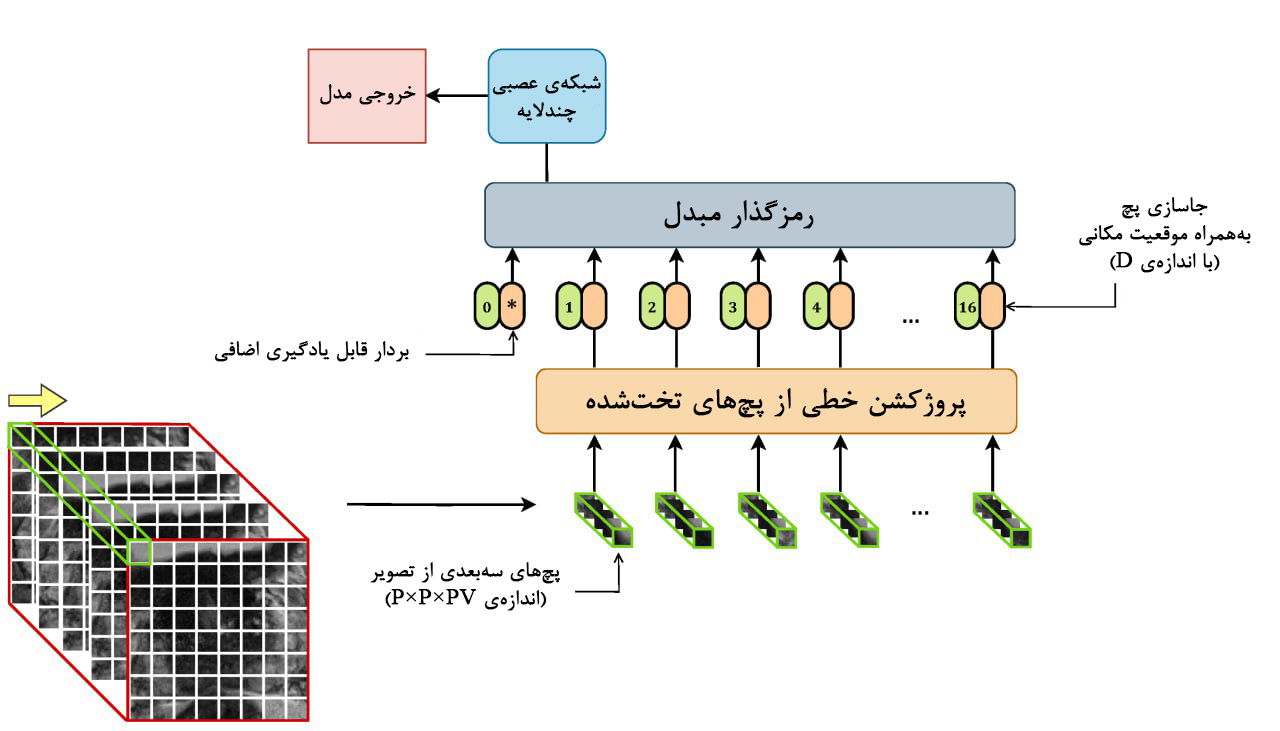
\includegraphics[width=\textwidth]{transformer_images/persian images/b07.png}
		\caption{مبدل های بینایی}
		\label{fig:Embedding Vision Transformer}
	\end{minipage}
	\hfill
\end{figure}

این مرحله شبیه ساخت توکن در پردازش زبان طبیعی است؛ با این تفاوت که در پردازش زبان طبیعی، توکن «کلمه» یا «زیرکلمه» است و از قبل دارای بردار تعبیه‌شده جاساز شده بوده است \cite{vaswani2017attention}. در مبدل های بینایی \cite{dosovitskiy2020image}، ما ابتدا باید تصاویر را پچ کنیم و سپس بردارهای  جاساز را از این پچ‌ها به دست آوریم.

ترانسفورمر نیاز دارد ورودی‌اش توالی توکن‌ها باشد. در پردازش زبان طبیعی توالی کلمات داریم، در مبدل های بینایی توالی «پچ»‌ها:
\[
\{ x_{\text{patch}_1}, x_{\text{patch}_2}, \dots, x_{\text{patch}_N} \}.
\]
هر پچ اکنون یک بردار \(d_{\text{model}}\)-بعدی است. پس یک مجموعه با طول \(N\) (تعداد پچ‌ها) و عرض \(d_{\text{model}}\) خواهیم داشت.  
اگر عدد پچ‌ها \(N\) باشد (مثلاً 196)، ترانسفورمر می‌تواند با مکانیزم توجه خود سر، وابستگی  میان پچ‌ها را یاد بگیرد: کدام بخش از تصویر برای کدام بخش دیگر مهم‌تر است\cite{vaswani2017attention,dosovitskiy2020image}.

معمولاً پچ‌ها را به‌صورت ردیفی شماره‌گذاری می‌کنند (ابتدا پچ‌های ردیف بالایی از چپ به راست، سپس ردیف بعدی و …)، تا مدل در صورت نیاز بتواند از موقعیت‌ها، اطلاعات مکانی تقریبی داشته باشد.  
در عمل، چون قصد داریم (در مراحل بعد) به هر پچ یک جاسازی موقعیتی هم اضافه کنیم، مکان دقیق هر پچ در بُعد دوم (ویژگی) کد می‌شود.

در مبدل بینایی \cite{dosovitskiy2020image} دیگر به کانولوشن وابسته نیستیم. در عوض، از جاسازی استفاده می‌شود.  
تقسیم  کردن تصویر به بلاک‌های \((P \times P)\)، کنار هم چیدن و تبدیل آن به جاساز همگی عملیات ریاضی ساده‌ای هستند که به‌راحتی روی \lr{GPU}/\lr{TPU} قابل موازی‌سازی‌اند.

\subsection{توکن کلاس بندی}
توکن کلاس بندی \footnote{\lr{Cls Token}} یک بردار ویژه است که به ابتدای دنبالهٔ ورودی اضافه می‌شود و نقش آن، خلاصه‌کردن اطلاعات کل ورودی (چه متن، چه تصویر) است \cite{devlin2018bert,dosovitskiy2020image}.

در مبدل بینایی، این توکن در ابتدای پچ‌های تصویری قرار می‌گیرد.  
این توکن یک بردار با ابعاد \(d_{\text{model}}\) است (همان ابعاد سایر توکن‌ها) و پارامتری یادگرفتنی محسوب می‌شود؛ یعنی مدل طی آموزش، مقادیر آن را برای ذخیره و تجمیع اطلاعات بهینه می‌کند.

در وظایف دسته‌بندی کلاس بندی، هدف این است که یک پیش‌بینی کلی برای کل ورودی (مثلاً یک جمله یا یک تصویر) ارائه دهیم؛ توکن کلاس بندی دقیقاً همین وظیفه را بر عهده دارد \cite{devlin2018bert}. این توکن از طریق مکانیزم توجه چند سر در مبدل ها با تمامی توکن‌های دیگر (پچ‌های تصویر) ارتباط می‌گیرد و اطلاعات مهم آن‌ها را در لایه‌های مختلف مبدل ها را به‌صورت تجمعی یاد می‌گیرد. به عبارتی، توکن کلاس بندی نقش نماینده کل تصویر یا متن را بر عهده دارد.

توکن کلاس بندی از طریق ضرب داخلی در مکانیزم توجه، می‌تواند به تمام پچ‌ها نگاه کند و با ضرایب توجه (\(\alpha\)) مشخص کند که از هر پچ چه مقدار اطلاعات بگیرد. بدین‌ترتیب، به‌طور ضمنی یاد می‌گیرد روی ویژگی‌هایی که برای دسته‌بندی مهم هستند (نظیر الگوها، اشکال و بخش‌های کلیدی تصویر) متمرکز شود.

در طول لایه‌های ترانسفورمر، توکن کلاس بندی نقش محوری در خلاصه‌سازی بازنمایی کل تصویر ایفا می‌کند. این توکن به‌صورت پارامتر قابل یادگیری تعریف شده و در طول فرآیند آموزش به‌روزرسانی می‌شود \cite{devlin2018bert,dosovitskiy2020image}.

\subsection{رمزگذار در مبدل های بینایی}

رمزگذار در ترانسفورمرها همانند مبدل اصلی است \cite{vaswani2017attention}، با این تفاوت که در مبدل های بینایی \cite{dosovitskiy2020image} دیگر به رمزگشا نمی‌رویم. پس از عبور از بلاک‌های ترانسفورمر، در ساده‌ترین حالت یک لایه خطی \footnote{\lr{Fully Connected}} یا یک لایه \lr{MLP} \footnote{\lr{Multi-Layer Perceptron}} بر روی بردار نهایی اعمال می‌شود و این لایه‌ها به تعداد کلاس‌ها خروجی می‌دهند.  
سپس خروجی هر لایه با گذر از تابع سافت مکس \footnote{\lr{softmax}} به احتمال هر کلاس تبدیل می‌شود و در نهایت مدل کلاس با بیشترین احتمال را به‌عنوان خروجی پیش‌بینی می‌کند.

\begin{figure}[h]
	\centering
	\begin{minipage}[b]{0.9\textwidth}
		\centering
		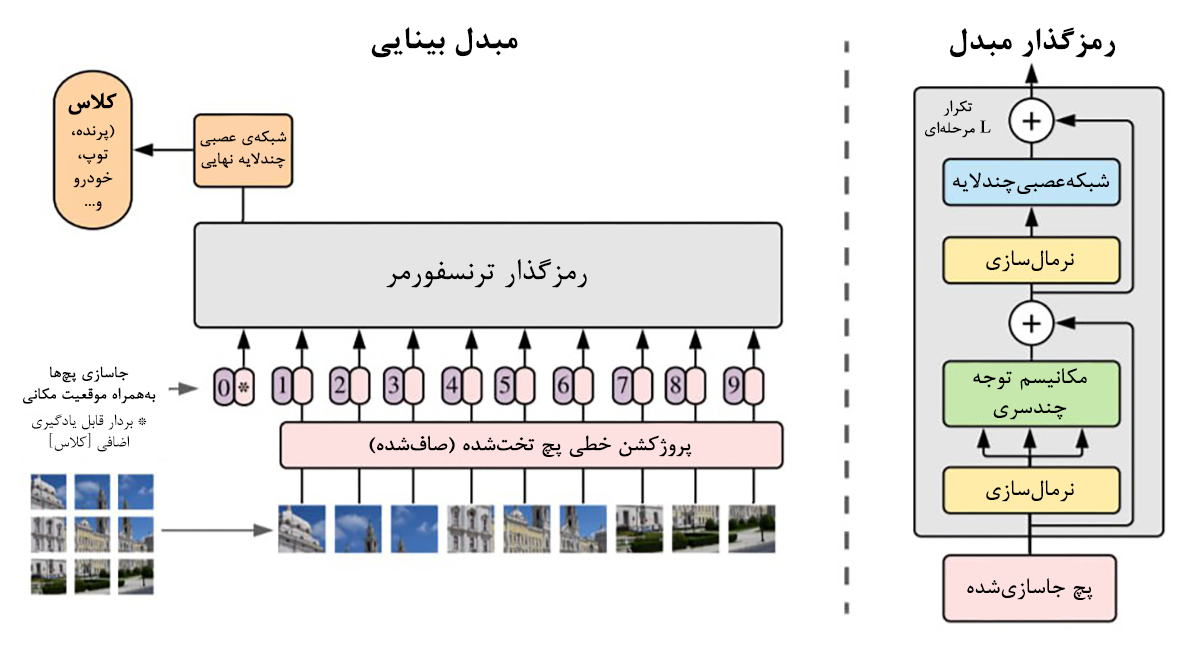
\includegraphics[width=\textwidth]{transformer_images/persian images/persian_images/b08.png}
		\caption{توکن توجه در مبدل های بینایی}
		\label{fig:Cls Token In Vision Transformer}
	\end{minipage}
	\hfill
\end{figure}

در مبدل ها، هر لایه رمزگشا و رمزگذار با پردازش عمیق‌تر روی توالی ورودی، می‌تواند نمایش بهتری از ویژگی‌ها به‌دست بیاورد \cite{vaswani2017attention}. تکرار چندین‌باره رمزگشا یا رمزگذار موجب می‌شود مدل بتواند ساختارهای پیچیده‌ای را یاد بگیرد و کیفیت و دقت آن در شناسایی توالی‌های طولانی و معانی پنهان افزایش یابد \cite{vaswani2017attention,dosovitskiy2020image}. 
در نتیجه، مدل با تعداد لایه‌های بیشتر اغلب عملکرد بهتری از خود نشان می‌دهد.

   
   
\section{مبدل پنجره‌ای متحرک}
ایده مبدل پنجره‌ای متحرک \footnote{\lr{Swin Transformer}} از ترکیب چند مفهوم کلیدی در مدل‌های ترانسفورمر و شبکه‌های پیچشی شکل گرفت \cite{vaswani2017attention,he2016deep,liu2021swintransformer}.

یکی از بزرگترین مشکلات در ترانسفورمرهای اولیه، نیاز به محاسبات بسیار زیاد در زمانی بود که تصویر ورودی ابعاد بسیار بزرگی داشت \cite{dosovitskiy2020image}. در ترانسفورمر معمولی هر پچ به تمامی پچ‌های دیگر توجه  می‌کرد و در مواقعی که تعداد پچ‌ها زیاد می‌شد، هزینه محاسباتی و حافظه به‌شدت افزایش پیدا می‌کرد.

در شبکه‌های پیچشی، معماری معمولاً به‌صورت سلسله‌مراتبی پیش می‌رود \cite{he2016deep}؛ یعنی ابتدا ویژگی‌های محلی استخراج می‌شود، سپس با عمیق‌تر شدن لایه‌ها، این ویژگی‌ها در سطوح بالاتر با یکدیگر ترکیب می‌شوند. در مبدل پنجره‌ای متحرک \cite{liu2021swintransformer}، با دانش بر این موضوع توانسته‌اند هم هزینه‌های محاسباتی را کاهش دهند و هم دقت مدل را افزایش دهند.

\begin{figure}[h]
	\centering
	\begin{minipage}[b]{1\textwidth}
		\centering
		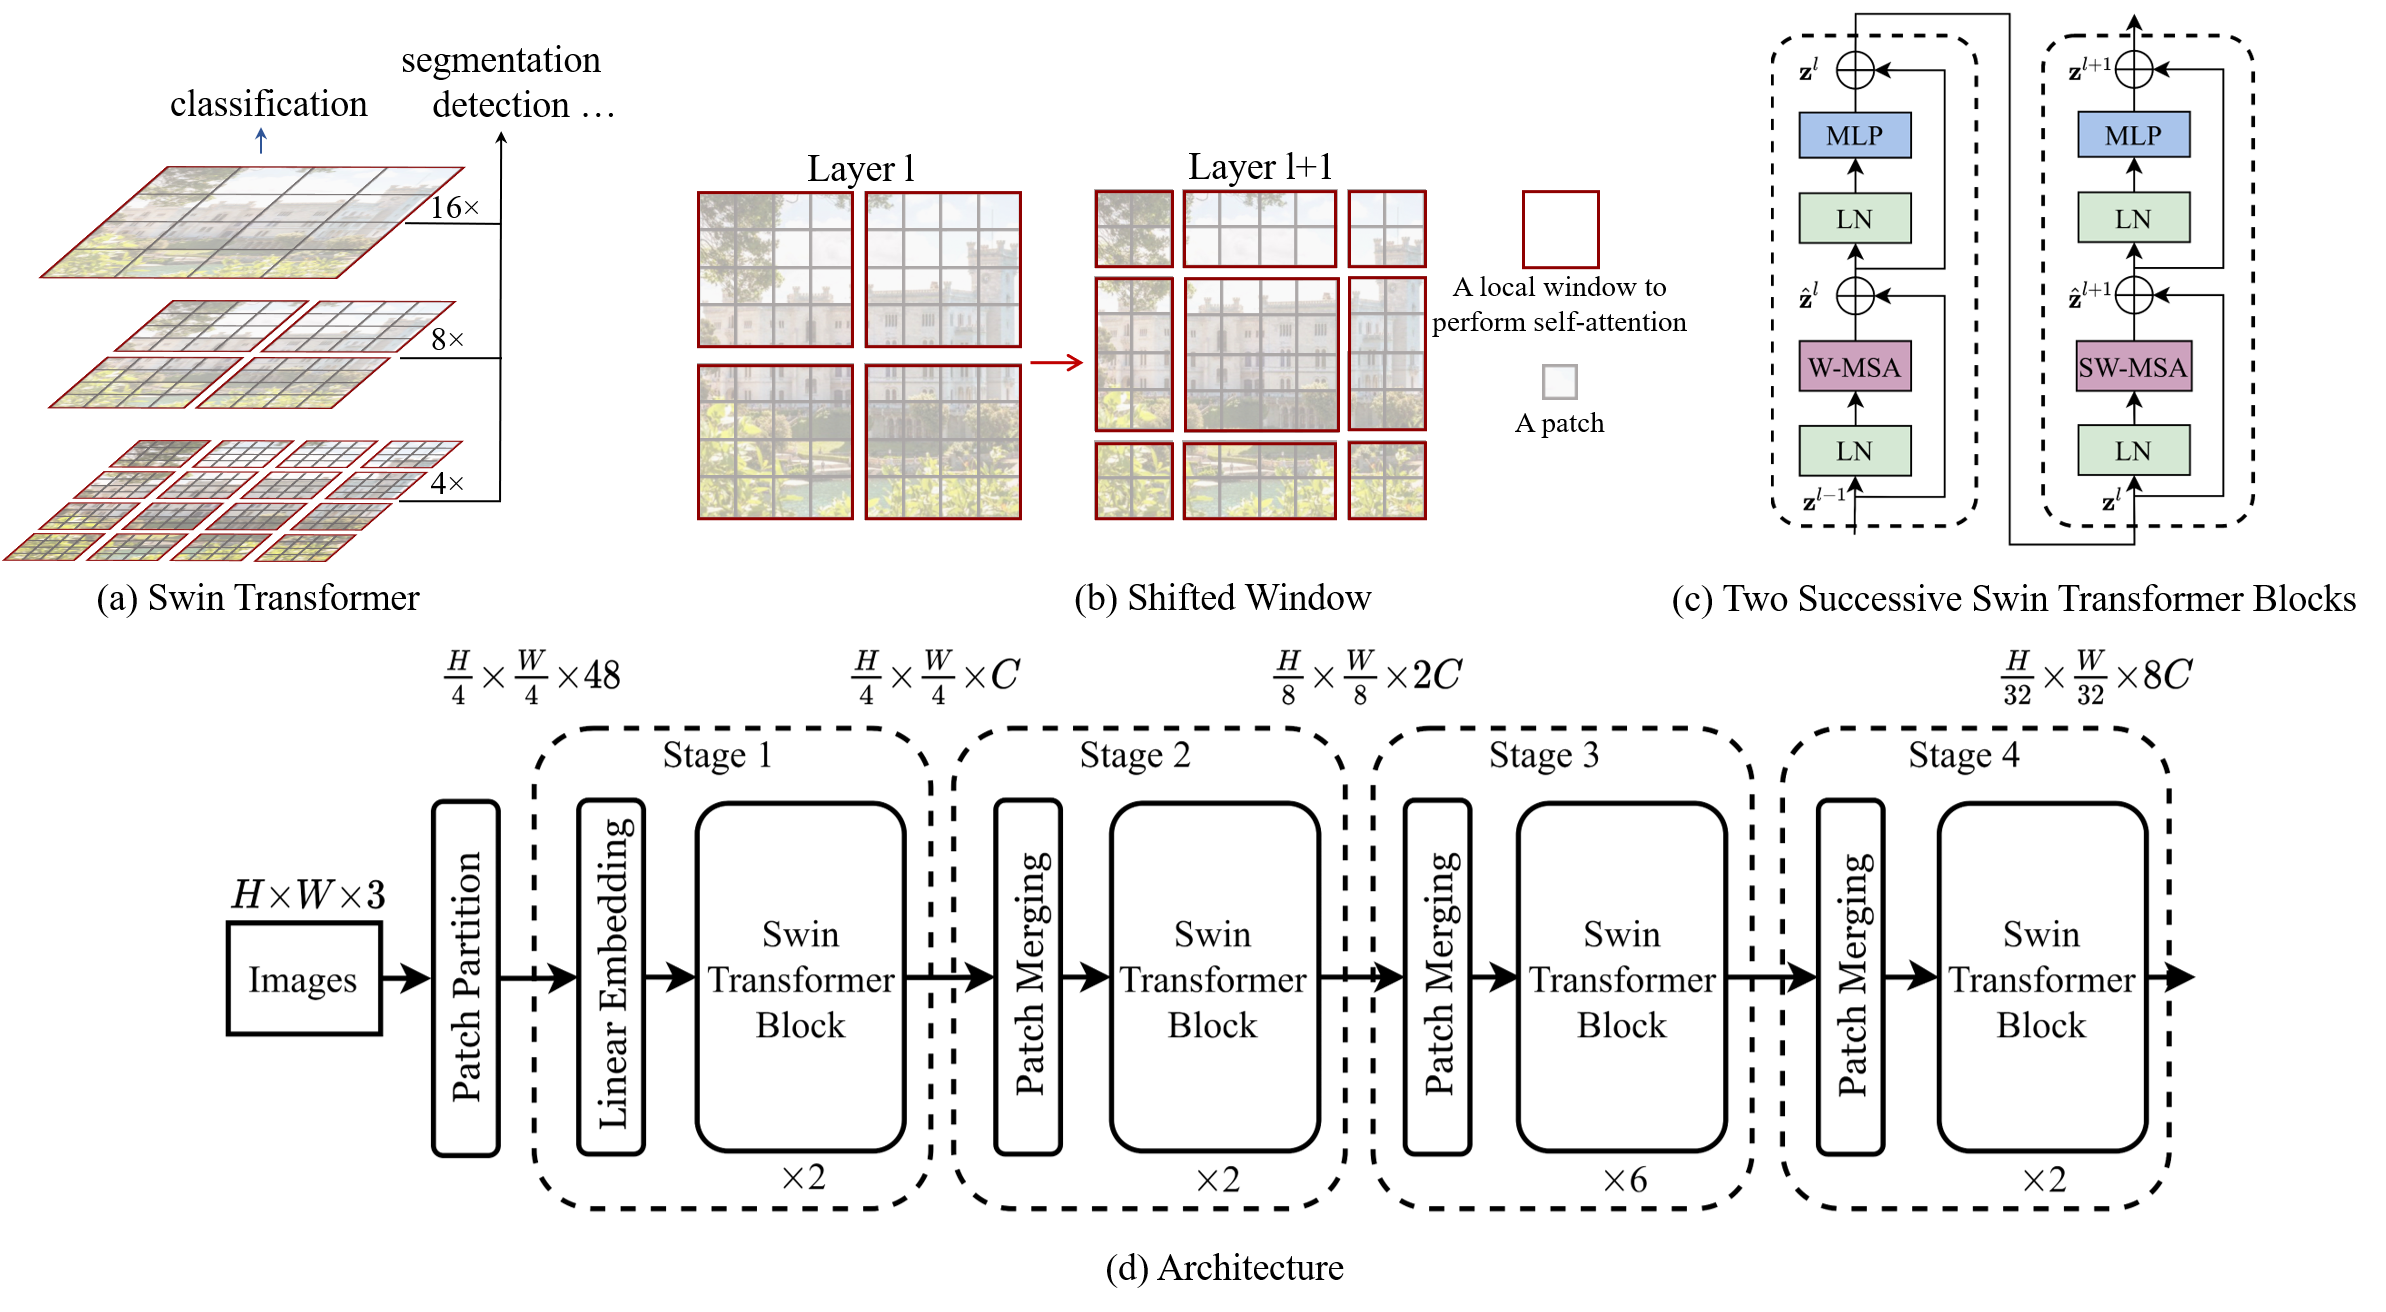
\includegraphics[width=\textwidth]{transformer_images/swin_transformer.png}
		\caption{مبدل پنجره متحرک}
		\label{fig: swin transformer}
	\end{minipage}
	\hfill
\end{figure}

در مبدل پنجره‌ای متحرک، به‌جای آن‌که مدل به تمام پچ‌ها در یک سطح ویژگی نگاه کند، تصویر را به «پنجره‌های محلی» \footnote{\lr{Local Windows}} تقسیم می‌کند و توجه را محدود به همان ناحیه می‌سازد \cite{liu2021swintransformer}. سپس با تکنیک جابه‌جایی \footnote{\lr{Shift}} این پنجره‌ها در لایه‌های بعدی، توان مدل برای ترکیب اطلاعات از نواحی مختلف تصویر (و در نهایت دیدن کل تصویر) افزایش پیدا می‌کند. این رویکرد، ایدهٔ کلیدی‌ای بود که باعث شد مدل هم محاسبات سبک‌تری داشته باشد و هم بتواند ارتباط‌های جهانی \footnote{\lr{Global}} را در طول لایه‌ها به‌دست آورد.



یکی دیگر از ایده‌های مهم در در مبدل پنجره‌ای متحرک، کوچک‌ کردن تدریجی نقشهٔ ویژگی  در طول معماری است؛ مشابه کاری که در \lr{ResNet} یا سایر \lr{CNN}ها انجام می‌شود \cite{he2016deep}. این امر ضمن کاهش هزینه محاسباتی، باعث می‌شود مدل بتواند با سطوح مختلفی از ویژگی‌ها کار کند و در نهایت خروجی نهایی باکیفیت‌تری ارائه دهد.

\subsection{قطعه‌بندی پچ در مبدل پنجره متحرک}
فرض کنیم تصویر ورودی \(\displaystyle I\) دارای ابعاد \(\displaystyle (H \times W \times 3)\) باشد. گام نخست، تقسیم تصویر به پچ‌های کوچک \(\displaystyle (P \times P)\) است \cite{dosovitskiy2020image}. اگر \(P\) اندازهٔ پچ \footnote{\lr{patch size}} باشد، آنگاه تعداد پچ‌ها در بعد افقی و عمودی، به‌ترتیب \(\displaystyle \frac{H}{P}\) و \(\displaystyle \frac{W}{P}\) خواهد بود. هر پچ را می‌توان به‌صورت یک بردار درآورد:

\[
X_{\text{patch}} \in \mathbb{R}^{(P^2 \cdot 3)}.
\]

سپس کل تصویر به \(\displaystyle \frac{H}{P} \times \frac{W}{P}\) پچ تبدیل خواهد شد و در نتیجه، ماتریس \(\displaystyle X\) از کنار هم قرار گرفتن این پچ‌ها به صورت زیر به‌دست می‌آید:

\[
X \in \mathbb{R}^{\Bigl(\frac{H}{P} \cdot \frac{W}{P}\Bigr) \times \Bigl(P^2 \cdot 3\Bigr)}.
\]

برخلاف مبدل بینایی اصلی این کاردر مبدل پنجره متحرک با استفاده از کانولوشن \footnote{\lr{convolution}} انجام می شود.
در واقع سایز کرنل در کانولوشن همان فضای برداری هر پچ هست که ما فرض میکنیم سایز کرنل برابر c ‌است. پس درنتیجه



\begin{equation}
	Z = X \cdot W_{\text{embed}} + b_{\text{embed}}, 
	\quad
	Z \in \mathbb{R}^{\Bigl(\tfrac{H}{P} \cdot \tfrac{W}{P}\Bigr) \times C}.
\end{equation}

در عمل، این عملیات معادل یک تبدیل خطی ساده است:

\[
W_{\text{embed}} \in \mathbb{R}^{\bigl(P^2 \cdot 3\bigr) \times C},
\quad
b_{\text{embed}} \in \mathbb{R}^{C}.
\]

پس از این مرحله، ما در هر موقعیت \((h, w)\) (از شبکهٔ پچ‌ها) یک بردار 
\(\displaystyle z_{h,w} \in \mathbb{R}^{C}\) داریم. این ماتریس \(\displaystyle Z\) 
ورودیِ اولین مرحله (\lr{Stage}) از مبدل های پنجره متحرک خواهد بود \cite{liu2021swintransformer}.

هر بلوک مبدل پنجره متحرک از چند بخش اصلی تشکیل شده است \cite{liu2021swintransformer}:

\begin{itemize}
	\item پنجره‌بندی تصویر \footnote{\lr{Window Partition}} 
	یا پنجره‌بندی جابه‌جاشده \footnote{\lr{Shifted Window Partition}}
	\item اعمال توجه چمد سر پنجره ای \footnote{\lr{Window Multi-Head Self Attention}}
	\item لایهٔ \lr{Skip Connection}\footnote{\lr{Skip Connection}} و \lr{Layer Norm}\footnote{\lr{Layer Norm}}
	\item مسیر پرسیپترون چندلایه \footnote{\lr{MLP}}:
% 	\begin{itemize}
% 			\item یک لایهٔ \lr{MLP} شامل دو لایهٔ \lr{Fully-Connected}\footnote{\lr{Fully-Connected}} 
	% 		و تابع فعال‌ساز \lr{GeLU}\footnote{\lr{GeLU}} % 	(یا تابع مشابه)
% 			\item لایهٔ \lr{Skip Connection}\footnote{\lr{Skip Connection}} و \lr{Layer Norm}\footnote{\lr{Layer Norm}}
% 	\end{itemize}
\end{itemize}




\subsection{توجه چند سر پنجره ای}

\subsubsection{تعریف پنجره‌های محلی}

در مبدل های پنجره متحرک، به‌جای آن‌که تمام پیکسل‌های یک نقشهٔ ویژگی بزرگ را یک‌جا 
در محاسبهٔ توجه  درگیر کنیم، نقشهٔ ویژگی را به قطعه‌های کوچکی به‌اندازه
\(\displaystyle (M \times M)\) تقسیم می‌کنیم. این قطعه‌های کوچک را 
«پنجره‌های محلی» می‌نامیم.

اگر اندازهٔ نقشهٔ ویژگی در یک لایه 
\(\displaystyle (H' \times W')\) باشد، 
با تقسیم آن به پنجره‌های 
\(\displaystyle (M \times M)\)، 
در راستای طول تقریباً 
\(\displaystyle \tfrac{H'}{M}\) پنجره خواهیم داشت 
و در راستای عرض هم 
\(\displaystyle \tfrac{W'}{M}\) پنجره.
(برای راحتی، فرض می‌کنیم 
\(\displaystyle H'\) و \(\displaystyle W'\) 
دقیقاً مضربی از \(\displaystyle M\) باشند 
تا تقسیم بدون باقی‌مانده انجام شود.)

هر کدام از این پنجره‌های 
\(\displaystyle (M \times M)\) 
دارای 
\(\displaystyle M^2\) پیکسل (یا موقعیت مکانی) است، 
و در هر پیکسل هم یک بردار ویژگی با بعد \(\displaystyle C\) قرار دارد.

به بیان ساده‌تر:
\begin{itemize}
	\item نقشهٔ ویژگی مثل یک صفحهٔ بزرگ است.
	\item آن را مانند شطرنج به مربع‌های کوچکی \(\displaystyle (M \times M)\) بخش می‌کنیم.
	\item در هر مربع (پنجره)، فقط به همان مربع نگاه می‌کنیم و محاسبات  توجه  را انجام می‌دهیم.
	\item این کار باعث می‌شود تعداد پیکسل‌هایی که درگیر محاسبهٔ توجه هستند، 
	به‌مراتب کمتر شود و هزینهٔ محاسباتی کاهش یابد.
\end{itemize}


\subsection{توجه}

برای هر بلوک، ابتدا بردارهای پرسش، کلید، مقدار ساخته می‌شوند. 
اگر \(\displaystyle z_i \in \mathbb{R}^C\) بردار ورودی مربوط به موقعیت \(i\) باشد، آنگاه:


\begin{equation}
	q_i = z_i W_Q, 
	\quad
	k_i = z_i W_K,
	\quad
	v_i = z_i W_V,
\end{equation}

	که 

\[
W_Q, W_K, W_V \;\;\in \;\;\mathbb{R}^{C \times d}.
\]

پارامتر \(\displaystyle d\) معمولاً به‌صورت \(\displaystyle \tfrac{C}{h}\) در نظر گرفته می‌شود 
که در آن \(\displaystyle h\) تعداد سربندی  سر ها است. 
در توجه چند سر، خروجی نهایی با ترکیب \(\displaystyle h\) سر توجه محاسبه می‌شود.

در یک سر توجه، توجه به‌صورت زیر تعریف می‌شود:

\begin{equation}
	\mathrm{Attention}(Q, K, V)
	=
	\mathrm{Softmax}\Bigl(\frac{QK^\top}{\sqrt{d}}\Bigr)\,V,
\end{equation}

که در آن:

\begin{itemize}
	\item \(\displaystyle Q, K, V\) به‌ترتیب ماتریس‌هایی هستند که از کنار هم قرار دادن 
	\(\displaystyle q_i, k_i, v_i\) (برای تمام پیکسل‌های آن پنجره) ساخته می‌شوند.
	\item \(\displaystyle \sqrt{d}\): عامل مقیاس‌کننده برای جلوگیری از بزرگ شدن بیش‌ازحد ضرب داخلی است.
\end{itemize}

در مبدل های پنجره متحرک، این محاسبات به‌صورت پنجره‌ای انجام می‌شوند؛ یعنی 
برای هر پنجره، تنها پیکسل‌های داخل همان پنجره در ماتریس‌های 
\(\displaystyle Q\)، \(\displaystyle K\) و \(\displaystyle V\) لحاظ می‌شوند. 
به این ترتیب، زمان محاسبه و مصرف حافظه به‌شدت کاهش می‌یابد 
(در مقایسه با مبدل های بینایی که همه‌چیز را با هم مقایسه می‌کند).

تعداد سربندی \(\displaystyle h\) معمولاً طوری انتخاب می‌شود که 
\(\displaystyle C = h \times d.\) 
خروجی هر سر پس از محاسبه توجه به‌صورت زیر با هم ادغام می‌شوند:

\begin{equation}
	\mathrm{MultiHead}(Q,K,V) 
	= 
	\bigl[\text{head}_1,\ \text{head}_2,\ \dots,\ \text{head}_h\bigr]\,
	W_O,
\end{equation}

که 
\[
\text{head}_j = \mathrm{Attention}\bigl(Q_j,\ K_j,\ V_j\bigr),
\quad 
W_O \in \mathbb{R}^{C \times C}
\]
ماتریس ترکیب نهایی است.

\subsection{پنجره متحرک جا به جا شده}

در مدبل های پنجر متحرک، ایدهٔ «پنجره‌های جابه‌جاشده»    \footnote{\lr{Shifted Windows}}
به این منظور ارائه شده است تا مدل، ارتباط پیکسل‌های واقع در پنجره‌های مجاور را هم یاد بگیرد \cite{liu2021swintransformer}.
اگر فقط از پنجره‌های ثابت (بدون جابه‌جایی) استفاده کنیم، هر بلوک از تصویر تنها با پیکسل‌های همان 
پنجره در ارتباط خواهد بود و ممکن است اطلاعات نواحی مرزی با نواحی مجاور به‌خوبی تبادل نشود.

روش مبدل های پنجره متحرک برای رفع این محدودیت از یک تکنیک ساده اما مؤثر استفاده می‌کند \cite{liu2021swintransformer}:
\begin{itemize}
	\item در یک لایه، محاسبات توجه در پنجره‌های محلی ثابت انجام می‌شود.
	\item در لایهٔ بعدی، پنجره‌ها به اندازه‌ای مشخص جابه‌جا می‌شوند (به‌صورت شیفت افقی و عمودی) 
	تا نواحی مرزی نیز در محاسبات گنجانده شوند.
	\item این فرآیند باعث می‌شود که پیکسل‌ها در پنجره‌های مختلف (و در مرزهای مختلف) 
	در محاسبات دخیل شوند و تبادل اطلاعات بهتری میان نواحی تصویر رخ دهد.
\end{itemize}

\subsubsection{توجه چند سری پنجره ای}
در توجه چندسری پنجره ای \footnote{\lr{W-MSA}}، نقشهٔ ویژگی به پنجره‌های \(\displaystyle (M \times M)\) تقسیم می‌شود \cite{liu2021swintransformer}.
هیچ جابه‌جایی در این تقسیم‌بندی وجود ندارد؛ یعنی اگر نقشهٔ ویژگی را یک مستطیل بزرگ در نظر بگیریم،
آن را شبیه کاشی‌کاری یا شطرنج‌بندی به بلوک‌های مربعی \(\displaystyle (M \times M)\) برش می‌زنیم.
در این حالت، پیکسل‌های هر پنجره فقط با همدیگر (درون همان پنجره) ارتباط برقرار می‌کنند.

\subsubsection{توجه چند سری پنجره ای جا به جا شده}
مطابق شکل \ref{fig:Cycle Shift in Swin Tranformer}، بعد از اینکه بلوک اول (توجه چند سری پنجره ای) کارش تمام شد، در بلوک دوم، قبل از تقسیم‌بندی به پنجره‌های 
\(\displaystyle (M \times M)\)، نقشهٔ ویژگی را جابه‌جا  می‌کنیم \cite{liu2021swintransformer}.
در مقالهٔ اصلی، این مقدار جابه‌جایی معمولاً نیمِ اندازهٔ پنجره 
\(\displaystyle \frac{M}{2}\)
در راستای افقی و عمودی است. به این ترتیب:

\begin{itemize}
	\item پیکسل‌هایی که پیش از این در دو پنجرهٔ جداگانه قرار داشتند، ممکن است حالا به دلیل جابه‌جایی وارد یک پنجرهٔ مشترک شوند.
	\item مدل حالا می‌تواند بین این پیکسل‌های «مرزی» نیز  توجه برقرار کند و اطلاعات را بهتر مبادله کند.
\end{itemize}

با این جابه‌جایی، بخشی از پیکسل‌ها در نقشهٔ ویژگی از یک طرف «خارج» می‌شوند. برای اینکه این پیکسل‌ها را از دست ندهیم، از ترفندی به نام  جابجایی چرخه‌ای \footnote{\lr{Cyclic Shift}} استفاده می‌شود. در جا به جایی چرخه ای ، پیکسل‌هایی که از سمت راست بیرون می‌روند دوباره از سمت چپ وارد می‌شوند و بالعکس؛ درست شبیه وقتی که یک تصویر را به‌صورت حلقه‌ای اسکرول می‌کنیم \footnote{\lr{Wrap around}}. مثالی از جا به جایی چرخه ای  در شکل \ref{fig:Cycle Shift in Swin Tranformer} آمده است.

\begin{figure}[h]
	\centering
	\begin{minipage}[b]{1\textwidth}
		\centering
		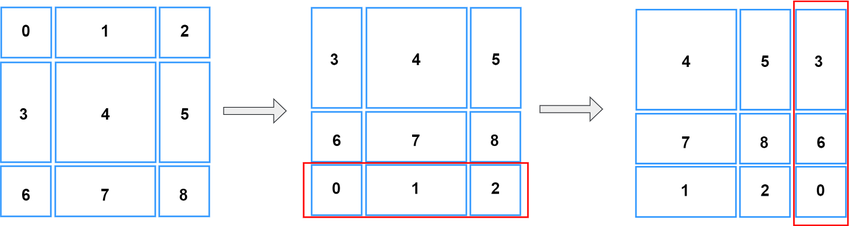
\includegraphics[width=\textwidth]{transformer_images/cycle_shift.png}
		\caption{جا به جایی چرخه ای}
		\label{fig:Cycle Shift in Swin Tranformer}
	\end{minipage}
	\hfill
\end{figure}

در بلوک اول (بدون جابه‌جایی)، پنجره‌ها ثابت‌اند و پیکسل‌های مرزی در هر پنجره ممکن است فرصت کافی برای تبادل اطلاعات با پیکسل‌های مرزیِ پنجرهٔ کناری را نداشته باشند.

در بلوک دوم (جابه‌جاشده)، مرزهای پنجره‌ها تغییر می‌کند و برخی پیکسل‌هایی که قبلاً در پنجره‌های جدا بودند، اکنون در یک پنجرهٔ مشترک‌اند؛ در نتیجه مدل می‌تواند رابطه و همبستگی بین آن‌ها را هم یاد بگیرد.

این جابه‌جایی و قرارگیری مجدد پیکسل‌ها کنار هم در نهایت کمک می‌کند تا مدل بتواند اطلاعات کل تصویر را با هزینهٔ محاسباتی کمتر (نسبت به توجهِ سراسریِ کامل) در اختیار داشته باشد \cite{liu2021swintransformer}.

اگر بخواهیم با مثال توضیح دهیم، فرض کنید در یک تابلوی شطرنجی، خانه‌های کناری همدیگر را «نمی‌بینند» چون در دو بلوک مختلف هستند.
اما اگر کمی تابلوی شطرنجی را به سمت بالا-چپ یا پایین-راست جابه‌جا کنیم،
حالا بخشی از آن خانه‌ها وارد یک بلوک واحد می‌شوند و اطلاعاتشان با هم ترکیب می‌شود.
سپس به‌طور دوره‌ای (\textit{\lr{Cyclic}})، گوشه‌های اضافی را به آن سمت دیگر تابلوی شطرنجی می‌آوریم
تا هیچ چیز از دست نرود.

به این شکل، سِری اول و دوم بلوک‌های مبدل های پنجره متحرک 
تکمیل‌کنندهٔ یکدیگر می‌شوند \cite{liu2021swintransformer}:
\begin{itemize}
	\item \textbf{بلوک اول:} محاسبهٔ توجه در چهارچوب پنجره‌های ثابت.
	\item \textbf{بلوک دوم:} محاسبهٔ  توجه در پنجره‌های جابه‌جاشده که منجر به تعامل بیشتر بین مرزهای مختلف می‌شود.
\end{itemize}


\subsection{پرسپتروون چند لایه}
پس از انجام توجه چند سری پنجره ای جا  به جا شده 
خروجی به یک مسیر \textbf{\lr{MLP}} می‌رود \cite{liu2021swintransformer}. ساختار این \lr{MLP} به‌صورت زیر است:

\begin{equation}
	X' = \mathrm{GELU}(X W_1 + b_1) \; W_2 + b_2,
	\label{eq:gelu_transform}
\end{equation}

که در آن
\[
W_1 \in \mathbb{R}^{C \times (rC)}, 
\quad
W_2 \in \mathbb{R}^{(rC) \times C}
\]
هستند و \(\displaystyle r\) معمولاً ضریب افزایش بعد را نشان می‌دهد (مثلاً ۴). 

تابع فعال‌ساز \lr{GELU} (یا \lr{ReLU} و سایر توابع) نیز در این‌جا قابل استفاده است \cite{hendrycks2016gelu}.

\subsection{ترکیب پچ ها}
در مدل مبدل های پنجره متحرک، ساختار سلسله‌مراتبی به این معناست که ما در چند مرحله (\lr{Stage}) مختلف، نقشهٔ ویژگی را کوچک‌تر می‌کنیم و در عین حال، عمق (تعداد کانال‌های ویژگی) را افزایش می‌دهیم. هدف اصلی از این کار عبارت است از:

\begin{itemize}
	\item \textbf{استخراج ویژگی‌های سطح بالاتر:}
	وقتی نقشهٔ ویژگی کوچک‌تر می‌شود، هر واحد از نقشهٔ ویژگی بیانگر بخش گسترده‌تری از تصویر اصلی است؛ 
	پس مدل به‌تدریج جزئیات محلی را با درک کلی‌تری از تصویر جایگزین می‌کند \cite{he2016deep}.
	
	\item \textbf{کاهش هزینهٔ محاسبات:}
	در مراحل بعدی، چون ابعاد فضایی کمتر می‌شود، مدل راحت‌تر می‌تواند با ویژگی‌های جدید کار کند 
	(چون مثلاً به‌جای \((H \times W)\) پیکسل، تعداد کمتری پیکسل داریم) \cite{liu2021swintransformer}.
\end{itemize}


پس از چندین بلوک پردازشی، نقشهٔ ویژگی، ابعادی به شکل \((\tfrac{H}{P}, \tfrac{W}{P})\) با تعداد کانال \(\displaystyle C\) دارد. 
این یعنی پس از برش‌دادن تصویر به پچ‌ها و گذر از چند لایه، اکنون یک نقشهٔ ویژگی داریم که کوچک‌تر از تصویر اصلی است، 
اما هنوز ممکن است خیلی بزرگ باشد.

در مرحلهٔ بعد (\lr{Stage} بعدی)، می‌خواهیم این نقشه را نصف کنیم 
(یعنی طول و عرض را دو برابر کوچک کنیم) و در عوض عمق کانال را دو برابر کنیم 
(تا ظرفیت مدل در استخراج ویژگی‌های پیچیده‌تر بیشتر شود). برای انجام این کار از فرایندی به نام 
ترکیب پچ‌ها استفاده می‌کنیم.
\cite{liu2021swintransformer}:

\subsubsection{1. انتخاب بلوک‌های \((2 \times 2)\)}
ابتدا نقشهٔ ویژگی را در بُعد مکانی به بلوک‌های \((2 \times 2)\) تقسیم می‌کنیم.  
اگر \(\displaystyle Z_{i,j}\) ویژگیِ مکان \((i, j)\) باشد، 
یک بلوک \((2 \times 2)\) شامل چهار پیکسل است:
\[
Z_{2i, 2j}, \quad Z_{2i, 2j+1}, \quad Z_{2i+1, 2j}, \quad Z_{2i+1, 2j+1}.
\]

\subsubsection{2. ادغام ویژگی‌های چهار پیکسل}
برای هر بلوک \((2 \times 2)\)، این چهار پیکسل را در بُعد کانال به هم می‌چسبانیم.  
اگر هر پیکسل یک بردار از بعد \(\displaystyle C\) باشد، اکنون بعدِ حاصل از کنار هم گذاشتن این چهار پیکسل می‌شود \(\displaystyle 4C\).  
نام این بردار ادغام‌شده را \(\displaystyle Z'\) می‌گذاریم.

\subsubsection{3. لایهٔ خطی برای تغییر بعد}
وقتی چهار بردار \(\displaystyle C\)-بعدی را کنار هم می‌گذاریم، یک بردار \(\displaystyle 4C\)-بعدی شکل می‌گیرد.  
حال با یک لایهٔ خطی، بعدِ \(\displaystyle 4C\) را به بعد جدیدی تبدیل می‌کنیم.  
معمولاً این بعد جدید برابر \(\displaystyle 2C\) در نظر گرفته می‌شود؛ 
یعنی دو برابر بزرگ‌تر از قبل اما نه چهار برابر:
\begin{equation}
	Z' \mapsto Z'' = Z' \, W_{\text{merge}} + b_{\text{merge}},
	\label{eq:merge_transform}
\end{equation}

که بعد ویژگی را از \(\displaystyle 4C\) به \(\displaystyle 2C\) کاهش می‌دهد.

\subsubsection{4. کاهش ابعاد مکانی}
در عین حال، وقتی هر چهار پیکسل \((2 \times 2)\) را ادغام می‌کنیم، 
نقشهٔ ویژگی ما ابعاد فضایی \(\bigl(\tfrac{H}{2P} \times \tfrac{W}{2P}\bigr)\) خواهد داشت 
(چون هر بلوک \((2 \times 2)\) تبدیل به یک بردار می‌شود).

به عبارت دیگر، تعداد نقاط مکانی نصف می‌شود (هم در طول و هم در عرض)، 
اما کانال از \(\displaystyle C\) به \(\displaystyle 2C\) افزایش می‌یابد.

\begin{figure}[h]
	\centering
	\begin{minipage}[b]{1\textwidth}
		\centering
		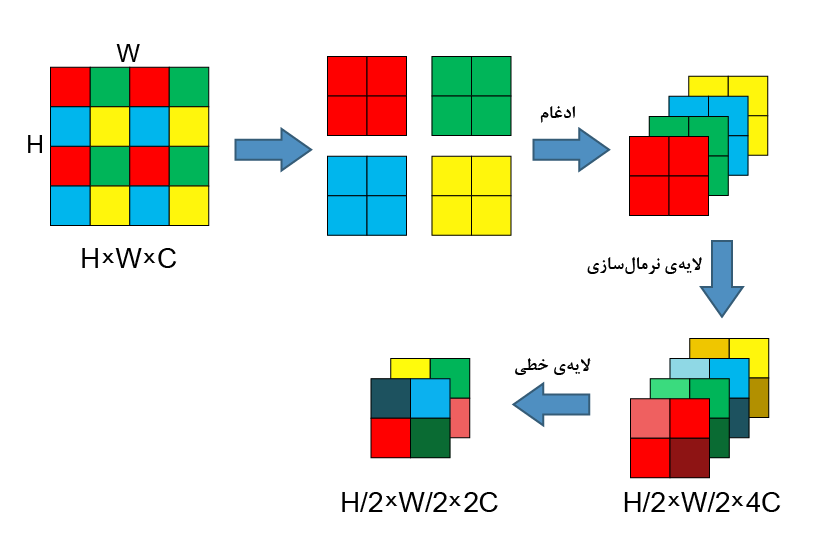
\includegraphics[width=\textwidth]{transformer_images/persian images/b12.png}
		\caption{ادغام پچ ها}
		\label{fig:patch merging in Swin Transformer}
	\end{minipage}
	\hfill
\end{figure}

در شبکه‌های کانولوشنی، مرتبا از لایه‌های ادغام \footnote{\lr{Pooling}} یا کانولوشن با گام \footnote{\lr{Stride-Convolution}} 
برای کوچک‌کردن ابعاد استفاده می‌شود تا اطلاعات سطح بالاتر (مثل ساختار کلی اشیا) راحت‌تر استخراج شود \cite{he2016deep}.  در مبدل پنجره متحرک هم همین ایدهٔ سلسله‌مراتب را به دنیای مبدل ها آورده است \cite{liu2021swintransformer}.  
همچنین اگر ابعاد فضایی را کم نکنیم، هزینهٔ توجه به‌شدت زیاد می‌شود 
(چون باید در هر لایه برای همهٔ پیکسل‌ها توجه محاسبه گردد).

در معماری کلی کبدل های پنجره متحرک، پس از \lr{Stage 1} و عبور از بلوک‌های توجه چند سر پنجره ای و توجه چند سر پنجره ای جابه جا شده، عملیات  ادغام پچ ها انجام می‌شود. سپس در \lr{Stage 2}، ویژگی‌های کوچک‌تری داریم، اما تعداد کانال‌ها افزایش یافته است \cite{liu2021swintransformer}.  
مشابه معماری‌های کانولوشنی، با افزایش عمق \footnote{\lr{Depth}}، ابعاد فضایی کاهش و تعداد کانال‌ها افزایش پیدا می‌کند.

در انتهای \lr{Stage} آخر، خروجی به یک لایهٔ \lr{FC} داده می‌شود تا تعداد کلاس‌ها را پیش‌بینی کند.  
پس از گذر از \lr{Softmax}، احتمال هر کلاس به‌دست می‌آید و مدل در نهایت کلاس نهایی را برمی‌گزیند.







\chapter{روش های پیشنهادی}



\subsection*{استفاده از روش‌های تانسوری در شبکه‌های عصبی چندلایه}

در سال‌های اخیر، استفاده از روش‌های تانسوری به‌عنوان روشی نوین در بهینه‌سازی معماری‌های شبکه‌های عصبی، به‌ویژه در مدل‌هایی که تعداد پارامترهای آن‌ها بسیار زیاد است، مانند شبکه‌های عصبی چندلایه \footnote{\lr{Mlp}}، توجه بسیاری را به خود جلب کرده است \cite{novikov2015tensorizing}. تانسورها تعمیمی از ماتریس‌ها به ابعاد بالاتر هستند و به‌طور طبیعی برای نمایش داده‌های چندبعدی همچون تصاویر، ویدیوها یا سری‌های زمانی چندکاناله مناسب‌اند. بهره‌گیری از ساختار تانسوری در معماری شبکه، این امکان را فراهم می‌سازد که بدون نیاز به فشرده‌سازی اولیه (مانند صاف کردن \footnote{\lr{flatten}} کردن ورودی)، اطلاعات ساختاری میان ابعاد مختلف حفظ شده و مدل بتواند از روابط درون‌تعاملی موجود میان این ابعاد بهره‌برداری نماید \cite{novikov2015tensorizing}.

در معماری سنتی شبکه عصبی چند لایه، نگاشت از ورودی \lr{$\mathbf{x} \in \mathbb{R}^n$} به خروجی \lr{$\mathbf{y} \in \mathbb{R}^m$} به‌وسیله ضرب ماتریسی انجام می‌گیرد:

\[
\mathbf{y} = W\mathbf{x} + \mathbf{b}
\]

که در آن \lr{$W \in \mathbb{R}^{m \times n}$} ماتریس وزن و \lr{$\mathbf{b}$} بردار بایاس است.

\begin{figure}[h]
	\centering
	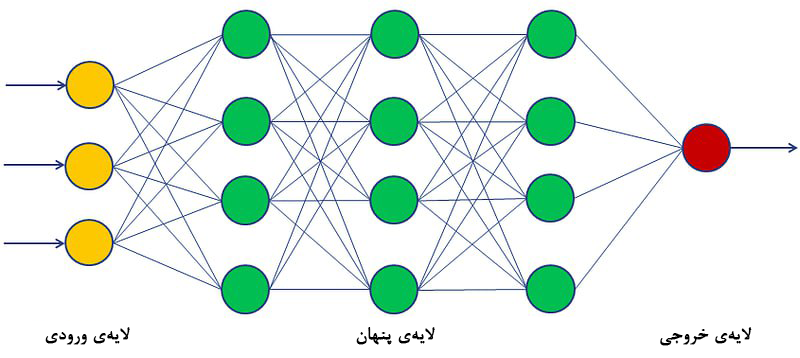
\includegraphics[width=0.8\textwidth]{transformer_images/persian images/b13.png}
	\caption{شبکه عصبی پرسپترون چند لایه}
	\label{fig:Mlp}
\end{figure}

در مقابل، در روش‌های تانسوری، وزن‌ها به‌صورت یک تانسور مرتبه بالاتر مدل‌سازی می‌شوند و نگاشت ورودی به خروجی با استفاده از ضرب‌های چندحالته (ضرب تانسوری در ابعاد مختلف) صورت می‌پذیرد:

\begin{equation}
	\mathbf{y} = \mathcal{W} \times_1 \mathbf{x}_1 \times_2 \mathbf{x}_2 \times_3 \cdots + \mathbf{b}
\end{equation}


در این رابطه، \lr{$\mathcal{W}$} یک تانسور وزن است و عملگر \lr{$\times_n$} نشان‌دهنده ضرب تانسوری در بعد $n$‌ام می‌باشد.

روش‌هایی نظیر \lr{TCL} \footnote{tensor contraction layer} و \lr{TRL} \footnote{Tensor regression layer} به‌عنوان نمونه‌هایی از این رویکرد، با بهره‌گیری از تکنیک‌های تجزیه تانسوری همچون \lr{Tucker} یا تجزیه \lr{CP}، نه تنها باعث کاهش چشمگیر در تعداد پارامترها می‌شوند، بلکه ساختار چندبعدی داده‌ها را نیز حفظ می‌نمایند \cite{kossaifi2017tensorcontraction, kossaifi2020tensorregression}.

\subsection*{مزایای استفاده از روش‌های تانسوری}

استفاده از روش‌های تانسوری در شبکه‌های عصبی چندلایه مزایای متعددی به همراه دارد که برخی از مهم‌ترین آن‌ها عبارت‌اند از:

\begin{itemize}
	\item \textbf{کاهش چشمگیر تعداد پارامترها:} با بهره‌گیری از فشرده‌سازی تانسوری، می‌توان ابعاد تانسور وزن‌ها را به‌گونه‌ای کاهش داد که بدون افت محسوس در عملکرد مدل، مصرف حافظه و پیچیدگی محاسباتی به‌طور قابل توجهی کاهش یابد \cite{lebedev2015cp, kossaifi2020tensorregression}.
	
	\item \textbf{حفظ ساختار داده‌های ورودی:} برخلاف روش‌های سنتی که در آن‌ها داده‌ها پیش از ورود به لایه‌های چگال \footnote{\lr{Dense}} باید مسطح‌سازی \footnote{\lr{Flatten}} شوند، استفاده از ساختار تانسوری این امکان را فراهم می‌کند که ساختار فضایی، زمانی یا کانالی داده‌ها حفظ شده و ارتباط میان ابعاد مختلف ورودی بهتر درک و پردازش شود \cite{kossaifi2020tensorregression}.
\end{itemize}

\subsection*{محدودیت‌ها و چالش‌ها}

با وجود مزایای متعدد، بهره‌گیری از روش‌های تانسوری در معماری‌های شبکه‌های عصبی با چالش‌ها و محدودیت‌هایی نیز همراه است که در ادامه به برخی از مهم‌ترین آن‌ها اشاره می‌شود:

\begin{itemize}
	\item \textbf{پیچیدگی بالاتر در پیاده‌سازی:} پیاده‌سازی لایه‌های مبتنی بر عملیات تانسوری معمولاً به ابزارها و کتابخانه‌های خاصی همچون \lr{Tensorly} یا \lr{Tensor Toolbox} نیاز دارد. این موضوع فرآیند طراحی و توسعه مدل را پیچیده‌تر از استفاده از لایه‌های استاندارد مانند شبکه عصبی چند لایه می‌سازد \cite{kossaifi2017tensorcontraction}.
	
	\item \textbf{بهینه‌سازی دشوارتر:} فرآیند آموزش مدل‌های تانسوری می‌تواند نسبت به مدل‌های معمولی کندتر باشد. الگوریتم‌های مبتنی بر گرادیان ممکن است در فضای پارامتری تانسورها با سطوح خطای غیرهموار یا چندوجهی مواجه شوند که روند همگرایی را دشوار می‌کند \cite{yang2017ttrnn}.
	
	\item \textbf{احتمال کاهش دقت در فشرده‌سازی شدید:} در صورتی‌که میزان فشرده‌سازی تانسورها بیش از حد بالا باشد، مدل ممکن است توانایی لازم برای نمایش روابط غیرخطی و الگوهای پیچیده را از دست داده و در نتیجه، دقت نهایی پیش‌بینی کاهش یابد \cite{kossaifi2020tensorregression}.
\end{itemize}



\subsection{لایه فشرده‌سازی تانسوری}


\lr{Tensor Contraction Layer}

در بسیاری از مدل‌های یادگیری عمیق—به‌ویژه شبکه‌های عصبی کانولوشنی (\lr{convolution})—فعال‌سازی‌های لایه‌های میانی به‌شکل تانسورهایی با مرتبه بالا ظاهر می‌شوند. به‌طور سنتی، برای اعمال لایه‌های کاملاً متصل (\lr{Fully Connected})، این تانسورها ابتدا با عملیات مسطح‌سازی (\lr{flatten}) به بردار تبدیل و سپس به فضای خروجی نگاشت می‌شوند؛ روشی که ساختار چندخطی (\lr{multilinear structure}) داده را از بین برده و به‌تبع، تعداد پارامترها افسارگسیخته افزایش می‌یابد \cite{kossaifi2020tensorregression}.

در پاسخ به این چالش، لایه‌ای با عنوان **­لایهٔ فشرده‌سازی تانسوری** یا به اختصار \lr{TCL} معرفی شده است. این لایه بدون نیاز به مسطح‌سازی، هر مد (mode) از تانسور ورودی را مستقل فشرده‌سازی می‌کند و ساختار چندخطی داده را حفظ می‌نماید \cite{kossaifi2017tensorcontraction,kossaifi2020tensorregression}.



\begin{figure}[h]
	\centering
	\begin{minipage}[b]{0.7\textwidth}
		\centering
		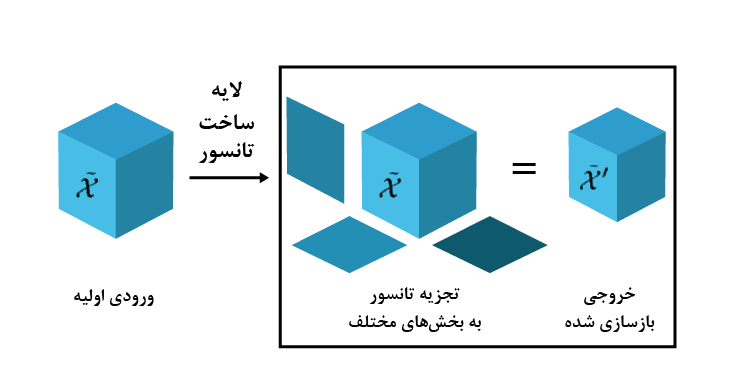
\includegraphics[width=\textwidth]{transformer_images/persian images/b14.png}
		\caption{لایه فشرده ساز تانسوری}
		\label{fig:tensor_contraction_layer}
	\end{minipage}
	\hfill
\end{figure}




\subsubsection*{فرمول‌بندی ریاضی}

فرض کنید تانسور فعال‌سازی ورودی:
\[
\mathcal{X} \in \mathbb{R}^{S \times I_0 \times I_1 \times \cdots \times I_N}
\]
باشد (که \(S\) اندازهٔ دسته‌بندی و \(I_k\)ها ابعاد کانال/فضایی را نشان می‌دهند). هدف لایه TCL، نگاشت:

\begin{equation}
	\mathcal{X}' = \mathcal{X} \times_1 V^{(0)} \times_2 V^{(1)} \cdots \times_{N+1} V^{(N)}
\end{equation}


است، که در آن:
\[
V^{(k)} \in \mathbb{R}^{R_k \times I_k}, \quad \forall k = 0,\dots,N.
\]
با این عملگرهای ضرب چندحالته (\(\times_n\)) تعداد پارامترها به‌شکلی چشمگیر کاهش می‌یابند \cite{kossaifi2017tensorcontraction}.







\subsubsection*{تحلیل تعداد پارامترها}

در TCL، کل پارامترهای قابل آموزش برابر است با:

\begin{equation}
	\text{پارامترهای TCL} = \sum_{k=0}^{N} I_k \cdot R_k
\end{equation}




در حالی‌که در لایه متصل سنتی (پس از مسطح‌سازی):


\begin{equation}
	\text{پارامترهای FC} = \left(\prod_{k=0}^{N} I_k\right) \cdot O
\end{equation}


که \(O\) تعداد نورون‌های خروجی لایه است. نمایش ریاضی بالا به‌وضوح نشان می‌دهد که TCL با جایگزینی ضرب با جمع ساده، به‌صرفه‌سازی قابل‌توجهی در حافظه و محاسبات مدل منجر می‌شود \cite{kossaifi2017tensorcontraction,kossaifi2020tensorregression}.

\subsection{لایهٔ رگرسیون تانسوری (\lr{TRL})}

این لایه، خروجی مدل را مستقیماً از تانسور ورودی تولید می‌کند، بدون مسطح‌سازی؛ به‌طوری‌که ساختار چندبعدی ورودی حفظ و نگاشت خروجی نیز به‌صورت مرتبۀ پایین (low‑rank) مدل شده است \cite{kossaifi2020tensorregression}.

\subsubsection*{فرمول‌بندی ریاضی}

فرض مجدد تانسور:
\[
\mathcal{X} \in \mathbb{R}^{S \times I_0 \times I_1 \times \cdots \times I_N}
\]
و تانسور وزن:
\[
\mathcal{W} \in \mathbb{R}^{I_0 \times I_1 \times \cdots \times I_N \times O}.
\]
نگاشت خروجی:
\begin{equation}
	\mathbf{Y} = \langle \mathcal{X}, \mathcal{W} \rangle_N + \mathbf{b}
\end{equation}

در اینجا عملگر \(\langle \cdot,\cdot \rangle_N\) ضرب داخلی روی \(N\) بعد اول \(\mathcal{W}\) و \(N\) بعد اول \(\mathcal{X}\) را نشان می‌دهد \cite{kossaifi2020tensorregression}.

برای کاهش پارامترها، \(\mathcal{W}\)‌ با کمک تجزیۀ توکر به شکل زیر نوشته می‌شود:

\begin{equation}
	\mathcal{W} = \mathcal{G} \times_0 U^{(0)} \times_1 U^{(1)} \cdots \times_N U^{(N)} \times_{N+1} U^{(N+1)},
\end{equation}


که \(\mathcal{G}\) هستهٔ کم‌مرتبه (core tensor) و \(U^{(k)}\) ماتریس‌های فشرده‌سازی هستند \cite{kossaifi2020tensorregression}.

فرمول نهایی:
\begin{equation}
	\mathbf{Y} = \left\langle 
	\mathcal{X} \times_0 (U^{(0)})^\top \cdots \times_N (U^{(N)})^\top,\ 
	\mathcal{G} \times_{N+1} U^{(N+1)} 
	\right\rangle_N + \mathbf{b}
\end{equation}

که به‌صورت محاسباتی بهینه‌تر عمل می‌کند \cite{kossaifi2020tensorregression}.

\subsubsection*{تحلیل تعداد پارامترها}

در لایه TRL با تجزیۀ \(\text{Tucker}\)، تعداد پارامترها برابر است با:
\begin{equation}
	\text{پارامترهای TRL} = \left(\prod_{k=0}^{N+1} R_k\right) 
	+ \left(\sum_{k=0}^{N} I_k R_k\right) 
	+ R_{N+1} \cdot O,
\end{equation}

که معمولاً بسیار کمتر از تعداد پارامترهای لایه FC است، به‌ویژه هنگامی که \(R_k \ll I_k\) انتخاب شوند \cite{kossaifi2020tensorregression}.


\subsection{چرا در مبدل‌های بینایی از تانسور استفاده می‌کنیم؟}

\subsubsection{۱. \textbf{کاهش تعداد پارامترها و حافظه مصرفی}}

یکی از چالش‌های اصلی در معماری‌های مبتنی بر مبدل‌های بینایی، رشد نمایی تعداد پارامترها در لایه‌های کاملاً متصل، به‌ویژه در بخش‌های انتهایی شبکه است. با جایگزینی این لایه‌ها با ساختارهای تانسوری مانند TCL و TRL، می‌توان از ساختار چندبعدی داده بهره برده و از طریق تجزیه‌های کم‌مرتبه، تعداد پارامترها را به‌صورت چشمگیری کاهش داد \cite{novikov2015tensorizing, kossaifi2017tensorcontraction, kossaifi2020tensorregression}. این جایگزینی نه‌تنها موجب صرفه‌جویی در حافظه می‌شود، بلکه پیچیدگی محاسباتی مدل را نیز کاهش داده و امکان به‌کارگیری آن را در محیط‌های کم‌منبع (مانند دستگاه‌های لبه‌ای و موبایل) فراهم می‌سازد \cite{hamreras2025tensorization}.

\subsubsection{۲. \textbf{افزایش تفسیرپذیری با حفظ ساختار چندخطی داده}}

در حالی‌که عملیات مسطح‌سازی بر روی تانسورهای ورودی، ساختار ارتباطی میان ابعاد داده را از بین می‌برد، استفاده از لایه‌های تانسوری (TCL و TRL) این ساختار چندخطی را حفظ می‌کند. این امر نه‌تنها مدل را برای کار با داده‌های فضایی یا زمانی چندکاناله مطلوب‌تر می‌سازد بلکه \emph{قابلیت تفسیرپذیری پیش‌بینی‌های مدل} را نیز ارتقا می‌دهد. چرا که استحصال ساختارهای فیچر درون تانسوری (مثلاً بعدهای اساسی کابل‌ها) می‌تواند به تشریح بهتر مسیرهای تصمیم‌گیری مدل کمک کند \cite{hamreras2025tensorization}.

\subsubsection{۳. \textbf{کاهش نیاز به داده‌های آموزشی بزرگ}}

مدل‌های بینایی مبتنی بر مبدل، به‌دلیل فقدان سوگیری‌های مکانی ذاتی شبکه‌های کانولوشنی، نیازمند حجم عظیمی از داده برای آموزش مؤثر هستند. با استفاده از لایه‌های تانسوری مانند TCL و TRL که نگاشت‌ها را به‌صورت چندخطی و فشرده مدل‌سازی می‌کنند و ساختار درونی داده را حفظ می‌کنند، می‌توان از ظرفیت مدل به‌صورت بهینه‌تر بهره برد. این ساختار نه‌تنها کمک می‌کند وابستگی‌های میان‌بُعدی بهتر درک شوند بلکه از بیش‌برازش در شرایط داده‌ی محدود جلوگیری می‌کند؛ به‌عنوان مثال، در روش FacT (Factor‑Tuning)، فقط \(0.01\%\) پارامترهای ViT برای تعداد بسیار کمی از نمونه‌های آموزشی آموزش داده می‌شود و با صرفه‌جویی قابل‌توجه در پارامترها، عملکردی مشابه یا بهتر از تنظیم کامل (full‑tuning) ارائه می‌دهد \cite{jie2022fact}.


\subsection{روش تانسوری مبدل پنجره متحرک:}




\subsection{پیاده‌سازی مرحله‌ی  تعبیه پچ
	با استفاده از فشرده‌سازی تانسوری}

در معماری‌های کلاسیک مبتنی بر مبدل های بیانی \footnote{\lr{Vision transformer}}  و همچنین در ساختار مبدل های پنجره ای \footnote{\lr{swin transformer}}، مرحله‌ی اولیه‌ی پردازش تصویر شامل تقسیم تصویر به قطعات کوچک (پچ‌ها) و سپس نگاشت هر پچ به یک بردار نهفته با ابعاد ثابت است. این نگاشت معمولاً با استفاده از یک لایه‌ی خطی \footnote{\lr{linear}} یا پیچشی \footnote{\lr{convolution}} با کرنل و گام برابر با اندازه‌ی پچ انجام می‌شود.

در روش تانسوری به‌جای استفاده از نگاشت برداری ساده، از لایه‌ی فشرده‌سازی تانسوری \footnote{\lr{tensor contruction layer}} برای تبدیل هر پچ به یک تانسور چندبعدی در فضای ویژگی استفاده شده است. این نگاشت تانسوری نه‌تنها باعث حفظ ساختار چندخطی پچ‌ها می‌شود، بلکه با فشرده‌سازی موثر، منجر به کاهش پارامترها می شود.




در ابتدا فرض میکنیم  ورودی مدل تصویری با اندازه‌ی \lr{$(B, C, H, W)$} باشد که در آن:

\begin{itemize}
	\item $B$ اندازه‌ی دسته‌ی آموزشی \footnote{\lr{Batch Size}} است.
	\item $C$ تعداد کانال‌های تصویر (برای مثال ۳ در تصاویر رنگی).
	\item $H \times W$ ابعاد تصویر است.
\end{itemize}

این تصویر با استفاده از پچ‌هایی با اندازه‌ی \lr{$(P \times P)$} به $\frac{H}{P} \times \frac{W}{P}$ قطعه تقسیم می‌شود. سپس با استفاده از عملیات بازآرایی \footnote{\lr{rearrangement}}، ساختار ورودی به شکل زیر تبدیل می‌شود:

\[
\mathcal{X} \in \mathbb{R}^{B \times P_1 \times P_2 \times C_1 \times C_2 \times C_3}
\]

که در آن:

\begin{itemize}
	\item $P_1 = \frac{H}{P}$ و $P_2 = \frac{W}{P}$ به‌ترتیب تعداد پچ‌ها در راستای ارتفاع و عرض تصویر هستند.
	\item $C_1 = P$ و $C_2 = P$ ابعاد مکانی هر پچ‌اند.
	\item $C_3 = C$ تعداد کانال‌های تصویر ورودی است.
\end{itemize}

در این بازنمایی، هر پچ در موقعیت $(i,j)$ به‌صورت یک تانسور سه‌بعدی با ابعاد $C_1 \times C_2 \times C_3$ نمایش داده می‌شود. این ساختار چندبعدی امکان استفاده‌ی مستقیم از عملیات تانسوری بدون نیاز به تخت‌سازی را فراهم می‌سازد.



برای نگاشت هر پچ به فضای نهفته، به جای استفاده از mlp  از یک لایه‌ی فشرده ساز تانسوری  استفاده می‌شود. در واقع سه تا بعد اخر با استفاده از لایه فشرده ساز تنسوری تعبیه میشود.

\[
\mathcal{Z} \in \mathbb{R}^{B \times P_1 \times P_2 \times D_1 \times D_2 \times D_3}
\]

در این ساختار، هر پچ به‌جای تبدیل به یک بردار تخت، به یک تانسور سه‌بعدی در فضای نهفته تبدیل می‌شود. این تانسور ساختار درونی پچ را حفظ کرد می کند. 

\subsubsection*{فرمول‌بندی ریاضی عملیات فشرده‌سازی}

فرض میکنیم  $\mathcal{X}_{patch} \in \mathbb{R}^{C_1 \times C_2 \times C_3}$ نمایانگر یک پچ ورودی باشد. برای فشرده‌سازی این تانسور به فضای نهفته $(D_1, D_2, D_3)$، از سه ماتریس فشرده‌سازی قابل آموزش استفاده می‌شود:

\[
V^{(0)} \in \mathbb{R}^{D_1 \times C_1}, \quad
V^{(1)} \in \mathbb{R}^{D_2 \times C_2}, \quad
V^{(2)} \in \mathbb{R}^{D_3 \times C_3}
\]

عملیات فشرده‌سازی با استفاده از ضرب‌های چندحالته \footnote{\lr{n-mode product}} صورت می‌گیرد:

\begin{equation}
	\mathcal{X}_{emb} = \mathcal{X}_{patch} \times_0 V^{(0)} \times_1 V^{(1)} \times_2 V^{(2)}
\end{equation}


که در آن $\mathcal{X}_{emb} \in \mathbb{R}^{D_1 \times D_2 \times D_3}$ نگاشت نهفته‌ی تانسوری برای آن پچ خواهد بود.

در این مدل ساختار چند بعدی به پج ها داده میشود و همچنین با استفاده از تانسور تعداد پارامتر ها کاهش پیدا میکنند و همچنین ظرفیت مدل نیز افزایش پیدا میکند.




در نتیجه، خروجی نهایی مرحله‌ی تعبیه پچ به‌صورت زیر تعریف می‌شود:

\[
\mathcal{Z} \in \mathbb{R}^{B \times P_1 \times P_2 \times D_1 \times D_2 \times D_3}
\]

که در آن هر پچ به‌صورت یک تانسور کم‌بعد در فضای نهفته نمایش داده شده است.


\subsection{ماژول توجه سلف چندسری مبتنی بر پنجره به‌صورت تانسوری}

همانطور که در فصل قبل بیان شد در ساختار مبدل پنجره ای، جهت کاهش پیچیدگی محاسباتی، از روشی با عنوان  \footnote{\lr{Window-based Multi-Head Self-Attention}}بهره گرفته می‌شود. در این روش، ویژگی‌های مکانی تصویر به پنجره‌های کوچک با اندازه‌ی ثابت (بدون هم‌پوشانی) تقسیم شده و سپس عملیات  خود‌توجهی به‌صورت محلی و درون هر پنجره مستقل انجام می‌گیرد.

در روش تانسوری، به‌جای تولید بردارهای تخت‌شده‌ی $Q$، $K$ و $V$، این بردارها به‌صورت \textbf{تانسورهای چندبعدی} با استفاده از لایه فشرده ساز تانسوری تولید می‌شوند.

\subsubsection*{ ساختار ورودی و تقسیم به پنجره‌ها}

خروجی مرحله تعبیه  به‌صورت تانسوری به صورت زیر است 

\[
\mathcal{X} \in \mathbb{R}^{B \times H \times W \times D_1 \times D_2 \times D_3}
\]



در گام اول، همانند مبدل های پنجره ای به پنجره‌های $w \times w$ تقسیم می‌شوند. و خروجی ما به صورت  زیر خواهد بود.

\[
\mathcal{X}_{win} \in \mathbb{R}^{B \times N_H \times N_W \times w \times w \times D_1 \times D_2 \times D_3}
\]

که در آن $N_H = \frac{H}{w}$ و $N_W = \frac{W}{w}$ به‌ترتیب تعداد پنجره‌ها در راستای ارتفاع و عرض تصویر هستند.

\subsubsection*{2. محاسبه‌ی Q، K و V با استفاده از لایه فشرده ساز تانسوری}

برای هر پنجره‌ی مکانی، سه لایه‌ی فشرده‌سازی تانسوری مستقل (\lr{TCL}) برای استخراج تانسورهای Q، K و V طراحی شده‌اند. فرض می‌شود تانسور ورودی هر پنجره دارای ابعاد:

\[
\mathcal{X}_{patch} \in \mathbb{R}^{w \times w \times D_1 \times D_2 \times D_3}
\]

باشد. با اعمال سه عملیات ضرب n-مد به‌ترتیب در ابعاد تانسوری، نگاشت‌های Q، K و V به‌صورت زیر حاصل می‌شوند:

\begin{equation}
	\mathcal{Q} = \mathcal{X}_{patch} \times_2 V_Q^{(1)} \times_3 V_Q^{(2)} \times_4 V_Q^{(3)}
\end{equation}

\begin{equation}
	\mathcal{K} = \mathcal{X}_{patch} \times_2 V_K^{(1)} \times_3 V_K^{(2)} \times_4 V_K^{(3)}
\end{equation}

\begin{equation}
	\mathcal{V} = \mathcal{X}_{patch} \times_2 V_V^{(1)} \times_3 V_V^{(2)} \times_4 V_V^{(3)}
\end{equation}


که در آن هر $V^{(i)}$ ماتریس فشرده‌سازی با ابعاد $\mathbb{R}^{D_i \times D_i}$ است. بنابراین، خروجی هر لایه به فضای تانسوری مشابه با ورودی بازمی‌گردد:

\[
\mathcal{Q}, \mathcal{K}, \mathcal{V} \in \mathbb{R}^{w \times w \times D_1 \times D_2 \times D_3}
\]

\subsubsection*{3. تقسیم سرهای توجه چندگانه}

برای پیاده‌سازی مکانیزم چندسر\footnote{\lr{multi-head}}، ابعاد تانسوری خروجی به بخش‌های کوچک‌تری تقسیم می‌شود. فرض می‌شود:

\[
D_1 = h_1 \cdot d_1, \quad D_2 = h_2 \cdot d_2, \quad D_3 = h_3 \cdot d_3
\]

که در آن:
\begin{itemize}
	\item $h_1, h_2, h_3$ تعداد سرها در هر بُعد تانسوری،
	\item $d_1, d_2, d_3$ ابعاد نهفته‌ی هر سر در هر بُعد هستند.
\end{itemize}

با استفاده از عملیات بازآرایی، تانسورهای Q، K و V به شکل زیر سازمان‌دهی می‌شوند:

\[
\mathcal{Q}_{head} \in \mathbb{R}^{B \times N_H \times N_W \times w \times w \times h_1 \times h_2 \times h_3 \times d_1 \times d_2 \times d_3}
\]

و ساختار مشابهی برای K و V در نظر گرفته می‌شود.

\subsubsection*{4. محاسبه ماتریس توجه تانسوری}

عملیات ضرب داخلی تعمیم‌یافته بین تانسورهای Q و K برای محاسبه‌ی ماتریس توجه انجام می‌شود. برای هر سر $(a,b,c)$ و برای موقعیت‌های $(i,j)$ و $(k,l)$ در پنجره، مقدار توجه به‌صورت زیر محاسبه می‌شود:

\begin{equation}
	\text{Attention}_{ijkl}^{abc} = \sum_{x=1}^{d_1} \sum_{y=1}^{d_2} \sum_{z=1}^{d_3} 
	Q_{ij}^{abcxyz} \cdot K_{kl}^{abcxyz}
\end{equation}


که نتیجه نهایی یک ماتریس توجه با ابعاد زیر است:

\[
\text{Attention} \in \mathbb{R}^{B \times N_H \times N_W \times h_1 \times h_2 \times h_3 \times w^2 \times w^2}
\]

برای پایدارسازی محاسبات، نرمال‌سازی زیر اعمال می‌شود:

\begin{equation}
	\text{scale} = \frac{1}{\sqrt{d_1 d_2 d_3}}
\end{equation}


و از نسخه علامت‌دار تابع softmax برای اعمال توجه استفاده می‌گردد:

\begin{equation}
	\text{Attention}_{\text{soft}} = \text{sign}(A) \cdot \text{softmax}(|A|)
\end{equation}


\subsubsection*{5. اعمال توجه و بازسازی ویژگی}

پس از محاسبه ماتریس توجه، تانسور خروجی هر پنجره با استفاده از ترکیب توجه و تانسور V محاسبه می‌شود:

\begin{equation}
	\mathcal{Y}_{ij}^{abcxyz} = \sum_{k,l} \text{Attention}_{ijkl}^{abc} \cdot V_{kl}^{abcxyz}
\end{equation}


و پس از انجام توجه برای هر پنجره دوباره باز آرایی میشوند و به حالت اولیه باز میگردند و ابعاد آن به صورت زیر میشود.

\[
\mathcal{Y} \in \mathbb{R}^{B \times H \times W \times D_1 \times D_2 \times D_3}
\]

در این مدل چون سر ها در سه بعد تفسیم میشوند در نتیجه این مدل آزادی خیلی بیشتری دارد.






\subsection{توجه علامت‌دار}

در مکانیزم‌های استاندارد خود توجهی که در مبدل ها مورد استفاده قرار می‌گیرند، ماتریس‌های $Q$, $K$ و $V$ با یکدیگر تعامل دارند تا وزن‌های توجه استخراج شوند. در این فرآیند، بردارهای $Q$  \footnote{\lr{Query}}
 و $K$ 
 
 \footnote{\lr{Key}}
  با استفاده از ضرب داخلی محاسبه می‌شوند و نتیجه برای هر توکن، بیان‌گر میزان اهمیت نسبی سایر توکن‌ها در ارتباط با آن توکن است.

فرمول رایج محاسبه توجه به‌صورت زیر تعریف می‌شود:

\begin{equation}
	\text{Attention}(Q, K, V) = \text{Softmax}\left( \frac{QK^\top}{\sqrt{d_k}} \right) V
\end{equation}

در این ساختار، خروجی $QK^\top$ می‌تواند شامل مقادیر مثبت، منفی یا صفر باشد؛ اما پس از اعمال تابع \lr{Softmax}، تمامی مقادیر به‌صورت نرمال‌سازی‌شده و مثبت خواهند بود. در نتیجه،اطلاعات قطبیت (علامت) که در نتیجه‌ی ضرب داخلی بین بردارهای $Q$ و $K$ وجود داشت، از بین می‌رود. این ویژگی باعث محدود شدن ظرفیت مدل در شناسایی «رابطه منفی یا متضاد» میان توکن‌ها می‌شود.

برای حفظ این اطلاعات قطبیت، د از رویکردی با عنوان  توجه علامت دار استفاده شده است. ایده‌ی اصلی این روش آن است که پس از محاسبه‌ی امتیازهای توجه $A = QK^\top$، عملیات نرمال‌سازی \lr{Softmax} بر قدرمطلق این امتیازها انجام شده و سپس علامت اولیه آن‌ها به نتیجه بازگردانده می‌شود.

فرمول این روش به‌صورت زیر تعریف می‌شود:

\begin{equation}
	\text{Attention}_{\text{sign}} = \text{sign}(A) \cdot \text{Softmax}(|A|)
\end{equation}


که در آن:
\begin{itemize}
	\item $A = QK^\top$ ماتریس امتیازهای اولیه توجه است.
	\item $\text{sign}(A)$ عملیاتی است که علامت هر مقدار را حفظ می‌کند (مقادیر $+1$, $-1$ یا $0$).
	\item $|A|$ قدرمطلق مقادیر است که شدت شباهت را بدون در نظر گرفتن جهت نشان می‌دهد.
\end{itemize}


برای درک بهتر تفاوت میان مکانیزم‌های توجه معمولی و توجه علامت دار یک مثال عددی ساده اما گویای زیر ارائه می‌شود.

فرض کنیم  بردار پرس‌وجو (Q) و دو بردار کلید (K) به‌صورت زیر تعریف شده‌اند:

\[
Q = [1,\ 2,\ -1], \quad
K_1 = [1,\ 0,\ -1], \quad
K_2 = [-1,\ 1,\ 1]
\]

\paragraph{محاسبه امتیاز توجه}

ابتدا شباهت میان Q و هر کلید با استفاده از ضرب داخلی محاسبه می‌شود:

\[
Q \cdot K_1 = (1)(1) + (2)(0) + (-1)(-1) = 1 + 0 + 1 = 2
\]
\[
Q \cdot K_2 = (1)(-1) + (2)(1) + (-1)(1) = -1 + 2 -1 = 0
\]

بنابراین بردار امتیاز توجه به‌صورت زیر حاصل می‌شود:

\[
A = [2,\ 0]
\]

\paragraph{الف) توجه معمولی:}

در توجه معمولی، از تابع softmax مستقیماً روی مقادیر $A$ استفاده می‌شود:

\[
\text{Softmax}(A) =
\left[
\frac{e^2}{e^2 + e^0},\ 
\frac{e^0}{e^2 + e^0}
\right]
\approx [0.88,\ 0.12]
\]

در اینجا، هر دو کلید مقدار وزن مثبت می‌گیرند، حتی اگر امتیاز شباهت دومی برابر با صفر بوده باشد. مدل نمی‌تواند تفاوت میان بی‌اثر بودن و تأثیر منفی یا متضاد را به‌خوبی درک کند.

\paragraph{ب) توجه علامت‌دار:}

در این رویکرد، ابتدا بردار $A$ به دو بخش علامت و قدرمطلق تفکیک می‌شود:

\[
\text{sign}(A) = [1,\ 0], \quad
|A| = [2,\ 0]
\]

سپس تابع softmax فقط روی قدرمطلق‌ها اعمال شده و خروجی زیر حاصل می‌شود:

\[
\text{Softmax}(|A|) = 
\left[
\frac{e^2}{e^2 + e^0},\ 
\frac{e^0}{e^2 + e^0}
\right]
\approx [0.88,\ 0.12]
\]

در نهایت، با ضرب عنصر‌به‌عنصر با علامت‌ها:

\[
\text{Attention}_{\text{sign}} = 
\text{sign}(A) \cdot \text{Softmax}(|A|) = [0.88,\ 0.00]
\]

در این حالت، کلید دوم به‌طور کامل کنار گذاشته شده است، چرا که امتیاز آن صفر بوده و نشانی از تأثیر مثبت یا منفی ندارد.


در توجه معمولی، تمامی مقادیر صفر یا منفی به وزن‌های مثبت نرمال‌سازی می‌شوند. در مقابل، توجه علامت‌دار توانایی تمایز بین ارتباط مثبت، منفی و خنثی را دارد. این قابلیت می‌تواند در مدل‌سازی دقیق‌تر تضادهای معنایی یا شباهت‌های منفی نقش مهمی ایفا کند.


\subsection{توجه مبتنی بر پنجره‌های جابه‌جا‌شده به صورت تانسوری}



توجه پنجره ای دارای یک محدودیت مهم است: پچ‌های واقع در پنجره‌های متفاوت هیچ‌گونه تبادل اطلاعاتی ندارند.
در حالی که ممکن هست این پج ها به هم نزدیک باشند به‌منظور رفع این محدودیت، مبدل های پنجره ای مکانیزم توجه مبتنی بر پنجره جا به جا شده معرفی شده است که در آن پنجره‌ها در برخی لایه‌ها به‌صورت جابه‌جا‌شده تعریف می‌شوند و از ماسک توجه برای جلوگیری از تداخل غیرمجاز استفاده می‌شود.

\subsubsection*{مراحل دقیق مکانیزم }

\begin{enumerate}
	\item \textbf{شیفت چرخشی تانسور ورودی:} خروجی مرحله قبلی  با یک  شیفت چرخه ای 
	\footnote{\lr{cyclic shift}} به اندازه $\lfloor \frac{w}{2} \rfloor$ پیکسل در راستای افقی و عمودی جابه‌جا می‌شود. این جابه‌جایی باعث می‌شود که پچ‌هایی که پیش‌تر در پنجره‌های جداگانه بودند، اکنون در یک پنجره جدید قرار گیرند.
	
	به این شیفت روی بعد اول و دوم تانسور که مکان پج را مشخص میکرد صورت میگیرد.
	
	\item \textbf{اعمال پنجره‌بندی جدید:} تانسور جابه‌جا‌شده به پنجره‌های بدون هم‌پوشانی جدید با اندازه $w \times w$ تقسیم می‌شود. پنجره‌های جدید از موقعیت‌های مختلف تصویر تشکیل شده‌اند.
	
	\item \textbf{اعمال خودتوجهی به‌صورت محلی با ماسک:} از آنجا که پنجره‌ها پس از شیفت ممکن است شامل توکن‌هایی از مکان‌های نامرتبط باشند، نیاز است که \textbf{توجه به‌صورت مفید  انجام شود. یک ماسک دودویی روی ماتریس توجه اعمال می‌شود که فقط اجازه توجه به توکن‌هایی را می‌دهد که واقعاً در یک پنجره معتبر قرار دارند.}
	
\end{enumerate}



خودتوجهی پنجره جابه جا شده باعث ارتباط میان پج های نزدیکی میشود که در خودتوجهی پنجره ای در یک پنجره قرار نداشته اند. 



\subsection{ادغام پچ‌ها به‌صورت تانسوری}

در مدل‌های سلسله‌مراتبی بینایی مانند پس از هر مرحله از استخراج ویژگی، لازم است ابعاد مکانی تصویر کاهش یابد تا ویژگی‌ها در سطوح بالاتر به‌صورت فشرده‌تر و معنایی‌تر نمایش داده شوند. این فرایند با عنوان ادغام پچ‌ها \footnote{\lr{Patch Merging}} شناخته می‌شود. در نسخه‌ی اصلی این مدل، ادغام پچ‌ها با استفاده از ترکیب ۴ پچ مجاور (به‌صورت یک پنجره‌ی $2 \times 2$) و سپس اعمال یک لایه‌ی خطی پس از مسطح‌سازی انجام می‌شود. این کار باعث نصف شدن ابعاد مکانی و افزایش ابعاد ویژگی می‌شود.

در این پژوهش، رویکرد متفاوتی برای ادغام پچ‌ها ارائه شده است که مبتنی بر نگاشت تانسوری است. به‌جای انجام \footnote{\lr{flatten}} بر روی پچ‌ها، از ساختار چندبعدی پچ‌ها استفاده شده و با کمک یک لایه‌ی فشرده‌سازی تانسوری، ادغام پچ‌ها بدون از بین رفتن ساختار چندخطی آن‌ها انجام می‌شود.

\subsubsection*{ساختار ورودی}

مانند  خروجی مرحله قبلی شبکه دارای ساختار تانسوری زیر باشد:

\[
\mathcal{X} \in \mathbb{R}^{B \times H \times W \times R_1 \times R_2 \times C}
\]

که در آن:

\begin{itemize}
	\item $B$ اندازه دسته آموزشی،  
	\item $H \times W$ ابعاد مکانی پچ‌ها،  
	\item $(R_1, R_2, C)$ ابعاد فضای نهفته‌ی هر پچ به‌صورت تانسوری.
\end{itemize}

هدف این مرحله، کاهش ابعاد مکانی به $\left( \frac{H}{2}, \frac{W}{2} \right)$ و در عین حال، افزایش غنای بازنمایی ویژگی‌ها است.

\subsubsection*{ادغام پچ‌های مجاور}

برای کاهش ابعاد مکانی، ابتدا هر چهار پچ مجاور در پنجره‌ای $2 \times 2$ انتخاب می‌شوند. این چهار پچ به‌صورت زیر دسته‌بندی می‌شوند:

\begin{itemize}
	\item پچ بالا-چپ،
	\item پچ بالا-راست،
	\item پچ پایین-چپ،
	\item پچ پایین-راست.
\end{itemize}

در مرحله بعد، این چهار پچ با یکدیگر ترکیب می‌شوند، به این صورت که هرکدام به‌صورت مستقل نگه داشته شده و در امتداد بعد کانالی $(C)$ به یکدیگر متصل می‌شوند. در نتیجه، در هر موقعیت مکانی جدید، تانسوری با ابعاد $(R_1, R_2, 4C)$ خواهیم داشت. در سطح کلان، خروجی میان‌مرحله‌ای به‌صورت زیر خواهد بود:

\[
\mathcal{X}_{\text{merged}} \in \mathbb{R}^{B \times \frac{H}{2} \times \frac{W}{2} \times R_1 \times R_2 \times 4C}
\]

\subsubsection*{فشرده‌سازی ویژگی‌های ادغام‌شده}

پس از ادغام کانالی، لازم است ابعاد ویژگی‌ها به صورت کنترل‌شده کاهش یابد تا بتوان آن را به شکل ورودی ماژول‌های بعدی تطبیق داد. برای این منظور، از یک لایه‌ی فشرده‌سازی تانسوری استفاده می‌شود که به‌صورت مستقیم بر روی ابعاد نهفته $(R_1, R_2, 4C)$ عمل می‌کند. برخلاف لایه‌های خطی کلاسیک، در اینجا عملیات فشرده‌سازی در چندین بعد به‌صورت همزمان و با حفظ ساختار چندخطی انجام می‌شود.

خروجی حاصل، تانسوری با ساختار:

\[
\mathcal{Y} \in \mathbb{R}^{B \times \frac{H}{2} \times \frac{W}{2} \times R_1' \times R_2' \times C'}
\]

که در آن $(R_1', R_2', C')$ ابعاد جدید ویژگی‌ها هستند و با توجه به محدودیت طراحی، باید رابطه زیر میان ابعاد قدیم و جدید برقرار باشد:



\begin{equation}
	2 \cdot R_1' \cdot R_2' \cdot C' = 4 \cdot R_1 \cdot R_2 \cdot C
\end{equation}

این رابطه تضمین می‌کند که ادغام از نظر اطلاعاتی قابل‌پشتیبانی و از نظر مدل‌سازی متوازن باقی می‌ماند.



\subsection{مرحله‌ی طبقه‌بندی نهایی با استفاده از رگرسیون تانسوری}

پس از عبور تصویر ورودی از مراحل سلسله‌مراتبی مختلف شامل تعبیه پچ، ماژول‌های خودتوجهی تانسوری، و لایه‌های ادغام و فشرده‌سازی، خروجی نهایی آخرین مرحله به‌صورت یک تانسور چندبعدی در فضای نهفته حاصل می‌شود. این تانسور حاوی بازنمایی غنی از ویژگی‌های سطح بالا و ساختار درونی تصویر است که برای تصمیم‌گیری نهایی مورد استفاده قرار می‌گیرد.

\subsubsection*{میانگین‌گیری تانسوری در ابعاد مکانی}

فرض میکنیم خروجی مرحله‌ی نهایی دارای ساختار تانسوری زیر باشد:

\[
\mathcal{X} \in \mathbb{R}^{B \times H \times W \times D_1 \times D_2 \times D_3}
\]


برای استخراج یک بازنمایی کلی از کل تصویر، میانگین‌گیری در دو بُعد مکانی $(H, W)$ انجام می‌شود. 
در واقع همانند مبدل پنجره ای متحرک از مکان های پچ ها میانگین گیری گرفته میشود 
این عملیات باعث فشرده‌سازی اطلاعات مکانی و حفظ ساختار تانسوری در فضای ویژگی می‌شود.

\begin{equation}
	\bar{\mathcal{X}} = \frac{1}{H \cdot W} \sum_{i=1}^{H} \sum_{j=1}^{W} \mathcal{X}_{[:, i, j, :, :, :]} 
	\in \mathbb{R}^{B \times D_1 \times D_2 \times D_3}
\end{equation}


این عملیات نوعی تجمیع جهانی در ابعاد فضایی محسوب می‌شود که مشابه با میانگین‌گیری سراسری \footnote{\lr{global average pooling}}  در شبکه‌های پیچشی عمل می‌کند، با این تفاوت که ساختار تانسوری ویژگی‌ها را حفظ می‌نماید.

\subsubsection*{طبقه‌بندی با استفاده از لایه رگرسیون تانسوری}

برای نگاشت خروجی $\bar{\mathcal{X}}$ به برچسب نهایی، از یک لایه رگرسیون تانسوری (TRL) استفاده شده است. این لایه با بهره‌گیری از ضرب داخلی تعمیم‌یافته میان تانسور ورودی و تانسور وزن، نگاشتی خطی از فضای تانسوری به فضای خروجی اعمال می‌کند:

\begin{equation}
	\mathbf{Y} = \langle \bar{\mathcal{X}}, \mathcal{W} \rangle_3 + \mathbf{b}
\end{equation}

که در آن
\begin{itemize}
	\item $\bar{\mathcal{X}} \in \mathbb{R}^{B \times D_1 \times D_2 \times D_3}$ بازنمایی فشرده‌ی ورودی،
	\item $\mathcal{W} \in \mathbb{R}^{D_1 \times D_2 \times D_3 \times C}$ تانسور وزن‌های رگرسیون،
	\item $\langle \cdot, \cdot \rangle_3$ ضرب داخلی تعمیم‌یافته در سه بعد آخر $\bar{\mathcal{X}}$ و سه بعد اول $\mathcal{W}$ است،
	\item $\mathbf{b} \in \mathbb{R}^{C}$ بردار بایاس،
	\item $C$ تعداد کلاس‌های خروجی است.
\end{itemize}










\chapter{نتایج و تحلیل‌ها}

\section{ارزیابی بر روی مجموعه‌داده \lr{CIFAR-10}}

به منظور ارزیابی عملکرد مدل پیشنهادی، دو پیکربندی مجزا مورد مقایسه قرار گرفتند:  
\begin{enumerate}
	\item مدل مبنا: \lr{Tiny Swin Transformer} به عنوان معماری اصلی بدون اعمال تغییرات.
	\item مدل پیشنهادی: \lr{Tensorized Swin Transformer} که در آن لایه‌های \lr{Patch Embedding}، \lr{W-MSA} و \lr{Patch Merging} به کمک تکنیک فشرده‌سازی تانسوری بازطراحی شده‌اند.
\end{enumerate}

\subsection{خلاصه نتایج کمی}

جدول \ref{tab:cifar10_summary_tensor} نتایج کمی این دو مدل را در شاخص‌های دقت \lr{Top-1} و \lr{Top-5} برای داده‌های آموزش و آزمون نشان می‌دهد.  
در این جدول ترتیب ستون‌ها به‌گونه‌ای تنظیم شده است که مقایسه میان عملکرد آموزشی و آزمونی به‌صورت هم‌زمان و از راست به چپ قابل مشاهده باشد.

\begin{table}[ht]
	\centering
	\caption{مقایسه عملکرد مدل اصلی و مدل پیشنهادی بر روی مجموعه‌داده \lr{CIFAR-10} بر حسب دقت‌های \lr{Top-1} و \lr{Top-5}.}
	\label{tab:cifar10_summary_tensor}
	\begin{tabular}{ccccccl}
		\hline
		\multicolumn{2}{c}{داده آزمون} & \multicolumn{2}{c}{داده آموزش} & \multirow{2}{*}{\#پارامترها} & \multirow{2}{*}{مدل} \\
		\cline{1-4}
		Top-5 & Top-1 & Top-5 & Top-1 &  &  \\
		\hline
		\lr{96.45\%} & \lr{80.92\%} & \lr{99.97\%} & \lr{97.48\%} & \lr{27,528,690} & \lr{Tiny Swin} \\
		\lr{99.21\%} & \lr{81.80\%} & \lr{98.97\%} & \lr{80.30\%} & \lr{1,368,626} & \lr{Tensorized Swin} \\
		\hline
	\end{tabular}
\end{table}

\subsection{تحلیل نتایج}

مطابق داده‌های جدول \ref{tab:cifar10_summary_tensor}، مدل پیشنهادی با وجود کاهش چشم‌گیر تعداد پارامترها (از حدود \lr{27.5M} به حدود \lr{1.37M}، معادل کاهش \lr{95\%})، توانسته است دقت آزمون را حفظ یا حتی اندکی بهبود بخشد.  
در شاخص \lr{Top-1}، دقت مدل اصلی در داده آزمون برابر \lr{80.92\%} بوده که در مدل تانسوری به \lr{81.80\%} رسیده است.  
همچنین در شاخص \lr{Top-5}، بهبود محسوس‌تری مشاهده می‌شود؛ به‌طوری که مقدار دقت از \lr{96.45\%} به \lr{99.21\%} افزایش یافته است.  

از سوی دیگر، بررسی شکاف آموزش–آزمون نشان می‌دهد که مدل اصلی با اختلاف \lr{16.56} واحد درصد بین دقت آموزشی (\lr{97.48\%}) و آزمونی (\lr{80.92\%}) دچار بیش‌برازش (\lr{Overfitting}) بوده است.  
در حالی که مدل تانسوری نه تنها چنین شکافی ندارد، بلکه دقت آزمونی آن اندکی از دقت آموزشی بیشتر است (اختلاف \lr{-1.5} واحد درصد).  
این امر بیانگر وجود نوعی منظم‌سازی ذاتی (\lr{Implicit Regularization}) ناشی از فشرده‌سازی تانسوری و اعمال قیود کم‌مرتبه (\lr{Low-Rank Constraints}) است.  

بهبود محسوس در \lr{Top-5} نیز حاکی از آن است که مدل پیشنهادی فضای ویژگی غنی‌تری ایجاد کرده که امکان پوشش کلاس‌های صحیح در میان پنج پیش‌بینی برتر را افزایش داده و در نتیجه اطمینان کلی تصمیم‌گیری مدل را ارتقاء داده است.

\subsection{نمایش روند آموزش}

برای درک بهتر فرایند همگرایی، روند تغییرات دقت \lr{Top-1} در طول آموزش برای هر دو مدل در شکل‌های \ref{fig:cifar10_swin_original} و \ref{fig:cifar10_tensorized} نمایش داده شده است.  
این نمودارها نشان می‌دهند که مدل اصلی به سرعت به دقت بالایی در داده آموزشی می‌رسد ولی در داده آزمون افت می‌کند، در حالی که مدل تانسوری با روندی یکنواخت‌تر و پایدارتر به دقت نهایی می‌رسد.

\begin{figure}[ht]
	\centering
	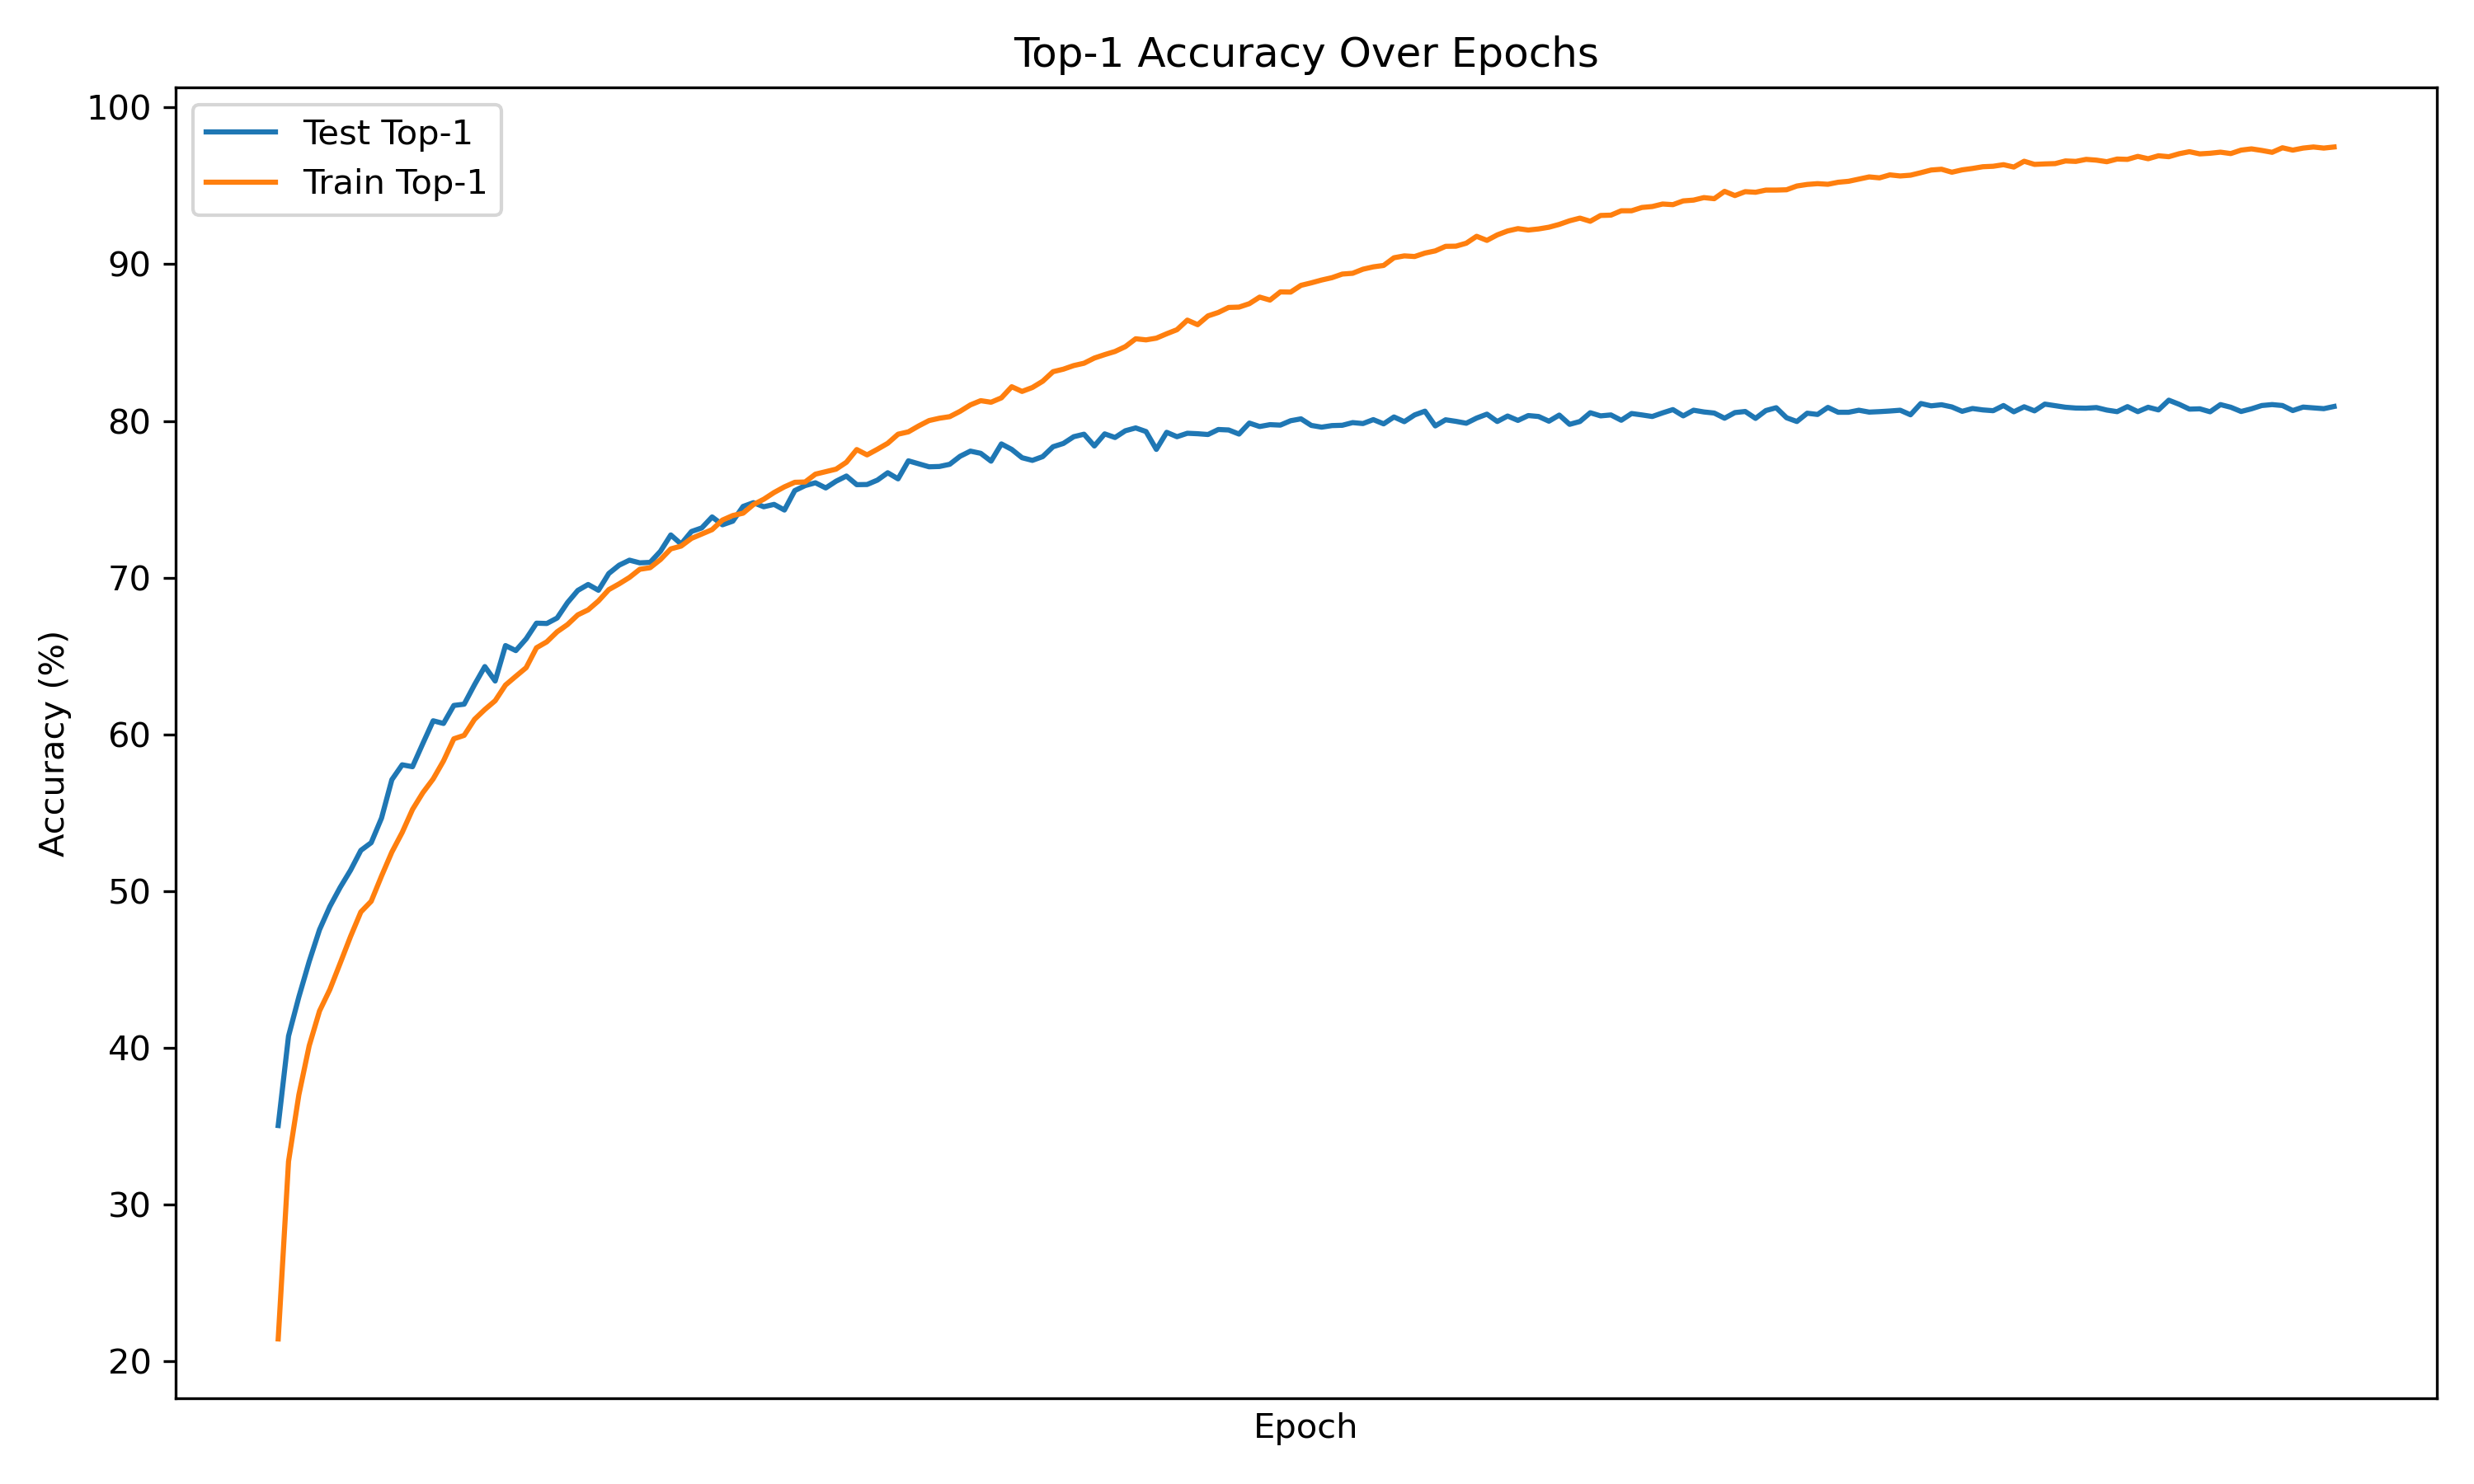
\includegraphics[width=0.85\textwidth]{transformer_images/results/cifar10_swin_original.png}
	\caption{روند تغییرات دقت \lr{Top-1} مدل اصلی \lr{Swin-Tiny} بر روی مجموعه‌داده \lr{CIFAR-10}.}
	\label{fig:cifar10_swin_original}
\end{figure}

\begin{figure}[ht]
	\centering
	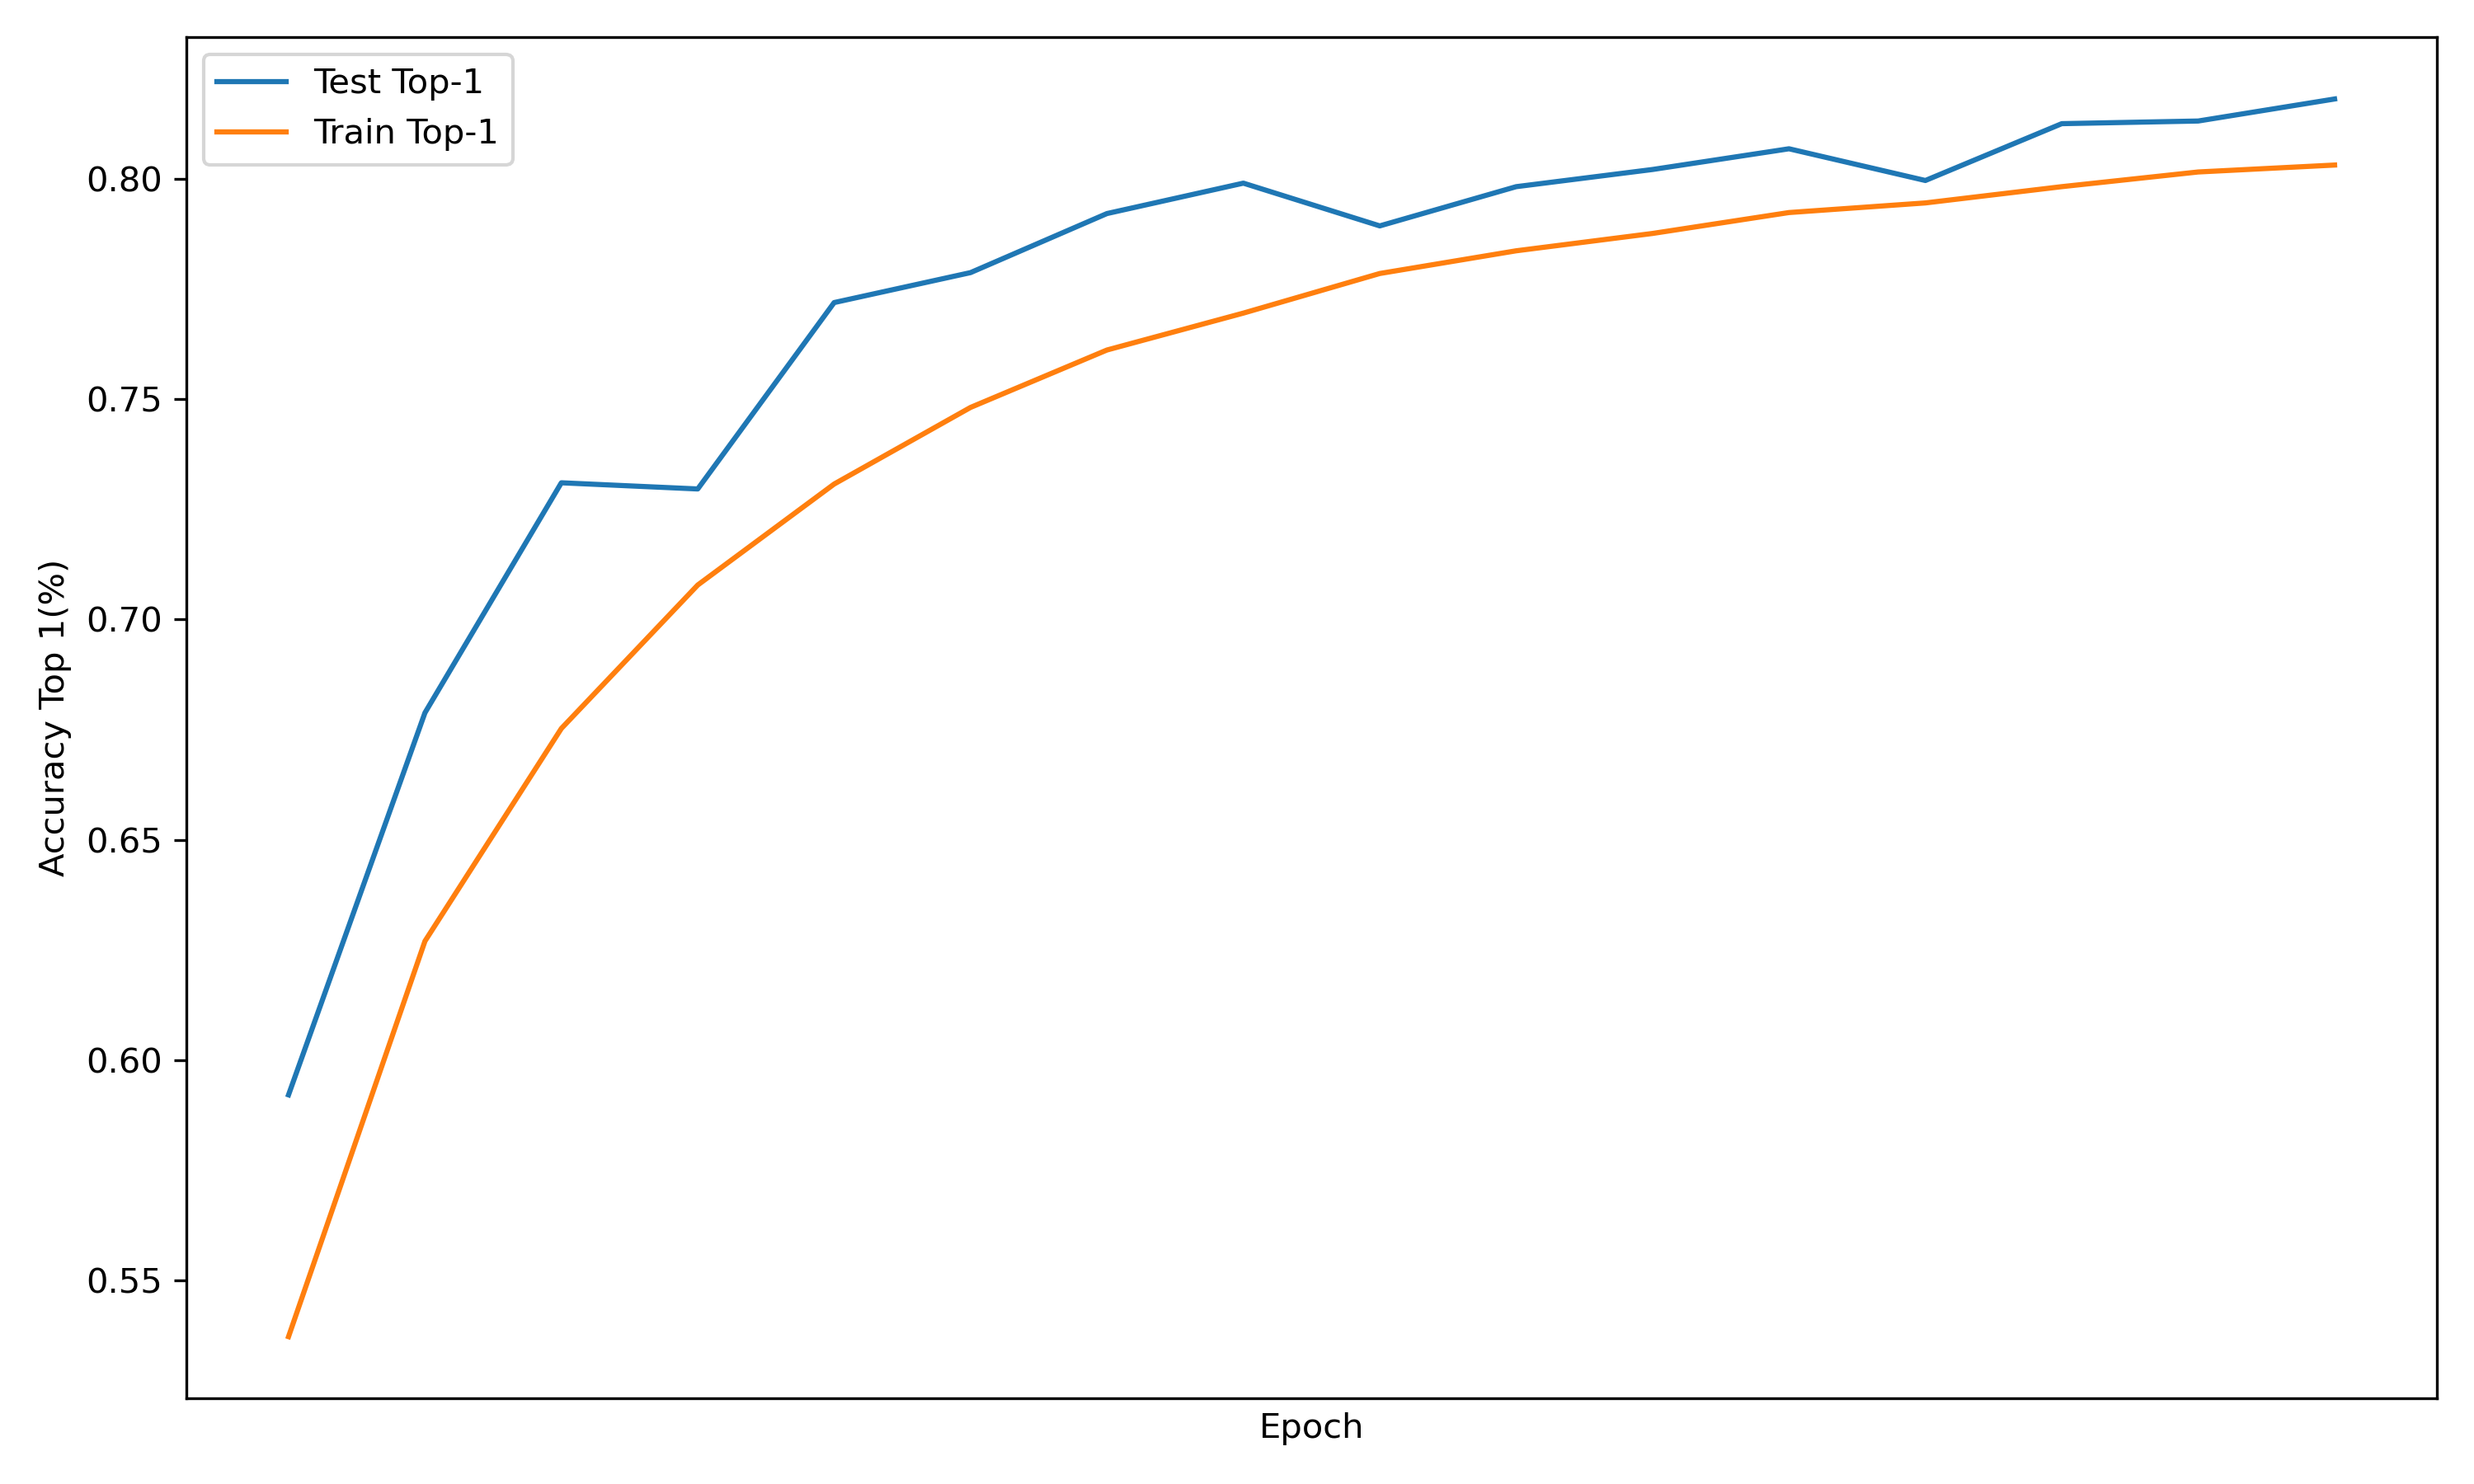
\includegraphics[width=0.85\textwidth]{transformer_images/results/cifar10_tensorized.png}
	\caption{روند تغییرات دقت \lr{Top-1} مدل پیشنهادی \lr{Tensorized Swin} بر روی مجموعه‌داده \lr{CIFAR-10}.}
	\label{fig:cifar10_tensorized}
\end{figure}

\subsection{جمع‌بندی}

به‌طور کلی، نتایج به‌دست‌آمده نشان می‌دهد که استفاده از ساختار تانسوری در بخش‌های کلیدی مدل، علاوه بر کاهش چشم‌گیر پیچیدگی محاسباتی و نیاز حافظه، باعث بهبود تعمیم‌پذیری و کاهش بیش‌برازش نیز می‌شود.  
این امر اهمیت به‌کارگیری روش‌های فشرده‌سازی ساختاریافته را در طراحی مدل‌های کارا برای کاربردهای کم‌منبع تأیید می‌کند.







\section{نتایج بر روی دیتاست \lr{MNIST}}

برای ارزیابی عملکرد مدل پیشنهادی بر روی داده‌های ساده‌تر و با ابعاد کوچک‌تر، آزمایش‌ها بر روی دیتاست \lr{MNIST} نیز انجام شده است. در این ارزیابی دو پیکربندی زیر مقایسه شده‌اند:
\begin{enumerate}
	\item \textbf{مدل اصلی} (\lr{Tiny Swin Transformer})
	\item \textbf{مدل پیشنهادی تانسوری} (\lr{Tensorized Swin Transformer})
\end{enumerate}

\subsection{خلاصه‌ی نتایج کمی}

\begin{table}[ht]
	\centering
	\caption{مقایسه‌ی عملکرد مدل اصلی و مدل تانسوری بر روی \lr{MNIST} (فقط Top-1 و Top-5).}
	\label{tab:mnist_summary_tensor}
	\begin{tabular}{ccccccl} % ستون‌ها به صورت معکوس برای نمایش پایان‌نامه‌ای
		\hline
		\multicolumn{2}{c}{تست} & \multicolumn{2}{c}{آموزش} & \multirow{2}{*}{\#پارامترها} & \multirow{2}{*}{مدل} \\
		\cline{1-4}
		Top-5 & Top-1 & Top-5 & Top-1 &  &  \\
		\hline
		\lr{99.9\%} & \lr{97.0\%} & \lr{99.9\%} & \lr{95.8\%} & \lr{27,528,690} & \lr{Tiny Swin} \\
		\lr{100\%} & \lr{98.9\%} & \lr{99.9\%} & \lr{97.3\%} & \lr{1,368,626} & \lr{Tensorized Swin} \\
		\hline
	\end{tabular}
\end{table}

\subsection{نمایش روند آموزش}

شکل‌های \ref{fig:mnist_swin_original} و \ref{fig:mnist_tensorized} روند تغییرات دقت \lr{Top-1} را برای مدل اصلی و مدل تانسوری بر روی مجموعه‌داده‌ی \lr{MNIST} نشان می‌دهند. هر دو مدل به سرعت به دقت بسیار بالا رسیده‌اند، اما مدل تانسوری با وجود تعداد پارامترهای بسیار کمتر، دقت نهایی بالاتری در داده‌های آزمون کسب کرده است.

\begin{figure}[ht]
	\centering
	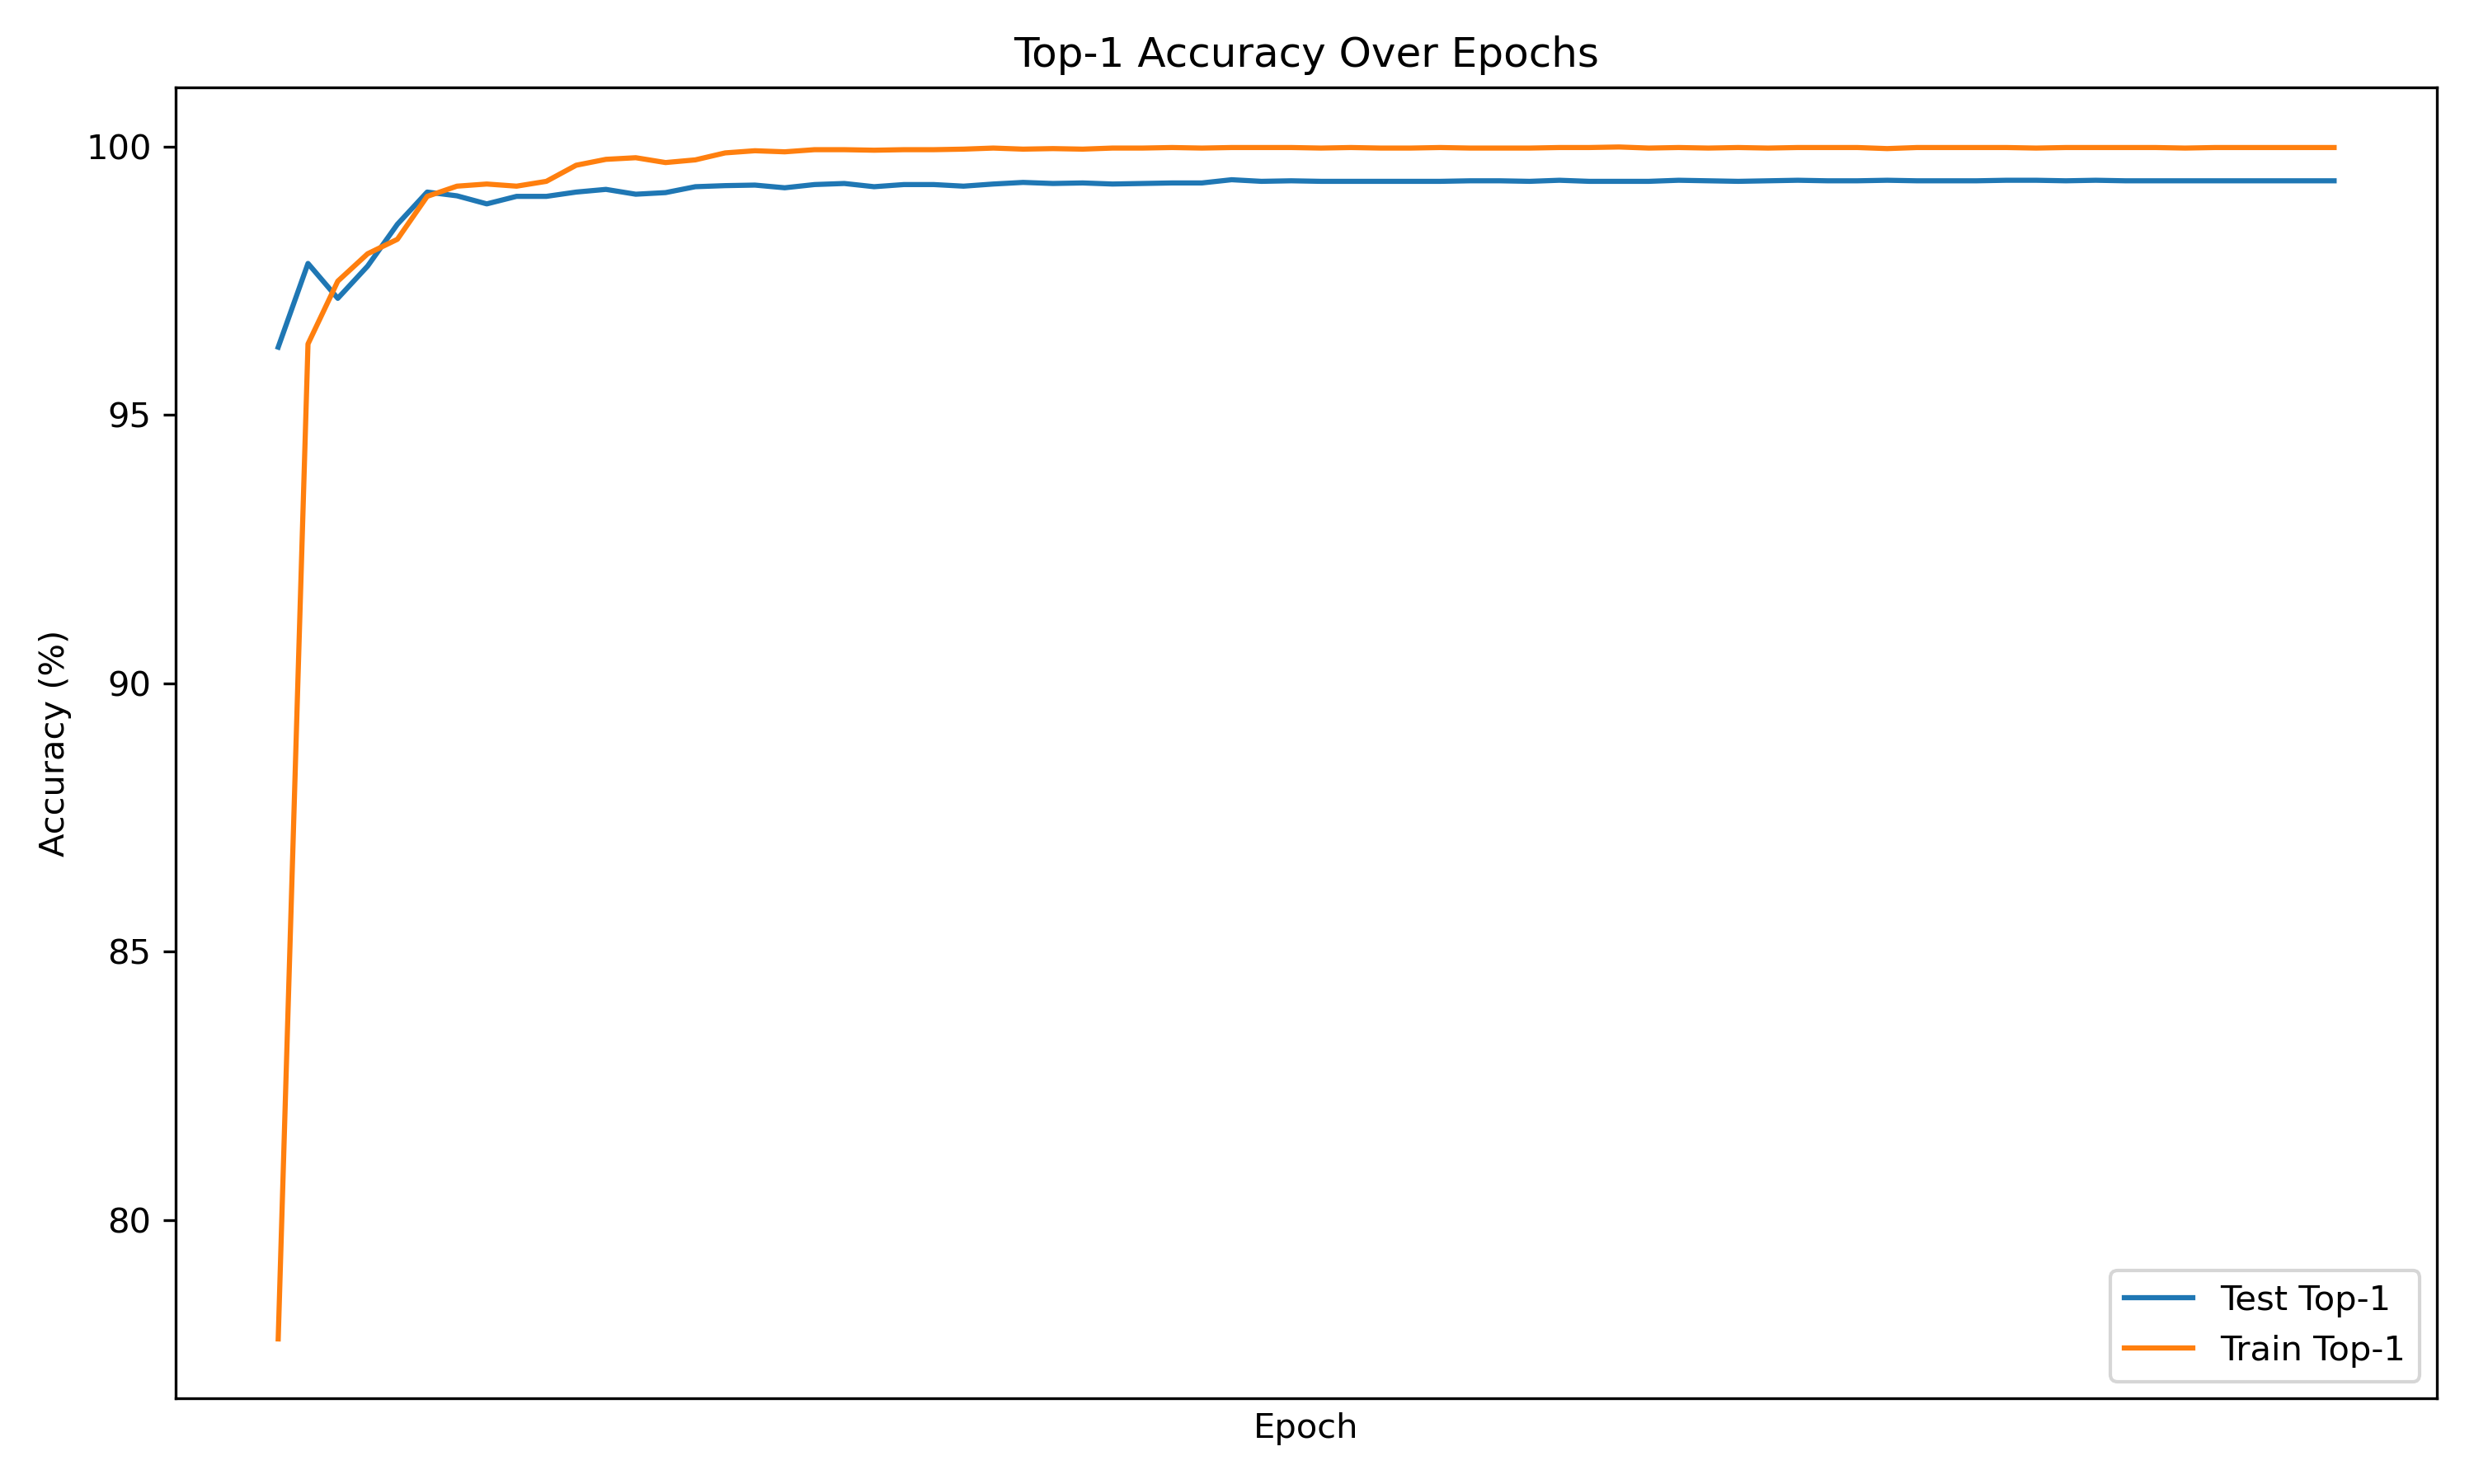
\includegraphics[width=0.85\textwidth]{transformer_images/results/mnist_original.png}
	\caption{روند دقت \lr{Top-1} مدل اصلی \lr{Swin-Tiny} بر روی \lr{MNIST}.}
	\label{fig:mnist_swin_original}
\end{figure}

\begin{figure}[ht]
	\centering
	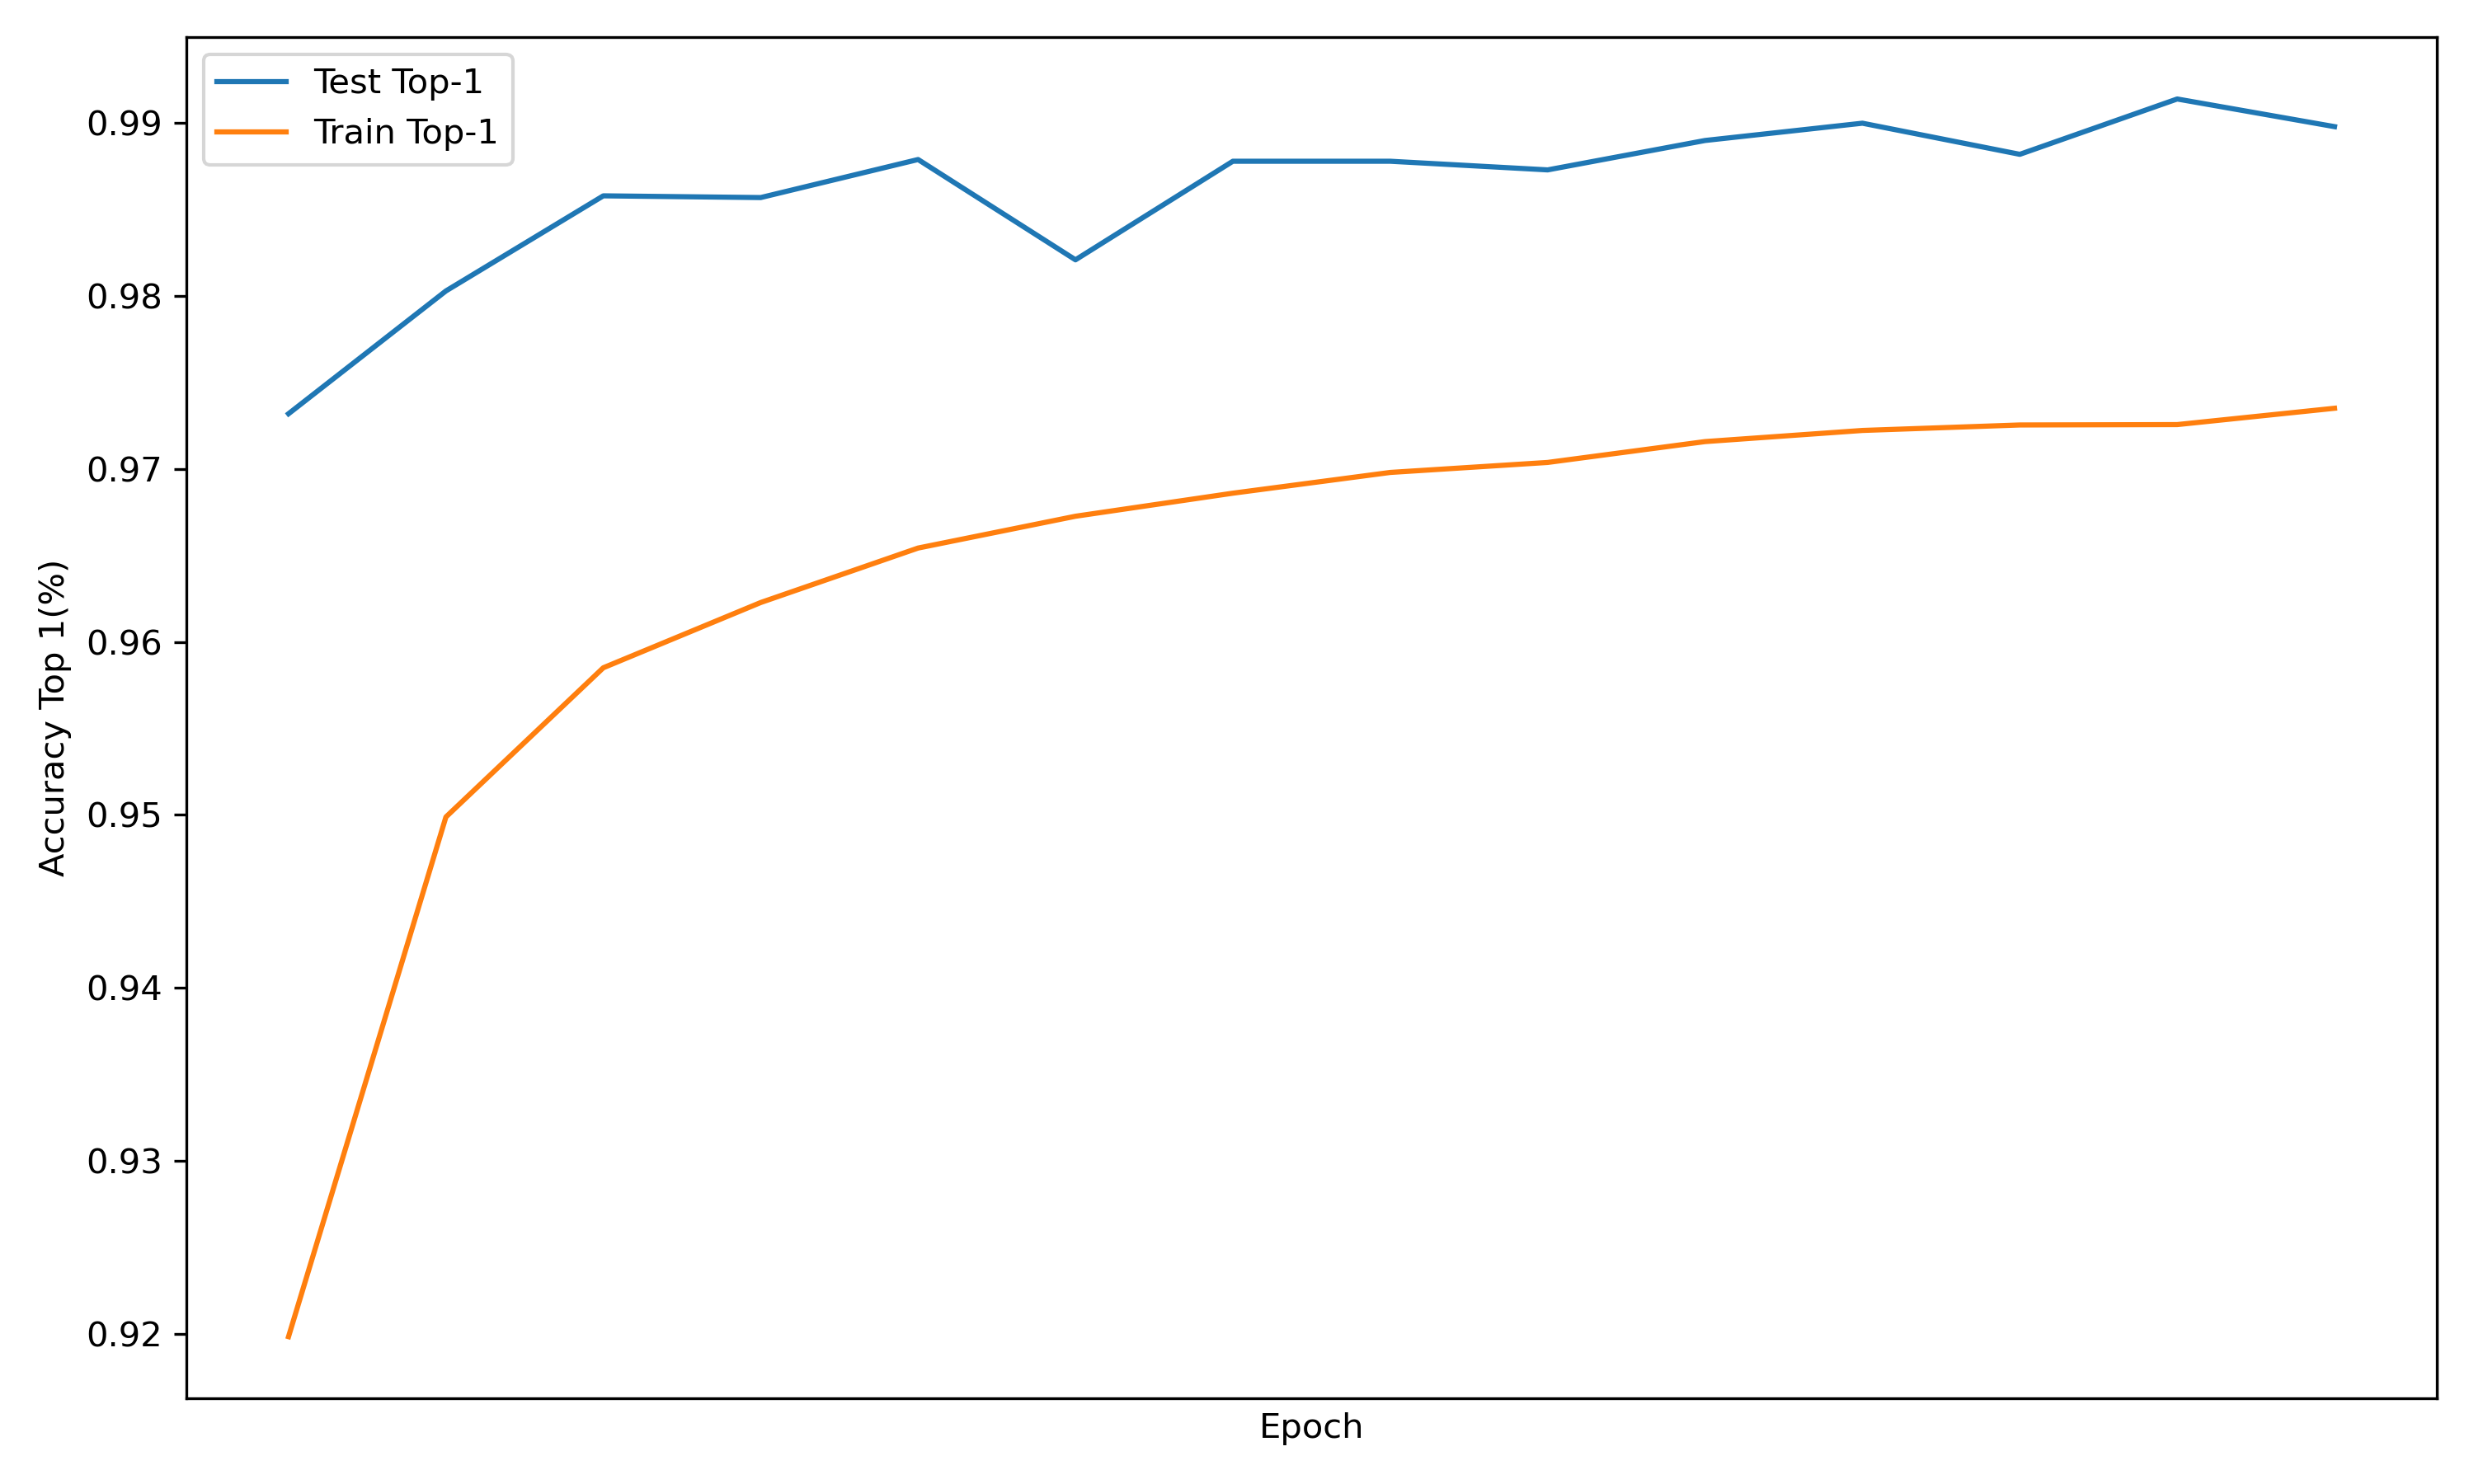
\includegraphics[width=0.85\textwidth]{transformer_images/results/mnist_tensorized.png}
	\caption{روند دقت \lr{Top-1} مدل تانسوری پیشنهادی بر روی \lr{MNIST}.}
	\label{fig:mnist_tensorized}
\end{figure}

\subsection{تحلیل و بحث}

نتایج جدول \ref{tab:mnist_summary_tensor} نشان‌دهنده‌ی نکات مهم زیر است:
\begin{itemize}
	\item \textbf{کاهش چشمگیر پارامترها:} مدل تانسوری فقط \lr{1,368,626} پارامتر دارد در حالی‌که مدل اصلی \lr{27,528,690} پارامتر دارد؛ یعنی کاهش حدوداً \textbf{\lr{20.1} برابر} (نزدیک به \textbf{\lr{95\%}} کاهش در تعداد پارامترها).
	\item \textbf{بهبود دقت آزمون:} دقت \lr{Top-1} آزمون از \textbf{\lr{97.0\%}} در مدل اصلی به \textbf{\lr{98.9\%}} در مدل تانسوری رسیده است (بهبود مطلق \textbf{\lr{+1.9}} واحد درصد). همچنین دقت \lr{Top-5} از \textbf{\lr{99.9\%}} به \textbf{\lr{100\%}} افزایش یافته است.
	\item \textbf{کاهش شکاف آموزش–آزمون:} در مدل اصلی شکاف بین آموزش و آزمون برای \lr{Top-1} برابر \textbf{\lr{1.2}} واحد درصد است (95.8 در برابر 97.0). در مدل تانسوری این شکاف به \textbf{\lr{-1.6}} واحد درصد رسیده است که نشان‌دهنده‌ی عملکرد پایدارتر و تعمیم‌پذیری بهتر است.
	\item \textbf{پایداری در داده‌های ساده‌تر:} با وجود سادگی مجموعه‌داده‌ی \lr{MNIST}، مدل تانسوری همچنان توانسته است دقت را نسبت به مدل اصلی بهبود دهد، که بیانگر قدرت فشرده‌سازی تانسوری در حفظ یا حتی افزایش دقت در کنار کاهش منابع محاسباتی است.
\end{itemize}

\paragraph{جمع‌بندی.} بر اساس نتایج به‌دست‌آمده، مدل تانسوری نه‌تنها حجم مدل را به‌شدت کاهش داده است، بلکه توانسته در یک مجموعه‌داده‌ی ساده مانند \lr{MNIST}، دقت آزمون را نسبت به مدل اصلی افزایش دهد. این نتایج مؤید این است که فشرده‌سازی تانسوری می‌تواند حتی در شرایطی که داده‌ها ساده هستند نیز به‌عنوان یک رویکرد بهینه و کارا مورد استفاده قرار گیرد.







\section{نتایج بر روی دیتاست \lr{Tiny ImageNet}}

برای بررسی عملکرد مدل در یک سناریوی چالش‌برانگیزتر، آزمایش‌هایی بر روی دیتاست \lr{Tiny ImageNet} انجام شد. در این بخش، علاوه بر مدل اصلی \lr{Tiny Swin Transformer}، مدل پیشنهادی تانسوری نیز با دو بهینه‌ساز متفاوت (\lr{Adam} و \lr{AdamW}) ارزیابی شده است.

\subsection{خلاصه نتایج کمی}

\begin{table}[ht]
	\centering
	\caption{مقایسه‌ی عملکرد مدل‌ها بر روی \lr{Tiny ImageNet}.}
	\label{tab:tinyimagenet_summary}
	\begin{tabular}{ccccccc}
		\hline
		\multicolumn{2}{c}{آزمون} & \multicolumn{2}{c}{آموزش} & \#پارامتر & مدل & بهینه‌ساز \\
		\cline{1-4}
		Top-5 & Top-1 & Top-5 & Top-1 &  &  &  \\
		\hline
		\lr{85.42\%} & \lr{64.14\%} & \lr{59.03\%} & \lr{42.26\%} & \lr{27,528,690} & \lr{Tiny Swin} & -- \\
		\lr{54.17\%} & \lr{30.85\%} & \lr{98.50\%} & \lr{83.89\%} & \lr{1,368,626} & \lr{Tensorized Swin} & \lr{Adam} \\
		\lr{62.07\%} & \lr{35.90\%} & \lr{80.90\%} & \lr{55.30\%} & \lr{1,368,626} & \lr{Tensorized Swin} & \lr{AdamW} \\
		\hline
	\end{tabular}
\end{table}

\subsection{نمایش روند آموزش}

شکل \ref{fig:tiny_original_top1} روند تغییر دقت \lr{Top-1} را برای مدل اصلی \lr{Tiny Swin} نشان می‌دهد.  
همچنین، شکل‌های \ref{fig:tiny_tensor_adam} و \ref{fig:tiny_tensor_adamw} مربوط به مدل تانسوری با بهینه‌سازهای \lr{Adam} و \lr{AdamW} هستند.

\begin{figure}[ht]
	\centering
	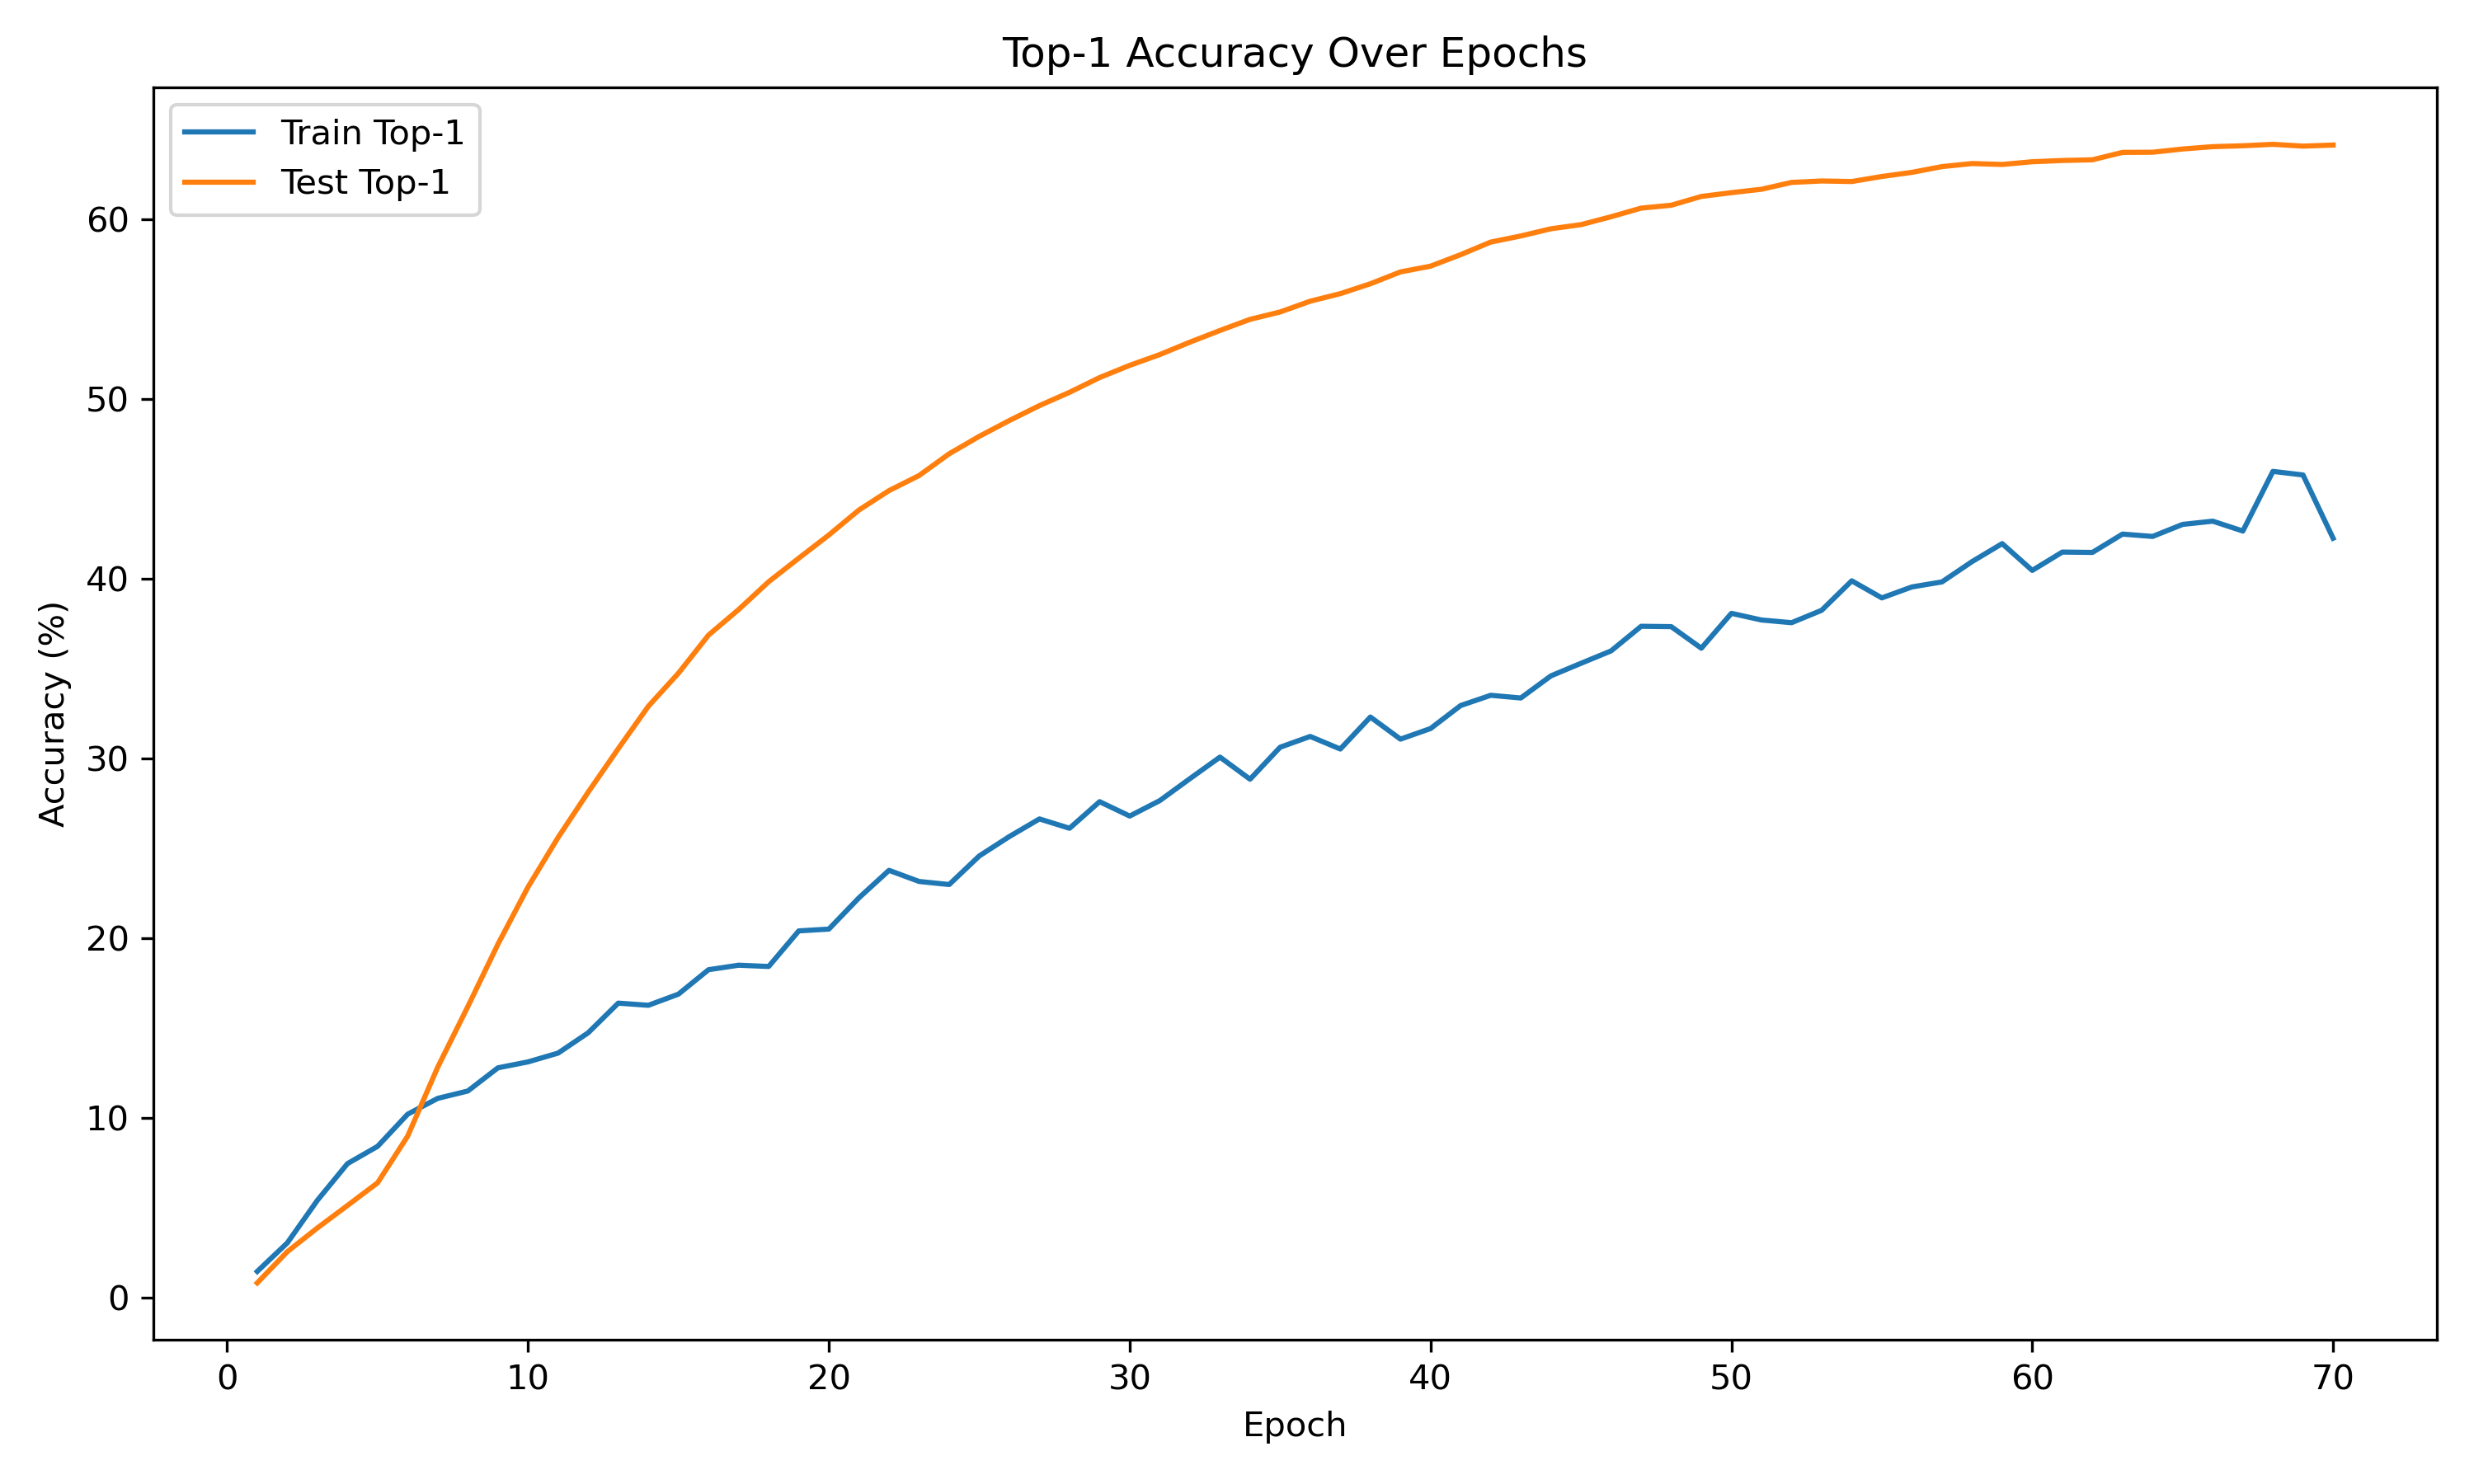
\includegraphics[width=0.85\textwidth]{transformer_images/results/tiny_image_net_original.png}
	\caption{روند دقت \lr{Top-1} مدل اصلی \lr{Tiny Swin} بر روی \lr{Tiny ImageNet}.}
	\label{fig:tiny_original_top1}
\end{figure}

\begin{figure}[ht]
	\centering
	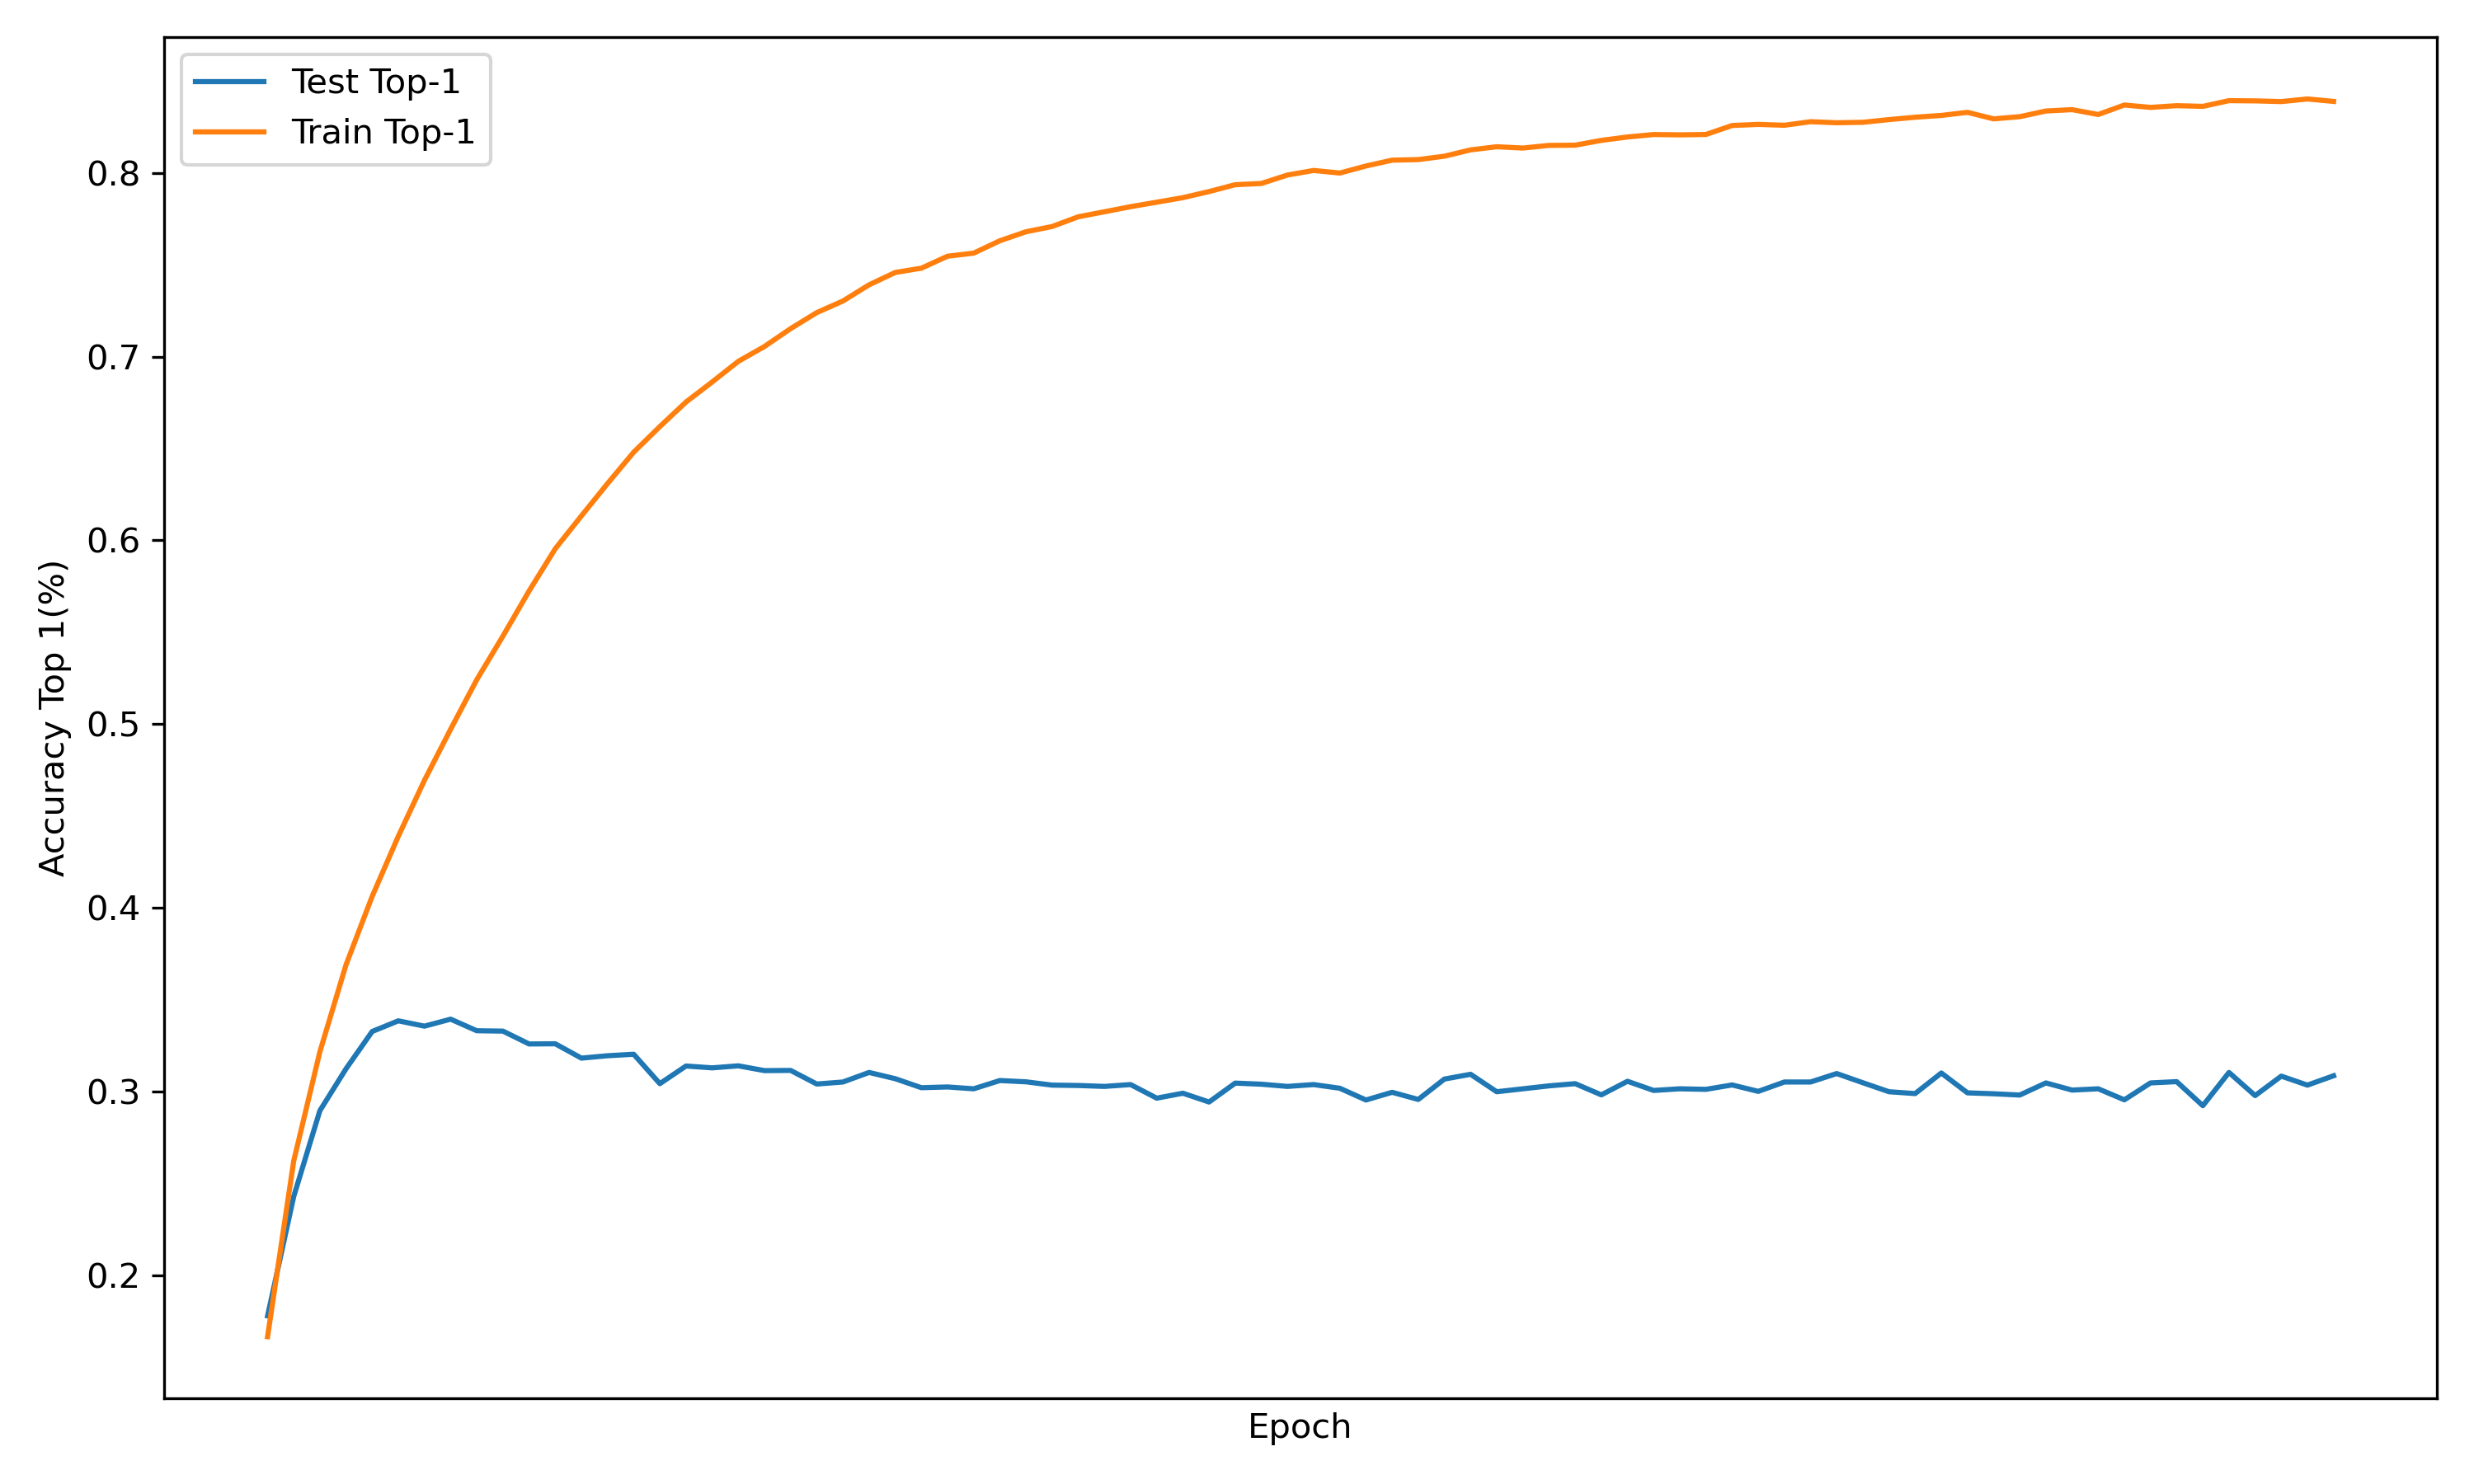
\includegraphics[width=0.85\textwidth]{transformer_images/results/tiny_image_net_tensorized_2.png}
	\caption{روند دقت \lr{Top-1} مدل تانسوری با بهینه‌ساز \lr{Adam} بر روی \lr{Tiny ImageNet}.}
	\label{fig:tiny_tensor_adam}
\end{figure}

\begin{figure}[ht]
	\centering
	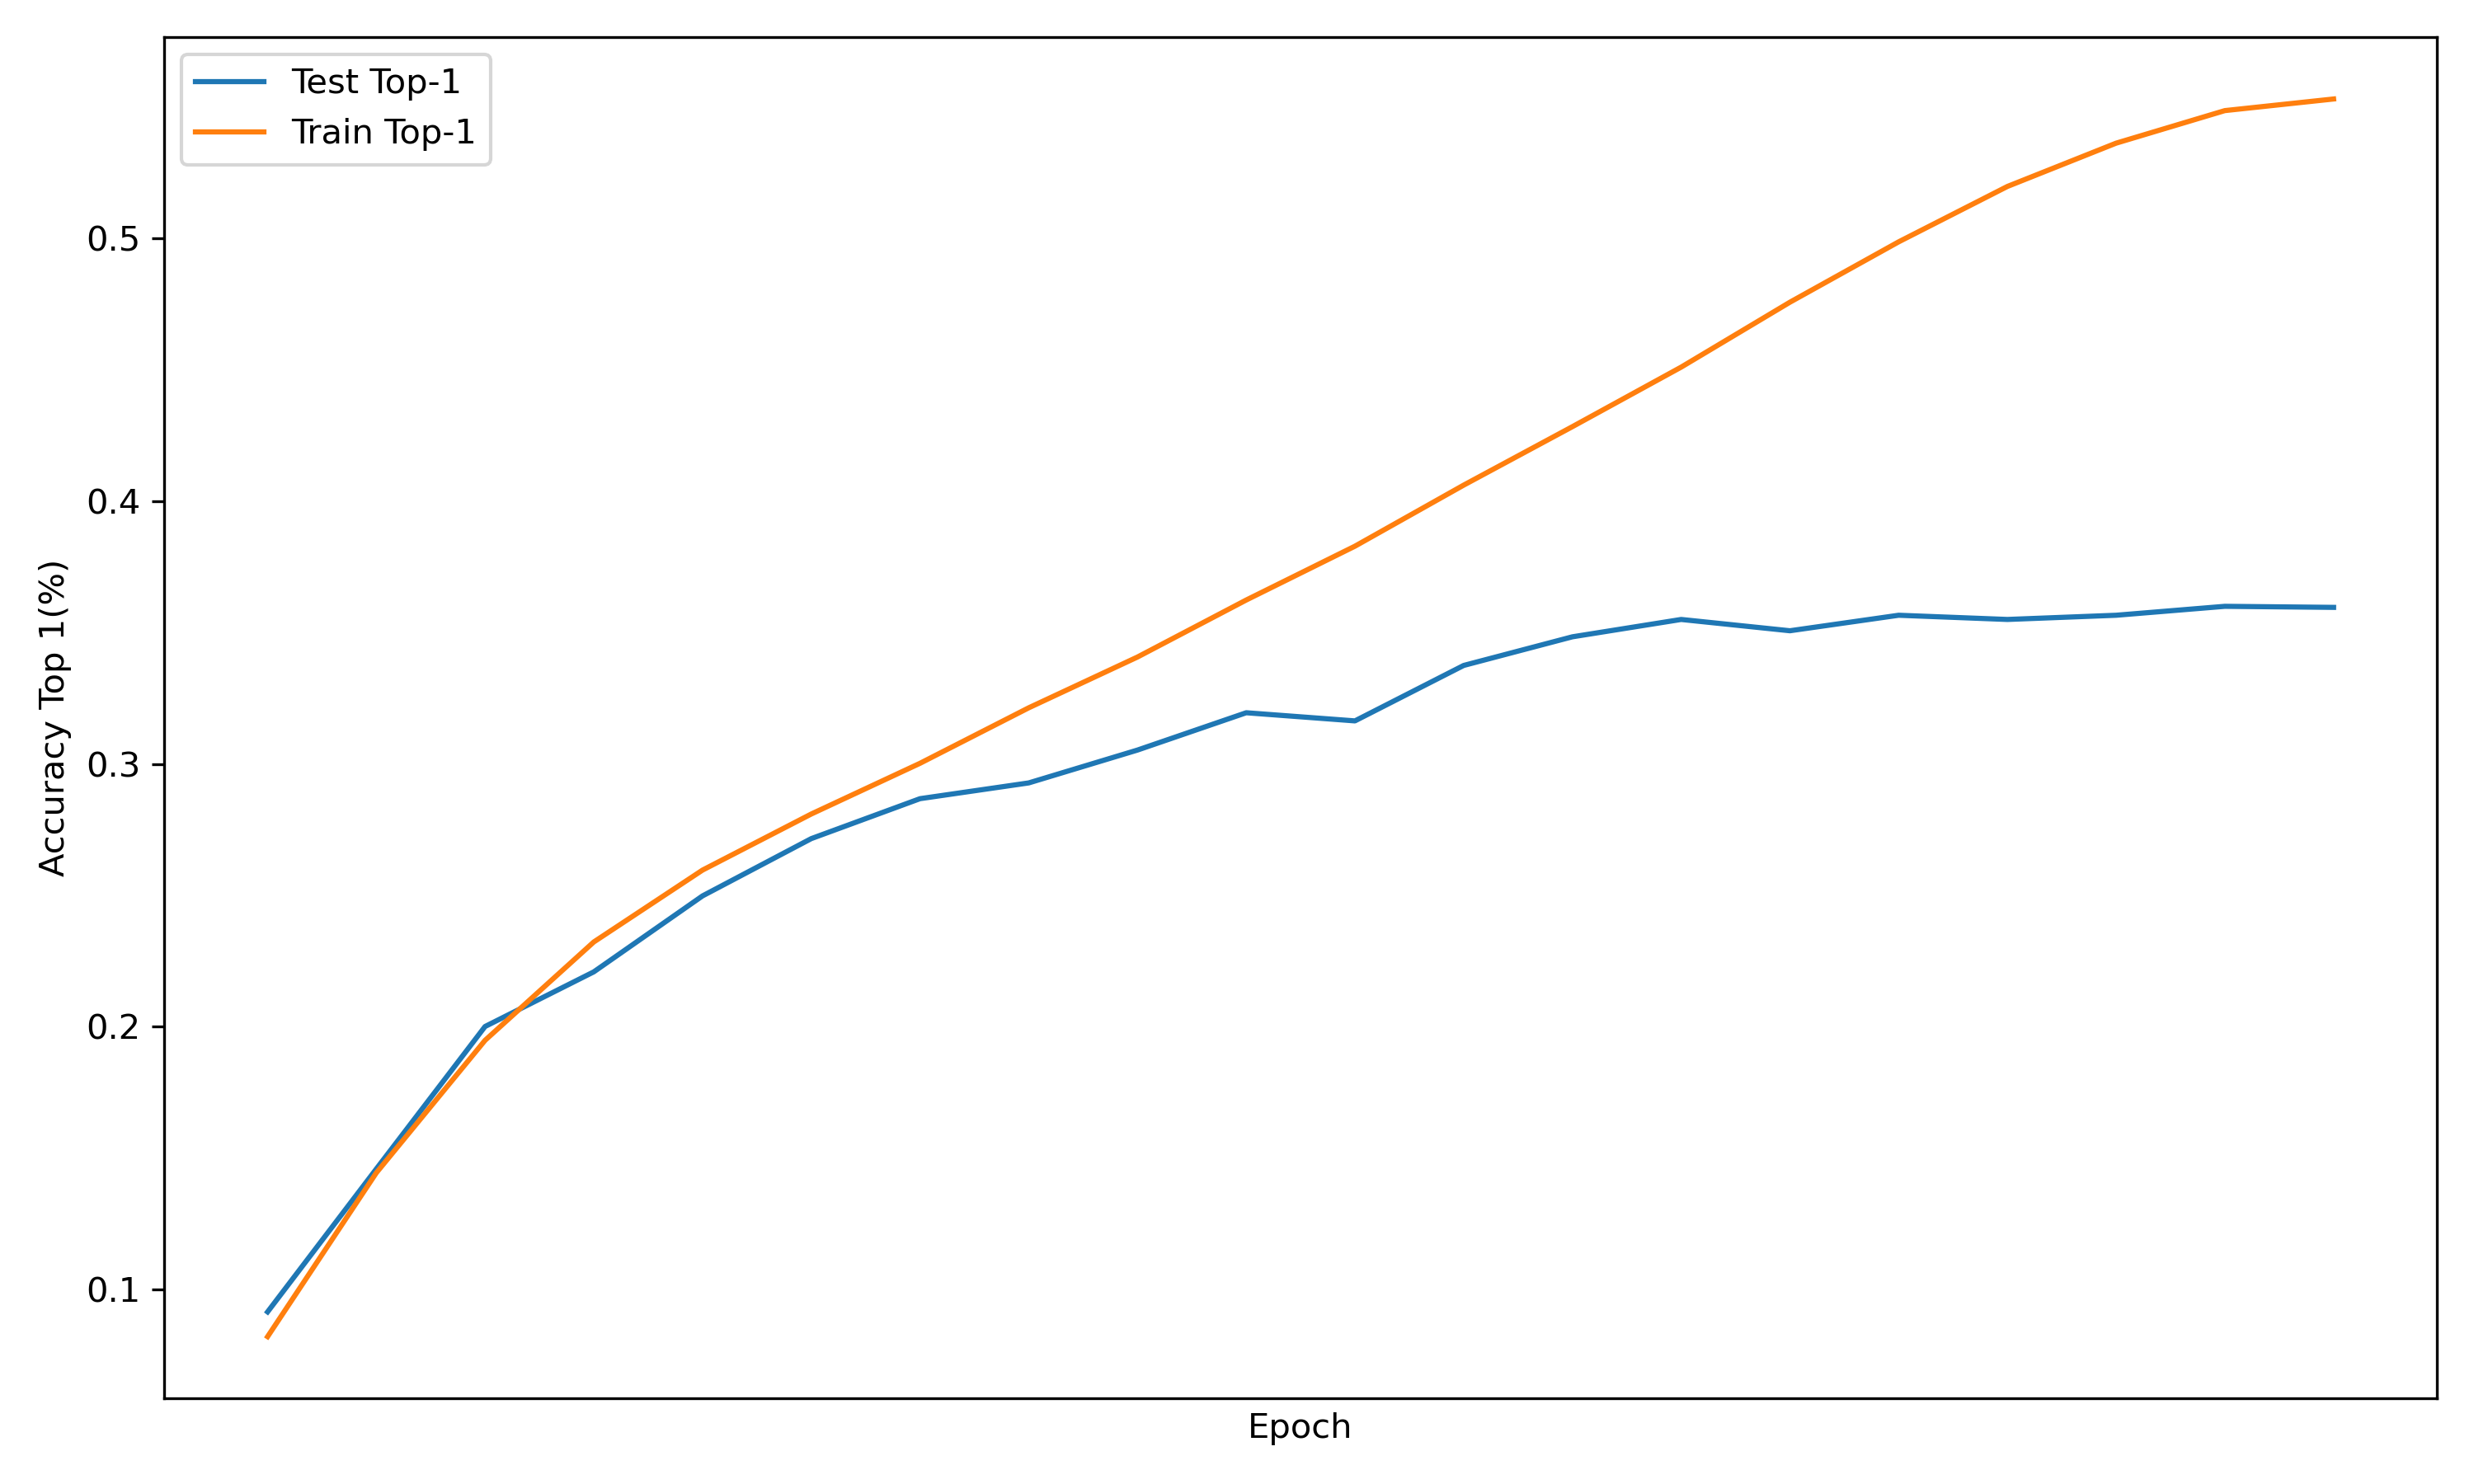
\includegraphics[width=0.85\textwidth]{transformer_images/results/tiny_image_net_tensorized.png}
	\caption{روند دقت \lr{Top-1} مدل تانسوری با بهینه‌ساز \lr{AdamW} بر روی \lr{Tiny ImageNet}.}
	\label{fig:tiny_tensor_adamw}
\end{figure}

\subsection{تحلیل و بحث}

بر اساس جدول \ref{tab:tinyimagenet_summary} و نمودارهای ارائه شده، نکات زیر قابل توجه است:
\begin{itemize}
	\item \textbf{بیش‌برازش در مدل اصلی:} مدل \lr{Tiny Swin} با وجود تعداد بالای پارامترها (\lr{27,528,690}) توانسته دقت آزمون \lr{Top-1} معقولی (\lr{64.14\%}) بدست آورد، اما اختلاف زیاد بین دقت آموزش (\lr{42.26\%}) و آزمون نشان‌دهنده ناتوانی در یادگیری کامل ویژگی‌ها و احتمال وجود محدودیت در داده یا تنظیمات بهینه‌سازی است.
	\item \textbf{بیش‌برازش شدید در مدل تانسوری با Adam:} مدل تانسوری با بهینه‌ساز \lr{Adam} دقت آموزش بسیار بالایی (\lr{83.89\%} Top-1) دارد، اما دقت آزمون آن به شدت افت کرده (\lr{30.85\%} Top-1)، که نشانه‌ی آشکار \lr{overfitting} است.
	\item \textbf{بهبود تعادل با AdamW:} تغییر بهینه‌ساز به \lr{AdamW} باعث شده شکاف آموزش–آزمون کاهش یابد و عملکرد آزمون (\lr{35.90\%} Top-1) نسبت به حالت \lr{Adam} بهبود پیدا کند، هرچند همچنان فاصله‌ی زیادی تا مدل اصلی وجود دارد.
	\item \textbf{تأثیر پیچیدگی داده:} نتایج نشان می‌دهد که کاهش شدید پارامترها در دیتاست‌های پیچیده‌تر مانند \lr{Tiny ImageNet} ممکن است منجر به کاهش توان مدل در تعمیم‌پذیری شود، مگر این که تکنیک‌های منظم‌سازی و بهینه‌سازی به درستی انتخاب شوند.
\end{itemize}

\paragraph{جمع‌بندی.} برخلاف نتایج موفقیت‌آمیز بر روی \lr{CIFAR-10} و \lr{MNIST}، در دیتاست \lr{Tiny ImageNet} کاهش پارامترها و استفاده از فشرده‌سازی تانسوری، به دلیل پیچیدگی بالای داده و محدودیت ظرفیت مدل، منجر به افت عملکرد آزمون شده است. با این حال، استفاده از بهینه‌ساز مناسب مانند \lr{AdamW} توانسته تا حدی این شکاف را کاهش دهد.










\include{chapter5}
\include{references}
\small
\csname@twosidefalse\endcsname
\pagestyle{fancy}
\fancyhf{} 
\fancyhead[RE]{\rightmark}
\fancyhead[LO]{\leftmark}
\fancyhead[LE,RO]{\thepage}
%\setLTRbibitems
%\resetlatinfont
%\latin
%\renewcommand{\bibname}{\rl{{کتاب‌نامه}\hfill}}
%\renewcommand{\refname}{\rl{{کتاب‌نامه}\hfill}}
\setLTRbibitems
\cfoot{}
\lhead{کتاب‌نامه}
\bibliographystyle{plain}
\bibliography{reference}

}
\appendix
\chapter{جزئیات مدل‌ها و جدول پارامترها}


{\baselineskip=.75cm
%\addcontentsline{toc}{chapter}{نام‌نامه}
\thispagestyle{empty}
\chapter*{\centering{نام‌نامه}}
\markboth{نام‌نامه}{نام‌نامه}
%
%ا          
%
\noindent
%\persiangloss{}{}
\persiangloss{آلبرت}{Albert}
\persiangloss{آئرتس}{Aerts}
\persiangloss{ادی}{Eddy}
\persiangloss{اگرستی}{Agresti}
\persiangloss{اُلکین}{Olkin}
\persiangloss{استفانسکی}{Stefanski}
\persiangloss{اسكندری}{Eskandari}
\persiangloss{اشپیگل‌هالتر}{Spiegelhalter}
\persiangloss{اُكانا-ریولا}{Oca\~na-Riola}
\persiangloss{اندرسون}{Anderson}
\persiangloss{اُهارا هاینز }{O'Hara Hines}
%\persiangloss{}{}
%
%     ب   
%\persiangloss{}{}
\persiangloss{بارتولومف}{Bartholomew}
\persiangloss{بریتنر}{Breitner}
\persiangloss{بهرامی سامانی}{Bahrami Samani}
%
%
%         پ%
%\persiangloss{}{}
\persiangloss{پرز}{P\'erez-Oc\'on}
\persiangloss{پرنتیس}{Prentice}
\persiangloss{پلاکت}{Plackett}
%
%            ت
%\persiangloss{}{}
\persiangloss{تات}{Tate}
\persiangloss{تاتز}{Tutz}
\persiangloss{تی‌سای}{Tsay}
%
%            ث
%
%            ج 
%
%\persiangloss{}{}
\persiangloss{جانسون}{Johnson}
\persiangloss{جفریز}{Jeffreys}
%
%چ             
%
%\persiangloss{}{}
\persiangloss{چان}{Chan}
\persiangloss{چاو}{Chau}
\persiangloss{چتفیلد}{Chatfield}
%
%‌ ح           
% خ             
%
% د               
 %
%\persiangloss{}{}
\persiangloss{دمپستر}{Dempster}
\persiangloss{دی}{Dey}
\persiangloss{دیگل}{Diggle}
\persiangloss{دیل}{Dale}
 %
% ذ             
%
%  ر 
 %
\persiangloss{رابنستین}{Rubinstein}   
\persiangloss{رابین}{Rubin}
\persiangloss{رضایی}{Rezaee}
\persiangloss{رضایی قهرودی}{Rezaei Ghahroodi}
\persiangloss{رفتری}{Raftery}
\persiangloss{ریان}{Ryan}
\persiangloss{ریدات}{Ridout}
%\persiangloss{}{}
% 
%  ز              %
%\persiangloss{}{}
\persiangloss{زگر }{Zeger}
%
% ‌ ژ             
%
%  س            ‌%
%\persiangloss{}{}
\persiangloss{سامر}{Sommer}
\persiangloss{سانگ}{Sung}
%
%   ش      %
%\persiangloss{}{}
\persiangloss{شفر}{Schafer}
\persiangloss{شلاتچر}{Schluchter}
\persiangloss{شیه}{Shih}
%        ص       
%      ض 
%   ط           
%     ظ           
%\persiangloss{}{}
%     ع         
%     غ           
%     ف          %
%\persiangloss{}{}
\persiangloss{فایندلی}{Findlay}
\persiangloss{فرانکوم}{Francom}
\persiangloss{فلر}{Feller}
\persiangloss{فهرمير}{Fahrmeir}
\persiangloss{فیتز موریس}{Fitzmaurice}
%     ق  
% ک           %
%\persiangloss{}{}
\persiangloss{کاتالانو}{Catalano}
\persiangloss{کارول}{Carroll}
\persiangloss{کاس}{Kass}
\persiangloss{کافمن}{Kaufmann}
\persiangloss{کاکس}{Cox}
\persiangloss{کاکیش}{Qaqish}
\persiangloss{كالبفلیش}{Kalbfleisch}
\persiangloss{کروسکال}{Kruskal}
\persiangloss{كنوارد}{Kenward}
\persiangloss{کورن}{Korn}
\persiangloss{کولینز}{Collins}
% گ          %
%\persiangloss{}{}
\persiangloss{گابریل}{Gabriel}
\persiangloss{گلفند}{Gelfand}
\persiangloss{گنجعلی}{Ganjali}
\persiangloss{گود}{Good}
\persiangloss{گودمن}{Goodman}
\persiangloss{گیسر}{Geisser}
%
%
 %
%
%   ل         %
%\persiangloss{}{}
\persiangloss{لان}{Lunn}
\persiangloss{لایرد}{Laird}
\persiangloss{لاولس}{Lawless}
\persiangloss{لسافره}{Lesaffre}
\persiangloss{لیانگ}{Liang}
\persiangloss{لیپ‌شیتز}{Lipsitz}
\persiangloss{لیتل}{Little}
\persiangloss{لیندلی}{Lindley}
%
%     م        %
%\persiangloss{}{}
\persiangloss{مادیگان}{Madigan}
\persiangloss{مشكانی}{Meshkani}
\persiangloss{موری}{Murray}
\persiangloss{مولنبرگز}{Molenberghs}  
\persiangloss{موئنز}{Muenz}
\persiangloss{مه‌کولا}{McCullagh}
\persiangloss{مه‌کوله}{McCulloch}
\persiangloss{مید}{Mead}
%       ن     %
%\persiangloss{}{}
\persiangloss{ناگل‌كرك}{Nagelkerke}
\persiangloss{نلدر}{Nelder}
\persiangloss{نوریان}{Noorian}
\persiangloss{نیوتن}{Newton}
\persiangloss{نیوهاز}{Neuhaus}
%
%
%          و %
%\persiangloss{}{}
\persiangloss{ودربرن}{Wedderburn}
\persiangloss{وربک}{ٰVerbeke}
\persiangloss{ورموت}{Wermuth}
\persiangloss{وُنگ}{Wong}
\persiangloss{وو}{Wu}
\persiangloss{ویت‌مور}{Whittemore}
\persiangloss{وِیر}{Ware}
%               ه        %
%\persiangloss{}{}
%\persiangloss{هارویل}{Harville}
\persiangloss{هکمن}{Heckman}
%\persiangloss{هندرسون}{Henderson}
\persiangloss{هیتچکاک}{Hitchcock}
\persiangloss{هاینز}{Hines}
%
%            ی 
%\persiangloss{}{}
\persiangloss{یانگ}{Yang}
%  
%
%\addcontentsline{toc}{chapter}{واژه‌نامه فارسی به انگلیسی}
%\thispagestyle{empty}
\chapter*{\centering{واژه‌نامه فارسی به انگلیسی}}
\markboth{واژه‌نامه فارسی به انگلیسی}{واژه‌نامه فارسی به انگلیسی}

\noindent
%\englishgloss{}{}
\englishgloss{Cross-Over Trials}{آزمایه‌های متقاطع}
\englishgloss{Peabody Individual Achievement Test (PIAT)}{آزمون انفرادی  پيشرفت پی‌بادی}
\englishgloss{Equilibrium Probability}{احتمال  تعادل}
\englishgloss{Nelder and Mead Simplex Algorithm}{الگوریتم سادکی نلدر و مید}
\englishgloss{Insomnia}{بی‌خوابی}
\englishgloss{Parsimonious Parametrization}{پارامتریدن ممسك}
\englishgloss{Link Function}{تابع ربط}
\englishgloss{Exchangeable}{تبادل‌پذیر}
\englishgloss{Mastitis Data}{داده‌های آماس غده‌ها}
\englishgloss{Xerophthalmia}{رمد چشم}
\englishgloss{Absorbing Markov chain}{زنجیر مارکوف جاذب}
\englishgloss{Non-homogeneous Markov Chain}{زنجیر مارکوف ناهمگن}
\englishgloss{Identifiability}{شناسایی‌پذیری}
\englishgloss{Innovation}{عامل ابداع}
\englishgloss{Conditional Predictive Ordinate (CPO)}{عرض پیشگوی شرطی}
\englishgloss{Irreversible Process}{فرایند برگشت‌ناپذیر}
\englishgloss{Serially Correlated Process}{فرایند همبسته‌ی پیاپی}
\englishgloss{Quadrature Formula}{فرمول تربیعی}
\englishgloss{Fluvoxamine}{فلووکسامین}
\englishgloss{Discriminant Analysis Applications}{كاربردهای تحلیل  تشخیصی}
\englishgloss{Latent Variable}{متغیر پنهان}
\englishgloss{Bayesian Generalized Additive Mixed Model}{مدل آمیخته جمعی تعمیم‌یافته بیزی}
\englishgloss{Random-Coefficient Pattern-Mixture Models}{مدل‌های الگو  آمیخته‌ی ضرایب تصادفی}
\englishgloss{Random-Coefficient Selection Models}{مدل‌های گزینش ضرایب تصادفی}
\englishgloss{Likelihood Based Mixture Parameter Model}{مدل  پارامتر آمیخته  مبتنی بر درستنمایی}
\englishgloss{Subject-Specific Model}{مدل خاص آزمودنی}
\englishgloss{General Location Model}{مدل مکانی عام}
\englishgloss{Population-Averaged Model}{مدل  میانگین-جامعه}
\englishgloss{Generalized Heckman Model}{مدل هكمن تعمیم‌یافته}
\englishgloss{Indonesian Children's Health Study}{مطالعه سلامت کودکان اندونزیایی}
\englishgloss{Score Equations}{معادله‌های امتیاز}
\englishgloss{Generalized Estimating Equations}{معادله‌های  برآوردساز تعمیم‌یافته}
\englishgloss{Deviance Information Criterion (DIC)}{ملاک اطلاع انحرافه}
\englishgloss{Cut-Point}{نقطه‌ی برش}
\englishgloss{Change Point}{نقطه‌ی تغییر}
\englishgloss{Isotonic}{همنوا}
\englishgloss{m-Dependence}{$m$-وابستگی}
%
%\addcontentsline{toc}{chapter}{واژه‌نامه  انگلیسی به  فارسی}
\thispagestyle{empty}
\chapter*{\centering{واژه‌نامه  انگلیسی به  فارسی}}
\markboth{واژه‌نامه  انگلیسی به  فارسی}{واژه‌نامه  انگلیسی به  فارسی}

\noindent
\persiangloss{شکنندگی}{Frailty}
\persiangloss{مدل نرخ خطرهای متناسب کاکس}{Proportional Hazards Rate Model}
\persiangloss{مطالعات خانوادگی}{Familial Studies}
\persiangloss{آزمایه‌های بالینی چندمرکزی}{Multicenter clinicla trials}
\persiangloss{استقلال بین خوشه‌ای}{Intercluster Independence}
\persiangloss{شناسایی‌پذیر}{Identifiable}
\persiangloss{داده‌های بقای فضایی}{Spatial Survival Data}
\persiangloss{استقلال بین خوشه‌ای}{Intercluster Independence}
\persiangloss{استقلال بین خوشه‌ای}{Intercluster Independence}
\persiangloss{استقلال بین خوشه‌ای}{Intercluster Independence}
\persiangloss{استقلال بین خوشه‌ای}{Intercluster Independence}
\persiangloss{استقلال بین خوشه‌ای}{Intercluster Independence}
\printindex
% در این فایل، عنوان پایان‌نامه، مشخصات خود و چکیده پایان‌نامه را به انگلیسی، وارد کنید.
% توجه داشته باشید که جدول حاوی مشخصات پایان‌نامه/رساله، به طور خودکار، رسم می‌شود.
%%%%%%%%%%%%%%%%%%%%%%%%%%%%%%%%%%%%
\baselineskip=.6cm
\begin{latin}
\latintitle{Analysis of brain data using graph neural networks}
\latinuniversity{Tarbiat Modares University}
\latinfaculty{Faculty of Mathematical Sciences}
\latindegree{Master in Computer Science}
%group:
\latinsubject{Department of Mathamatiics}
\latinfield{}
\latintitle{Vision Trnasformer}
\firstlatinsupervisor{Dr. Mansoor Rezghi }
%\secondlatinsupervisor{Second Supervisor}
%\firstlatinadvisor{First Advisor}
%\secondlatinadvisor{Second Advisor}
\latinname{Seyed Mohammad}
\latinsurname{Badzohreh}
\latinthesisdate{2024}
\latinkeywords{ }

\newpage
\thispagestyle{empty}
\baselineskip=.750cm
\en-abstract{%\noindent
Some data that present the time ...
}


%\markboth{\lr{Abstract}}{\lr{Abstract}}
\noindent
\begin{large}
\begin{center}
Abstract
\end{center}
\end{large}
%

In recent years, vision transformers have emerged as one of the core architectures in deep learning models for image processing. However, conventional designs of these transformers often rely on fully connected layers that require flattening high-order input tensors into vectors. This process not only leads to a significant increase in the number of parameters but also results in the loss of spatial structures and inter-dimensional relationships within the data. In this study, we propose a tensor-based framework for the design of a window-based vision transformer that leverages Tensor Compression Layers (TCL) and Tensor Regression Layers (TRL) to effectively model multilinear mappings across data dimensions. By preserving the multidimensional structure of images, the proposed method achieves a substantial reduction in the number of parameters while maintaining structural information and improving the interpretability of the model. Experimental results on standard benchmark datasets demonstrate that incorporating tensorized structures not only reduces computational complexity but also enhances classification accuracy.
\\
\newline
{{\bf Key Words:}} Vision Transformer, Tensor Decomposition, Tensor Compression Layer (TCL), Tensor Regression Layer (TRL), Multilinear Mapping, Image Classification, Deep Learning.%}
\newpage
\latinvtitle
%
%\latintitle{Analysis of brain data using graph neural networks}
%\latinuniversity{Tarbiat Modares University}
%\latinfaculty{Faculty of Mathematical Sciences}
%\latindegree{Master in Computer Science}
%%group:
%\latinsubject{Department of Mathamatiics}
%\latinfield{}
%\latintitle{Analysis of brain data using graph neural networks}
%\firstlatinsupervisor{Mansour Rezghi Ahagh}
%%\secondlatinsupervisor{Second Supervisor}
%%\firstlatinadvisor{First Advisor}
%%\secondlatinadvisor{Second Advisor}
%\latinname{Mitra}
%\latinsurname{Nemati Andavari}
%\latinthesisdate{2024}
%\latinkeywords{ }
\end{latin}
}
\label{LastPage}
\end{document}